\documentclass[12pt]{../packages/thesis}  %12pt is larger than 11pt

\usepackage{titlesec}
   \titleformat{\chapter}
      {\normalfont\large}{Chapter \thechapter:}{1em}{}

\usepackage[pdftex]{graphicx}
\usepackage{mathrsfs,amsmath,amssymb, amsfonts}

\numberwithin{equation}{chapter}
\setcounter{secnumdepth}{4}
\titleformat{\paragraph}
{\normalfont\normalsize\bfseries}{\theparagraph}{1em}{}
\titlespacing*{\paragraph}
{0pt}{3.25ex plus 1ex minus .2ex}{1.5ex plus .2ex}
\usepackage{chngcntr}
\usepackage{float}
\counterwithin{table}{chapter}
\counterwithin{figure}{chapter}
\usepackage{cite}
\usepackage{lscape}
\usepackage{indentfirst}
\usepackage{latexsym}
\usepackage{multirow}
\usepackage{tabls}
\usepackage{wrapfig}
\usepackage{../packages/slashbox}
\usepackage{longtable}
\usepackage{supertabular}
\usepackage{subfigure}
\usepackage{standalone}


\newcommand{\tbsp}{\rule{0pt}{18pt}} %used to get a vertical distance after \hline
\renewcommand{\baselinestretch}{2}
\setlength{\textwidth}{5.9in}
\setlength{\textheight}{9in}
\setlength{\topmargin}{-.50in}
%\setlength{\topmargin}{0in}    %use this setting if the printer makes the the top margin 1/2 inch instead of 1 inch
\setlength{\oddsidemargin}{.55in}
\setlength{\parindent}{.4in}
\pagestyle{empty}

\begin{document}


%\input{Abstract} %(must be first, required, non-numbered)
\titlepage
\thispagestyle{fancy}
\begin{center}
\vspace*{50pt}
{\huge \bfseries Multistatic RF Sensor Networks in Maritime Environments\\}
\vspace{75 pt}

\Large Ben Frazier \\
\Large Sheldon Bish \\
\large IRST and Sensors Group (FPS/KVU)\\
\vspace{25pt}
\large \today \\

\begin{figure*}[!b]
\begin{center}

\includegraphics[width=0.75\textwidth]{../media/FP_Blue.png}
\end{center}
\end{figure*}

\end{center} %(must follow Abstract, required, non-numbered)
\newpage
%%Copyright

\thispagestyle{empty}
\hbox{\ }

\vfill
\renewcommand{\baselinestretch}{1}
\small\normalsize

\vspace{-.65in}

\begin{center}
\large{\copyright \hbox{ }Copyright by\\
Benjamin W. Frazier %Type your name as it appears in University records
\\
2017}
\end{center}
\vfill %(highly recommended, non-numbered)

%Pages from this point start at lower-case Roman number ii)
\pagestyle{plain}
\pagenumbering{roman}
\setcounter{page}{2}

%%Preface

\renewcommand{\baselinestretch}{2}
\small\normalsize
\hbox{\ }
 
\vspace{-.65in}

\begin{center}
\large{Preface} 
\end{center} 


If needed.
  %(if present, start at lower-case Roman number ii)
%%Foreword

\renewcommand{\baselinestretch}{2}
\small\normalsize
\hbox{\ }
 
\vspace{-.65in}

\begin{center}
\large{Foreword} 
\end{center} 

If needed.
 %(if present, lower-case Roman)
%%Dedication

\renewcommand{\baselinestretch}{2}
\small\normalsize
\hbox{\ }
 
\vspace{-.65in}

\begin{center}
\large{Dedication}
\end{center} 

If needed.
 %(if present, lower-case Roman)
%%Acknowledgments

\renewcommand{\baselinestretch}{2}
\small\normalsize
\hbox{\ }
 
\vspace{-.65in}

\begin{center}
\large{Acknowledgments} 
\end{center} 

\vspace{1ex}

I owe my gratitude to all the people who have made this thesis possible and because of whom my graduate experience has been one that I will cherish forever.

First and foremost I'd like to thank my advisor, Professor Rajarshi Roy for giving me an invaluable opportunity to work on challenging and extremely interesting projects over the past four years. He has always made himself available for help and advice and there has never been an occasion when I've knocked on his door and he hasn't given me time. It has been a pleasure to work with and learn from such an extraordinary individual.

I would also like to thank my co-advisor, Dr. Parvez Guzdar. Without his extraordinary theoretical ideas and computational expertise, this thesis would have been a distant dream. Thanks are due to Professor Robert Gammon, Professor Edward Ott and Professor Thomas Antonsen for agreeing to serve on my thesis committee and for sparing their invaluable time reviewing the manuscript.

My colleagues at the nonlinear optics laboratory have enriched my graduate life in many ways and deserve a special mention. David DeShazer helped me start-off by rewriting the basic simulation code in a user-friendly format. Christian Silva provided help by setting up the GRENOUILLE apparatus and performing some of the simulations. My interaction with  Rohit Tripathi, Ryan McAllister, Vasily Dronov, Min-Young Kim, Elizabeth Rogers, William Ray, Jordi Garcia Ojalvo, Riccardo Meucci, Atsushi Uchida, and Fabian Rogister has been very fruitful. I'd also like to thank Wing-Shun Lam and Benjamin Zeff for providing the LaTex style files for writing this thesis.

I would also like to acknowledge help and support from some of the staff members. Donald Martin's technical help is highly appreciated, as is the computer hardware support from Edward Condon, LaTex and software help from Dorothea Brosius and purchasing help from Nancy Boone.

I owe my deepest thanks to my family - my mother and father who have always stood by me and guided me through my career, and have pulled me through against impossible odds at times. Words cannot express the gratitude I owe them. I would also like to thank Dr. Mohan Advani, Dr. Vasudeo Paralikar and Dr. Vinod Chaugule who are like family members to me.

My housemates at my place of residence have been a crucial factor in my finishing smoothly. I'd like to express my gratitude to Sivasankar Pandeti, Jayakumar Patil, Amit Trehan and Punyaslok Purakayastha for their friendship and support.

I would like to acknowledge financial support from the Office of Naval Research (ONR), Physics, for all the projects discussed herein.

It is impossible to remember all, and I apologize to those I've inadvertently left out.

Lastly, thank you all and thank God!
 %(if present, lower-case Roman)

\renewcommand{\baselinestretch}{1}
\small\normalsize
\tableofcontents %(required, lower-case Roman)
\newpage
\listoffigures %(if present, lower-case Roman)
\newpage
%List of Abbreviations
\addcontentsline{toc}{chapter}{List of Abbreviations}
%List of Abbreviations


\renewcommand{\baselinestretch}{1}
\small\normalsize
\hbox{\ }

\vspace{-4em}

\begin{center}
\large{List of Abbreviations}
\end{center} 

\vspace{3pt}

\begin{supertabular}{ll}
CPI & Coherent Processing Interval \\
FFT & Fast Fourier Transform \\
JHU/APL & Johns Hopkins University Applied Physics Laboratory \\
JONSWAP & Joint North Sea Wave Project\\
OSG & Ocean Surface Generator \\
PDF & Probability Distribution Function \\
PM & Pierson-Moskowitz \\
RCS & RADAR Cross Section \\
RF & Radio Frequency \\
SCR & Signal to Clutter Ratio \\
SNR & Signal to Noise Ratio\\
TEMPER & Tropospheric Electromagnetic Parabolic Equation Routine \\
WGS & World Geodetic System \\
WMO & World Meterological Organization \\
\end{supertabular}

\newpage
%List of Symbols
\addcontentsline{toc}{chapter}{List of Symbols}
%List of Symbols
\renewcommand{\baselinestretch}{1}
\small\normalsize
\hbox{\ }

\begin{center}
\large{List of Symbols}
\end{center} 

\vspace{3pt}

\begin{supertabular}{ll}
%lowercase variables
$c$ & Speed of light \\
$f$ & Temporal frequency \\
$f_x$ & Spatial frequency along $x$ \\
$f_y$ & Spatial frequency along $y$ \\
$g$ & Coefficient of gravity \\
$h_1$ & Transmitter altitude\\
$h_2$ & Target altitude \\
$j$ & Complex numer, $\sqrt{-1}$ \\
$k$ & Spatial frequency (wave number) \\
$k_o$ & Wave number \\
$k_B$ & Boltzmann constant \\
$k_p$ & Wave number of the spectral peak \\
$n$ & Index of refraction \\
$\hat{n}$ & Surface normal (pointing outward) \\
$\mathbf{r}$ & Position vector to observer \\
$\mathbf{r}'$ & Position vector to source \\
$r_e$ & Radius of the earth \\
$r_e'$ & 4/3 effective radius of the earth \\
$v$ & Ocean wave phase speed \\
$x_m$ & Primary reflection point \\
\\
%uppercase variables
$\mathbf{A}$ & Vector potential \\
$B$ & Receiver bandwidth \\
$\mathcal{C}$ & Complex contour \\
$\mathcal{F}\{\}$ & Fourier transform \\
$\mathcal{F}^{-1}\{\}$ & Inverse Fourier transform \\
$F_n$ & Receiver noise bandwidth \\
$F_p$ & Propagation factor \\
$G$ & Green's function \\
$G_o$ & Free space Green's function \\
$G_r$ & Receiver antenna gain \\
$G_t$ & Transmitter antenna gain \\
$H(t-t_0)$ & Heaviside step function \\
$H_0^{(1)}$ & Hankel function of the first kind \\
$H_0^{(2)}$ & Hankel function of the second kind \\
$H_{1/3}$ & Significant wave height \\
$I_0$ & Modified Bessel function of the first kind \\
$J_0$ & Bessel function of the first kind \\
$L$ & Spatial domain length \\
$L_r$ & Reflected ray path length \\
$L_s$ & Random component of reflected ray path \\
$L_{so}$ & Shortest orbit paths of reflected ray \\
$L_0$ & Deterministic component of reflected ray path \\
$L_0''$ & Second derivative of $L_0$ evaluated at $x_m$ for Taylor expansion\\
$M$ & Modified index of refraction \\
$N_0$ & Bessel function of the second kind \\
$N$ & Number of points \\
$P_d$ & Probability of detection \\
$P_n$ & Noise power\\
$P_r$ & Received power \\
$P_t$ & Transmitted power \\
$R$ & Slant range \\
$R_h$ & Slant range to horizon \\
$R_1$ & Slant range along 1st path \\
$R_2$ & Slant range along 2nd path \\
$S$ & 1-D Power spectral density \\
$T$ & Temperature \\
$U_{10}$ & Wind speed at $10$ m altitude \\
$U_{19}$ & Wind speed at $19$ m altitude \\
$V$ & Frequency domain representation of sea surface\\
\\
%greek variables
$\alpha$ & Depression angle \\
$\beta$ & Bistatic angle \\
$\delta\left(\mathbf{r}-\mathbf{r}' \right)$ & Dirac delta function \\
$\Gamma$ & Smooth sea surface (Fresnel) reflection coefficient \\
$\Gamma_t$ & Total reflection coefficient \\
$\Gamma_1$ & Reflection coefficient at primary reflection point\\
$\rho$ & Rough sea surface reflection coefficient \\
$\lambda$ & Wavelength \\
$\sigma$ & Target RCS\\
$\sigma_B$ & Target Bistatic RCS \\
$\sigma_h$ & RMS wave height \\
$\sigma_s$ & Conductivity of sea water \\
$\sigma_0$ & Clutter backscatter coefficient \\
$\Delta k$ & Spectral domain sampling step \\
$\Delta x$ & Spatial domain sampling step \\
$\epsilon_r$ & Relative permittivity \\
$\Omega$ & Inverse age parameter \\
$\theta$ & One way antenna beam width \\
$\theta_2$ & Two way antenna beam width \\
$\chi$ & Grazing angle \\
$\Psi $ & 2-D Power spectral density \\
\end{supertabular}
\newpage

\setlength{\parskip}{0em}
\renewcommand{\baselinestretch}{2}
\small\normalsize

%Pages from this point start at Arabic numeral 1
%Pages from this point start at Arabic numeral 1
\setcounter{page}{1}
\pagenumbering{arabic}

\renewcommand{\thechapter}{1}
\renewcommand{\baselinestretch}{2} \small\normalsize
\chapter{Introduction and Background}
Analysis of RADAR systems in maritime environments is complicated by the fact that the ocean does not generally provide a smooth or uniform surface to work with. Altitude variations change the aspect angle for multipath bounces, induce wave blockage, and add clutter and spikes to the echo return \cite{skolnik_handbook}, \cite{blake_radar}, \cite{nathanson_radar}. Understanding the impact of the sea surface on propagation is critical to evaluating the performance of a RADAR system in a maritime environment.

This chapter discusses the concept of a multistatic RF sensor network in a maritime environment and then covers some RADAR basics. The background described here defines the one and two way antenna beam widths, develops the RADAR range equation for both monostatic and bistatic configurations, and introduces the theory behind probability of detection.

\section{Multistatic RF Sensor Network Concept}
When we look at cases where the transmitter and receiver are not colocated, we have a bistatic system and analyzing performance becomes even more difficult \cite{willis_bistatic}. With additional receivers or transmitters, the configuration is termed multistatic as it has multiple bistatic elements. Of particular concern for this document is the case with a single transmitter and multiple receivers.

An example multistatic RF sensor network in a maritime environment is shown in Figure \ref{ms_fig:1}. In this concept, a single transmitter illuminates a target and the echo signal is captured by a pair of receivers. The received signal will fluctuate due to multipath reflections from the surface, path variations, and relative motion of the target. In order to determine the probability of the target being detected by either receiver, we need to understand the statistics of the received signals.

\begin{figure}[H]
  \begin{center}
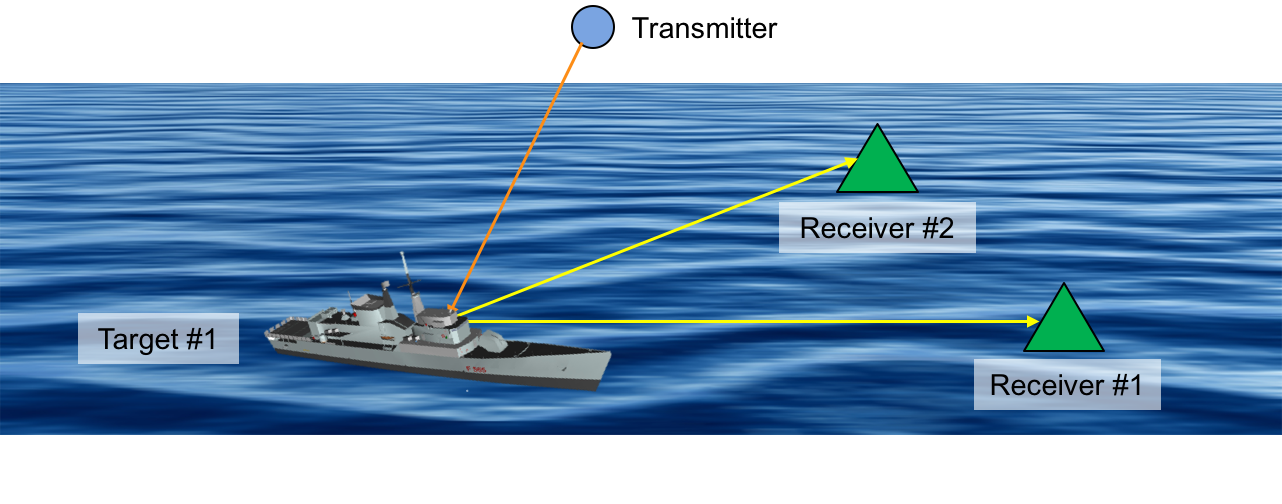
\includegraphics[width=5in]{../media/multistatic/ms_rf_concept.png}
  \end{center}
  \renewcommand{\baselinestretch}{1} \small\normalsize
  \begin{quote}
    \caption[Multistatic RF Sensor Networks Concept]{Multistatic RF Sensor Networks Concept\label{ms_fig:1}}
  \end{quote}
\end{figure}
\renewcommand{\baselinestretch}{2} \small\normalsize

\section{Beam Width}
The beam width of an antenna is defined as the angle between the half power points in the antenna pattern.

\subsection{One Way}
The one way antenna beam width, $\theta$, is simply the beam width of the forward propagating beam.

\subsection{Two Way}
The two way antenna beam width, $\theta_2$, is the beam width of the return beam that propagates in both directions. For the monostatic case, we can compute this as the one way beam width of the square of the antenna pattern. In most cases, $\theta_2 \approx \frac{1}{\sqrt{2}}\theta$.

\section{RADAR Range Equation} 
The RADAR range equation provides a deterministic method to calculate received signal levels and is the workhorse for analyzing RADAR system performance. Thi equation is the first step towards building a statistical model, as it captures the underlying physics.

\subsection{Monostatic Case}
The traditional monostatic RADAR range equation is shown in Equation \ref{intro_eq:1} and is generated by assuming spherically propagating waves and taking the product of four components: the power received at the target, the power reflected by the target, the power received back at the transmitter, and the effective area of the transmitter\cite{skolnik_handbook}.
  \begin{equation}
  \label{intro_eq:1}
 P_r = \left(\frac{P_tG_t}{4\pi R^2}\right) \left(\sigma \right)\left(\frac{1}{4\pi R^2}\right)\left( \frac{G_t\lambda^2}{4\pi} \right) = \frac{P_tG_t^2\sigma\lambda^2}{\left(4\pi\right)^3R^4}
  \end{equation}
The projected power is spread out over a sphere of radius equal to the slant range, $R$, which gives the factor of $\left( 4\pi R^2 \right)^{-1}$. The total projected power is the transmitted power, $P_t$, multiplied by the antenna gain, $G_t$. The RADAR cross section (RCS), $\sigma$, defines the amount of power intercepted and reflected. The effective area of the antenna is then $\frac{G_t\lambda^2}{4\pi}$.
  
We can divide Equation \ref{intro_eq:1} by the noise power to represent the RADAR equation in terms of signal to noise ratio (SNR) as shown in Equation \ref{intro_eq:2} \cite{skolnik_handbook}.
\begin{equation}
    \label{intro_eq:2}
\text{SNR} = \frac{P_r}{P_n} = \frac{P_tG_t^2\sigma\lambda^2}{\left(4\pi\right)^3 R^4k_BTBF_n}
\end{equation}
In this equation, $k_B$ is the Boltzmann constant, $B$ is the receiver bandwidth, $T$ is the receiver temperature and $F_n$ is the receiver noise figure. Nominally, $B$ is taken to be the inverse of the pulse width to accomodate matched filter processing and $T$ is taken to be $300$ K.

\subsection{Bistatic Case}
In the bistatic case, we need to consider each path separately as the ranges, antenna gains, and RCS are all likely different. The standard bistatic RADAR range equation is shown in Equation \ref{intro_eq:3}.
  \begin{equation}
  \label{intro_eq:3}
 P_r = \frac{P_tG_tG_r\sigma_B\lambda^2}{\left(4\pi\right)^3R_1^2R_2^2}
  \end{equation}
In this equation, $G_t$ is the antenna gain for the transmitter, $G_r$ is the antenna gain for the receiver, $\sigma_B$ is the bistatic RCS, $R_1$ is the slant range along the first path, and $R_2$ is the slant range along the second path.

The bistatic RADAR range equation in terms of SNR is shown in Equation \ref{intro_eq:4}.
\begin{equation}
    \label{intro_eq:4}
\text{SNR} = \frac{P_tG_tG_r\sigma_B\lambda^2}{\left(4\pi\right)^3 R_1^2R_2^2k_BTBF_n}
\end{equation}

\subsection{Propagation Factors}
The use of propagation factors allow us to include atmospheric effects in the RADAR range equation. These effects can include absorption from atmospheric gases and weather such as rain or snow as well as rollups for the effects of multipath reflections.

\section{Probability of Detection}

\section{Processing Gains}
\subsection{Coherent Processing}
\subsection{Noncoherent Processing}
\subsection{M of N Detection}

\renewcommand{\thechapter}{2}
\chapter{Ocean Surface Modeling}
To capture the physical behavior of electromagnetic waves reflecting off the surface of the ocean, we need to model the surface altitude variations correctly. For this, we first need to understand the power spectra of ocean waves and their dependencies. Next, we can generate random realizations of sea surfaces by discretizing the power spectrum and taking the inverse Fourier transform of a Hermitian sequence of spectrally appropriate coefficients. This will be demonstrated in both the 1-dimensional and 2-dimensional cases.

\section {Waves in the Ocean}
Ocean waves are primarily driven by wind and start when turbulence creates capillary or surface waves with small wavelengths (on the order of a few centimeters). As the wind continues to blow, it increases both the amplitude and the wavelength of the waves until they start to interact. These interactions continue to increase the wavelength and phase speed of the waves until they are traveling faster than the wind, at which point the sea is deemed fully developed. As a sea develops, energy will transfer from higher frequencies to lower frequencies which means the power spectrum will be different for a younger sea than a mature one.

Before discussing the statistical properties of ocean waves, it is useful to review some standard nomenclature. Fetch is the length over which the wind can be considered constant, and a longer fetch generally means higher waves. Significant wave height is the mean wave height of the highest third of the waves. It is represented in the literature as $H_{1/3}$ and is equal to 4 times the standard deviation of the wave height, $H_{1/3} = 4\sigma_h$. Wave height generally refers to the mean difference between successive peaks and troughs (twice the amplitude).

\section{Ocean Wave Power Spectra}  \label{os_sec:power_spectra}
Many methods have been proposed to statistically describe the behavior of ocean waves. These range from the simplest sea state representations with a very coarse binning of wind speed and sea height variations to mathematically complex multi-parameter power spectra.

\subsection {Sea State}
The modern concept of sea state is a combination of the Beaufort wind scale and the Douglas sea scale. The Beaufort wind scale was developed in the early 1800s by sir Francis Beaufort and the Douglas sea scale was developed in the 1920s by H.P Douglas, both of the Royal Navy \cite{uk_met_fact_sheet6}. The Beaufort wind scale measures force vs. wind speed in 12 bins from "Calm" to "Hurricane" and was extended in 1944 to add scales up to 17. In 1960, it was further extended to add probable wave heights. 

The Douglas sea scale on the other hand measures sea height in 9 bins from "Calm (glossy)" to "Phenomenal". The Word Meterological Organization (WMO) has adopted the Douglas sea scale as a standard \cite{wmo_code} and we can compare this to the Beaufort wind scale to add the dependency on wind speed as shown in Table \ref{os_tab:0}. There are no true standards when working with sea states, so care must be taken when comparing results between research groups.

\begin{table}[H]
  \begin{center}
      \renewcommand{\baselinestretch}{1} \small\normalsize
  \begin{quote}
    \caption[WMO Sea State vs. Wind Speed and Wave Height]{WMO Sea State vs. Wind Seed and Wave Height\label{os_tab:0}}
  \end{quote}
  \begin{tabular} {|c | c | c| c|}
    \hline
  \bf{Sea State} & \bf{Descriptio}n & \bf{Wave Height (m)} & \bf{Wind Speed (m/s)}\\ \hline
  0 & Calm (glassy) & 0 & $<$ 0.3 \\ \hline
  1 & Calm (rippled) & 0 - 0.1 & 0.3 - 1.5 \\ \hline
  2 & Smooth (wavelets) & 0.1 - 0.5 & 1.6 - 3.3 \\ \hline
  3 & Slight & 0.5 - 1.25 & 3.4 - 5.5 \\ \hline
  4 & Moderate & 1.25 - 2.5 & 5.5 - 10.7 \\ \hline
  5 & Rough & 2.5 - 4 & 10.8 - 13.8 \\ \hline
  6 & Very Rough & 4 - 6 & 13.9 - 17.1\\ \hline
  7 & High & 6 - 9 & 17.2 - 24.4\\ \hline
  8 & Very High & 9 - 14 & 24.5 - 32.6\\ \hline
  9 & Phenomenal & $\geq$ 14 & $\geq$ 32.7\\ \hline
\end{tabular}
\end{center}
\end{table}
\renewcommand{\baselinestretch}{2} \small\normalsize

\subsection{Pierson-Moskowitz Spectrum}
In 1964, the Pierson-Moskowitz (PM) spectrum given in Equation \ref{os_eq:1} was developed to describe the power spectrum of the variance of wave height in terms of the measured wind speed 19 meters above the sea surface ($U_{19}$) \cite{michel_sea_spectra}. 
 \begin{equation}
S(k) = \frac{0.0081}{k^3}e^{-0.74\left(\frac{g}{k}\right)^2U_{19}^{-4}}
\label{os_eq:1}
\end{equation}
 \renewcommand{\baselinestretch}{2} \small\normalsize
Here, $g$ is the coefficient of gravity ($g = 9.81 m/s^2$). 
 
The PM spectrum is a single parameter spectrum as wind speed only drives the exponential term of Equation \ref{os_eq:1}. The variance power spectrum is shown in the left hand side of Figure \ref{os_fig:1} and the associated curvature spectrum is shown in the right hand side of Figure \ref{os_fig:1}, both for wind speeds from 3 m/s to 21 m/s in increments of 2 m/s. The curvature spectrum is also referred to as the saturation spectrum. It removes the $k^{-3}$ dependence of the power spectrum and allows high spatial frequency behavior to be more readily observed.
 
 \begin{figure}[H]
  \begin{center}
\includegraphics[width=6in]{../media/Ocean_Surface/PM_variance_curvature_spectrum.png}
  \end{center}
  \renewcommand{\baselinestretch}{1} \small\normalsize
  \begin{quote}
    \caption[Pierson-Moskowitz Variance and Curvature Spectra]{Pierson-Moskowitz Variance and Curvature Spectra\label{os_fig:1}}
  \end{quote}
\end{figure}
 \renewcommand{\baselinestretch}{2} \small\normalsize
From Figure \ref{os_fig:1} we can see that wind speed impacts the spectral peak and low spatial frequency cutoff but has no effect at high spatial frequencies.
 
The PM spectrum assumes deep water, infinite fetch and no swells and has repeatedly been shown to be accurate for gravity waves in fully developed seas, but fails to capture spectral peaks due to high winds over short fetches. This means that the low spatial frequency component of the power spectrum is valid in almost all cases but the high spatial frequency component is not.

\subsection{Bretschneider Spectrum}
To overcome the limitations of a spectrum that requires fully developed seas, several multi-parameter spectra have been developed. In 1978, the 12th International Towing Tank Conference recommended the Bretschneider spectrum \cite{michel_sea_spectra} given in Equation \ref{os_eq:1a} where the modal frequency $\omega_m$ is given by $\omega_m = 0.4\sqrt{g/H_{1/3}}$.
\begin{equation}
  \begin{gathered}
  \label{os_eq:1a}
  S(k) = \frac{1.25 \omega_m^4}{8k^3g^2}e^{-1.25\frac{\omega_m^4}{g^2k^2}} 
  \end{gathered}
\end{equation}
\renewcommand{\baselinestretch}{2} \small\normalsize
The variance power spectrum is shown in the left hand side of Figure \ref{os_fig:1a} and the associated curvature spectrum is shown in the right hand side of Figure \ref{os_fig:1a}, both for wave height standard deviations from 0.1 m to 1 m in increments of 0.1 m.

 \begin{figure}[H]
  \begin{center}
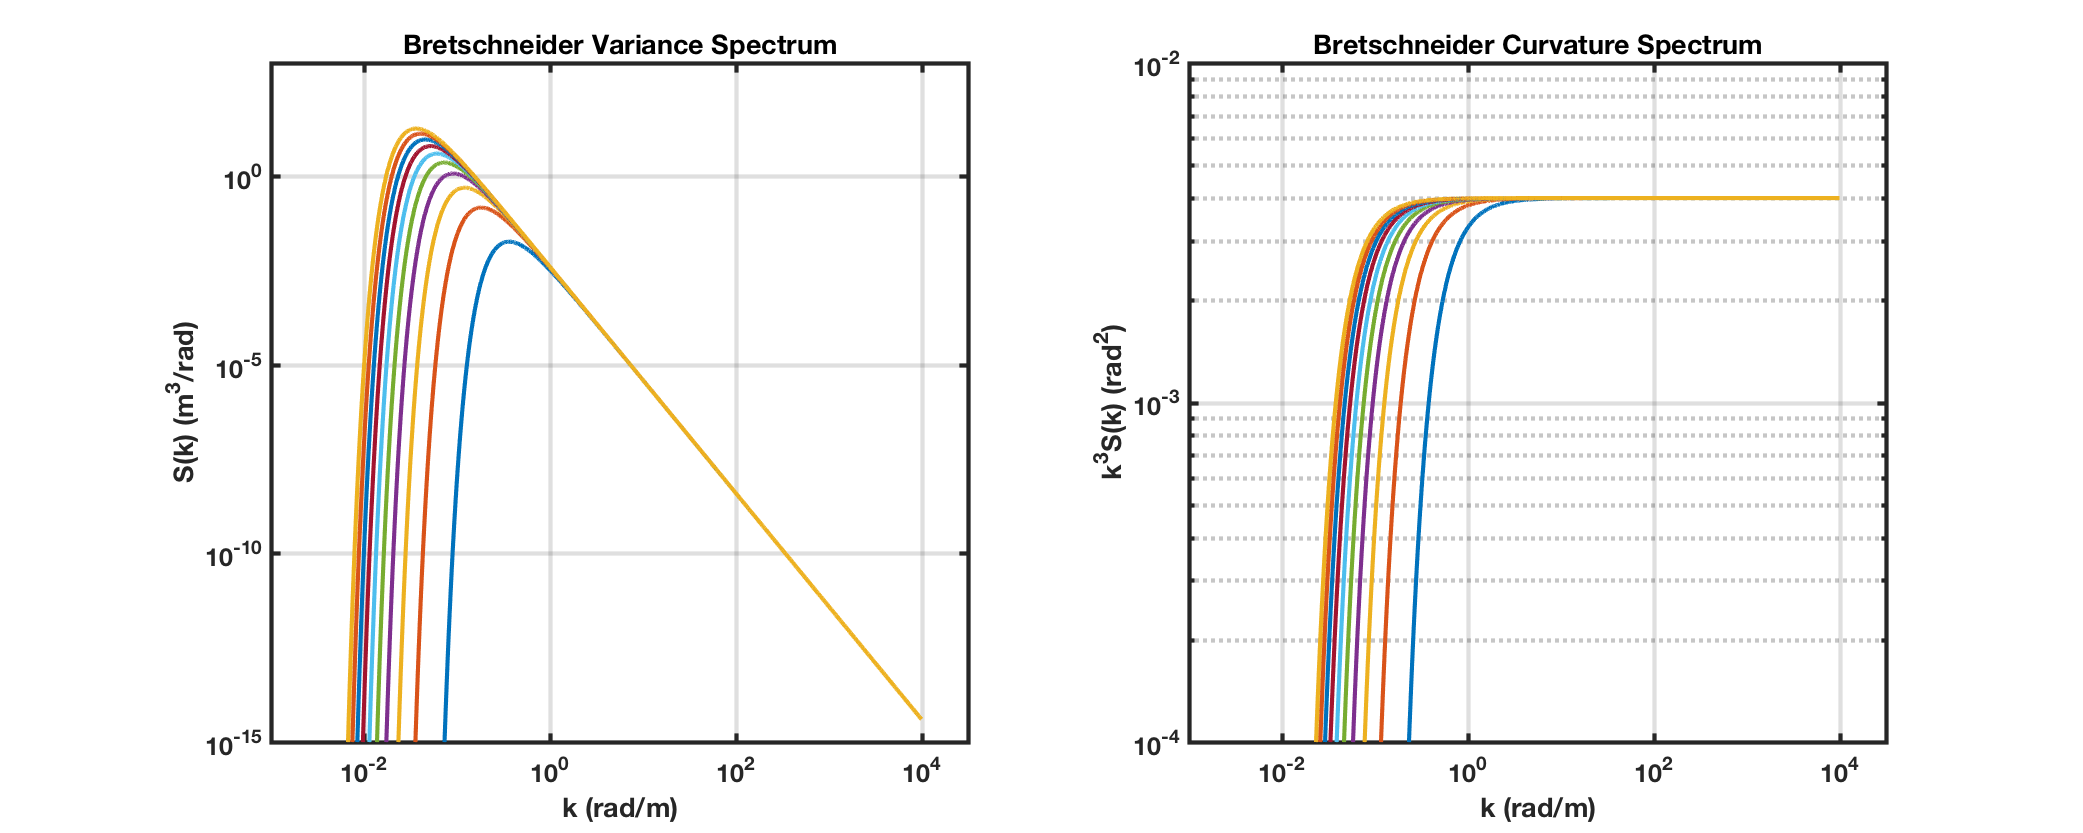
\includegraphics[width=6in]{../media/Ocean_Surface/bs_variance_curvature_spectrum.png}
  \end{center}
  \renewcommand{\baselinestretch}{1} \small\normalsize
  \begin{quote}
    \caption[Bretschneider Variance and Curvature Spectra]{Bretschneider Variance and Curvature Spectra\label{os_fig:1a}}
  \end{quote}
\end{figure}
 \renewcommand{\baselinestretch}{2} \small\normalsize
The Bretschneider spectrum is a two-parameter spectrum as both the exponential term and the amplitude in Equation \ref{os_eq:1a} are dependent on significant wave height.

\subsection{JONSWAP Spectrum}
The Joint North Sea Wave Project (JONSWAP) in the 1970s modified the Pierson-Moskowitz spectrum by adding a peak enhancement factor as shown in Equation \ref{os_eq:1b} \cite{michel_sea_spectra}.
\begin{equation}
  \label{os_eq:1b}
  S(k) = S_{PM}(k)\nu^{\frac{k-k_0}{2\sigma^2k_0}} 
  \end{equation}
The enhancement factor $\nu$ was empirically derived for locations in the North Sea and allows control of the amplitude as in the Bretschneider spectrum. The difference is that the JONSWAP enhancement factor only amplifies the spectrum around the spectral peak.

\subsection{Elfouhaily Spectrum}
Many additional spectra have been developed and in 1997, Elfouhaily et. al extended several of these to provide a unified modern spectrum that is broken into low and high spatial frequency regions, $B_l$ and $B_h$, \cite{elfouhaily}. 

\subsubsection{Spectrum Definition}
The 1-dimensional version of the Elfouhaily spectrum is given in Equation \ref{os_eq:2}.
\begin{equation}
  \label{os_eq:2}
  S(k) = k^{-3}\left[B_l + B_h \right]
\end{equation}
\renewcommand{\baselinestretch}{2} \small\normalsize
This spectrum is dependent on the wind speed at 10 m altitude ($U_{10}$) and the inverse age parameter ($\Omega$). The inverse age parameter indicates how developed the sea is; fully developed for $\Omega = 0.84$, mature for $\Omega = 1.0$, and young for $\Omega > 2.0$. 

The low spatial frequency region, $B_l$, is given by Equation \ref{os_eq:3} and the parameters are defined in Table \ref{os_tab:1} and Equation \ref{os_eq:3a}. Here we are using $v$ to represent phase speed rather than $c$ to prevent confusion with the speed of light.
\begin{equation}
  \label{os_eq:3}
 B_l = \frac{1}{2} \alpha_p \frac{v_p}{v} F_p
\end{equation}
\renewcommand{\baselinestretch}{2} \small\normalsize
\begin{subequations}
\label{os_eq:3a}
   Low spatial frequency spectrum dependencies:
\begin{align}
  F_p &= L_{PM}J_pe^{-\frac{\Omega}{\sqrt{10}}\left[\sqrt{k/_{k_p}} - 1 \right]} &  k_p &= g\left(\frac{\Omega}{U_{10}}\right)^2 & v_p &= \frac{U_{10}}{\Omega} \\
   L_{PM} &=e^{-\frac{5}{4}\left(\frac{k_p}{k} \right)^2} &  J_p &= \gamma^\Gamma  & \alpha_p &= 0.006\Omega^{0.55} 
\end{align}
\end{subequations}
\renewcommand{\baselinestretch}{2} \small\normalsize
\begin{table}[H]
  \begin{center}
      \renewcommand{\baselinestretch}{1} \small\normalsize
  \begin{quote}
    \caption[Elfouhaily Low Spatial Frequency Spectrum Parameters]{Elfouhaily Low Spatial Frequency Spectrum Parameters\label{os_tab:1}}
  \end{quote}
  \begin{tabular} {|c | c |}
    \hline
  \bf{Parameter} & \bf{Description} \\ \hline
  $F_p$ & Long wave side effect function \\ \hline
  $k_p$ &  Wave number of the spectral peak \\ \hline
  $v_p$ &  Phase speed at the spectral peak \\ \hline
  $L_{PM}$ & PM shape spectrum \\ \hline
  $J_p$ & JONSWAP peak enhancement function \\ \hline
  $\alpha_p$ & Generalized Phillips-Kitaigorodskii long wave equilibrium range parameter\\ \hline
  $v$ & Phase speed of the wave \\ \hline
\end{tabular}
\end{center}
\end{table}
\renewcommand{\baselinestretch}{2} \small\normalsize
The high spatial frequency region, $B_h$, is given by Equation \ref{os_eq:4} and the parameters are defined in Table \ref{os_tab:2} and Equations \ref{os_eq:4a} and \ref{os_eq:4b}.
\begin{equation}
  \label{os_eq:4}
 B_h = \frac{1}{2} \alpha_m \frac{v_m}{v} F_m
\end{equation}
\renewcommand{\baselinestretch}{2} \small\normalsize
\begin{subequations}
\label{os_eq:4a}
   High spatial frequency spectrum dependencies:
\begin{align}
  F_m &= L_{PM}J_pe^{-\frac{1}{4}\left[k/_{k_m} - 1 \right]^2 } & k_m & = 370 \text{ rad/m} &  v_m &=\sqrt{\frac{2g}{k_m}} = 0.23 \text{ m/s} \\
  u^* &= \sqrt{Cd_{10N}}U_{10}  & L_{PM} &=e^{-\frac{5}{4}\left(\frac{k_p}{k} \right)^2}  &  J_p &= \gamma^\Gamma
\end{align}
\end{subequations}
\renewcommand{\baselinestretch}{2} \small\normalsize
\begin{equation}
\begin{gathered}
  \label{os_eq:4b}
   \alpha_m= \begin{cases}
    10^{-2}\left[1 + \log\left(\frac{u^*}{v_m} \right) \right],& \text{if } u^* \leq v_m\\
    10^{-2}\left[1 + 3\log\left(\frac{u^*}{v_m} \right) \right], & \text{if } u^* > v_m\\
  \end{cases}
\end{gathered}
\end{equation}
\renewcommand{\baselinestretch}{2} \small\normalsize

\begin{table}[H]
  \begin{center}
      \renewcommand{\baselinestretch}{1} \small\normalsize
  \begin{quote}
    \caption[Elfouhaily High Spatial Frequency Spectrum Parameters]{Elfouhaily High Spatial Frequency Spectrum Parameters\label{os_tab:2}}
  \end{quote}
  \begin{tabular} {|c | c |}
    \hline
  \bf{Parameter} & \bf{Description} \\ \hline
  $F_m$ & Short wave side effect function \\ \hline
  $k_m$ &  Wave number at the secondary peak of the curvature spectrum \\ \hline
  $v_m$ &  Minimum phase speed at $k_m$ \\ \hline
  $\alpha_m$ & Generalized Phillips-Kitaigorodskii short wave equilibrium range parameter \\ \hline
  $L_{PM}$ & PM shape spectrum \\ \hline
  $J_p$ & JONSWAP peak enhancement function \\ \hline
  $Cd_{10N}$ & Neutral stability drag coefficient at 10 m above sea level, $\approx 0.00144$ \\ \hline
  $v$ & Phase speed of the wave \\ \hline
\end{tabular}
\end{center}
\end{table}
\renewcommand{\baselinestretch}{2} \small\normalsize
The variables $L_{PM}$ and $J_p$ are found in both $B_l$ and $B_h$ and are given by Equation \ref{os_eq:5}.
\begin{equation}
\begin{gathered}
  \label{os_eq:5}
    \gamma = \begin{cases}
    1.7,& \text{if } 0.84 < \Omega < 1\\
    1.7 + 6\log{\Omega}, & \text{if } 1 < \Omega < 5
  \end{cases} \\
  \Gamma = \exp{\left[- \frac{\left(\sqrt{\frac{k}{kp} - 1} \right)^2}{2\sigma^2} \right]} \\
  \sigma = 0.08\left[1 + 4\Omega^{-3} \right] \\
\end{gathered}
\end{equation}
\renewcommand{\baselinestretch}{2} \small\normalsize
In \cite{elfouhaily}, the dispersion relation that holds for both gravity and capillary waves is given as 
\begin{equation}
\label{os_eq:5aa}
\omega^2 = gk\left[1 + \left(\frac{k}{k_m}\right)^2 \right]
\end{equation}
We can use Equation \ref{os_eq:5aa} to define the phase speed as
\begin{equation}
\label{os_eq:5ab}
v = \frac{\omega}{k}= \sqrt{\frac{g}{k}\left[1 + \left(\frac{k}{k_m}\right)^2 \right]}
\end{equation}

In the case where we have fetch rather than the inverse age parameter, we can compute the inverse age parameter as shown in Equation \ref{os_eq:5a}. Here $x$ is the dimensional fetch in m and $X$ is the non-dimensional fetch.
\begin{equation}
\label{os_eq:5a}
\begin{gathered}
 X = \frac{g}{U_{10}^2}x\\
 X_0 = 2.2 \times 10^4 \\
 \Omega = 0.84\tanh\left[\left(\frac{X}{X_0} \right)^{0.4} \right]^{-0.75} \\
\end{gathered}
\end{equation}
\renewcommand{\baselinestretch}{2} \small\normalsize

\subsubsection{Spectrum Visualization}
The variance power spectrum is shown in the left hand side of Figure \ref{os_fig:3} and the associated curvature spectrum is shown in the right hand side of Figure \ref{os_fig:3}. These figures were generated for wind speeds from 3 m/s to 21 m/s in increments of 2 m/s, matching Figure 8 in \cite{elfouhaily}. In these figures, the secondary peak can clearly be seen at 370 rad/m.
\begin{figure}[H]
  \begin{center}
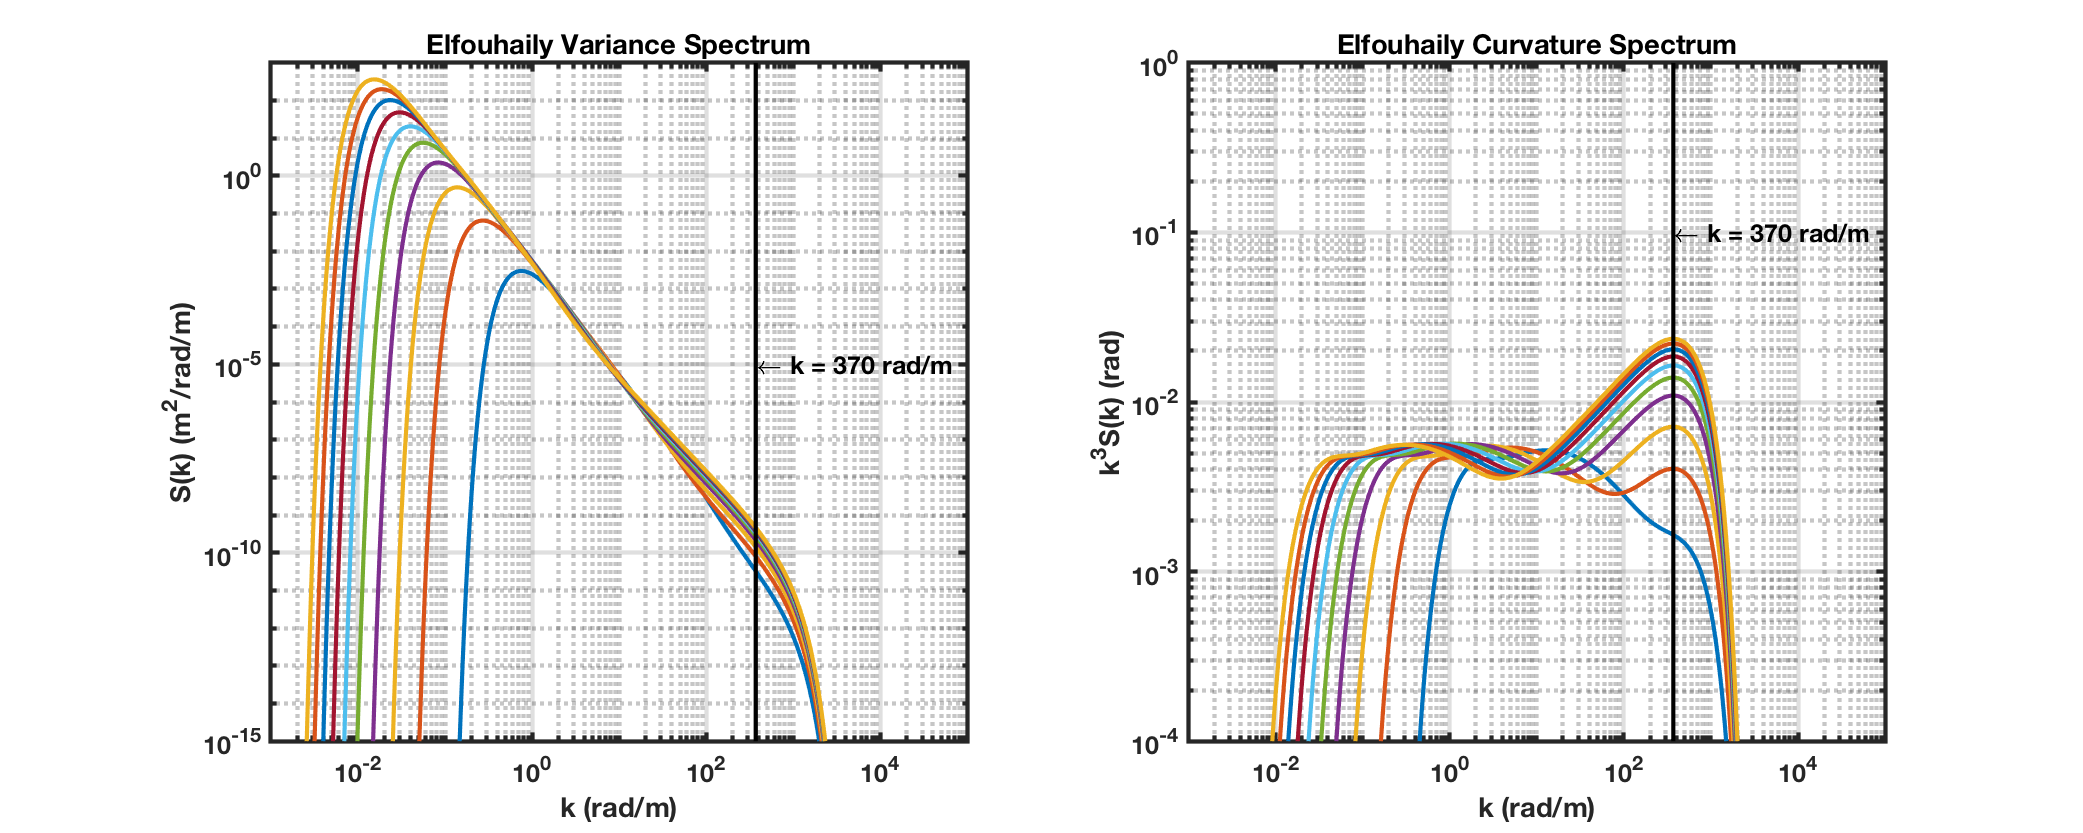
\includegraphics[width=6in]{../media/Ocean_Surface/elf_variance_curvature_spectrum.png}
  \end{center}
  \renewcommand{\baselinestretch}{1} \small\normalsize
  \begin{quote}
    \caption[Elfouhaily Variance and Curvature Spectra vs. $U_{10}$]{Elfouhaily Variance and Curvature Spectra vs. $U_{10}$\label{os_fig:3}}
  \end{quote}
\end{figure}
\renewcommand{\baselinestretch}{2} \small\normalsize

To demonstrate the impact from the inverse age parameter, the variance power spectrum is shown in the left hand side of Figure \ref{os_fig:3a} and the associated curvature spectrum is shown in the right hand side of Figure \ref{os_fig:3a}. These figures were generated for $\Omega$ ranging from $0.84$ (fully developed) to $5.0$ (very young). From this figure, we can see that the spectra show energy transferring from high spatial frequencies to low spatial frequencies and the spectral peak flattening as the sea develops.
\begin{figure}[H]
  \begin{center}
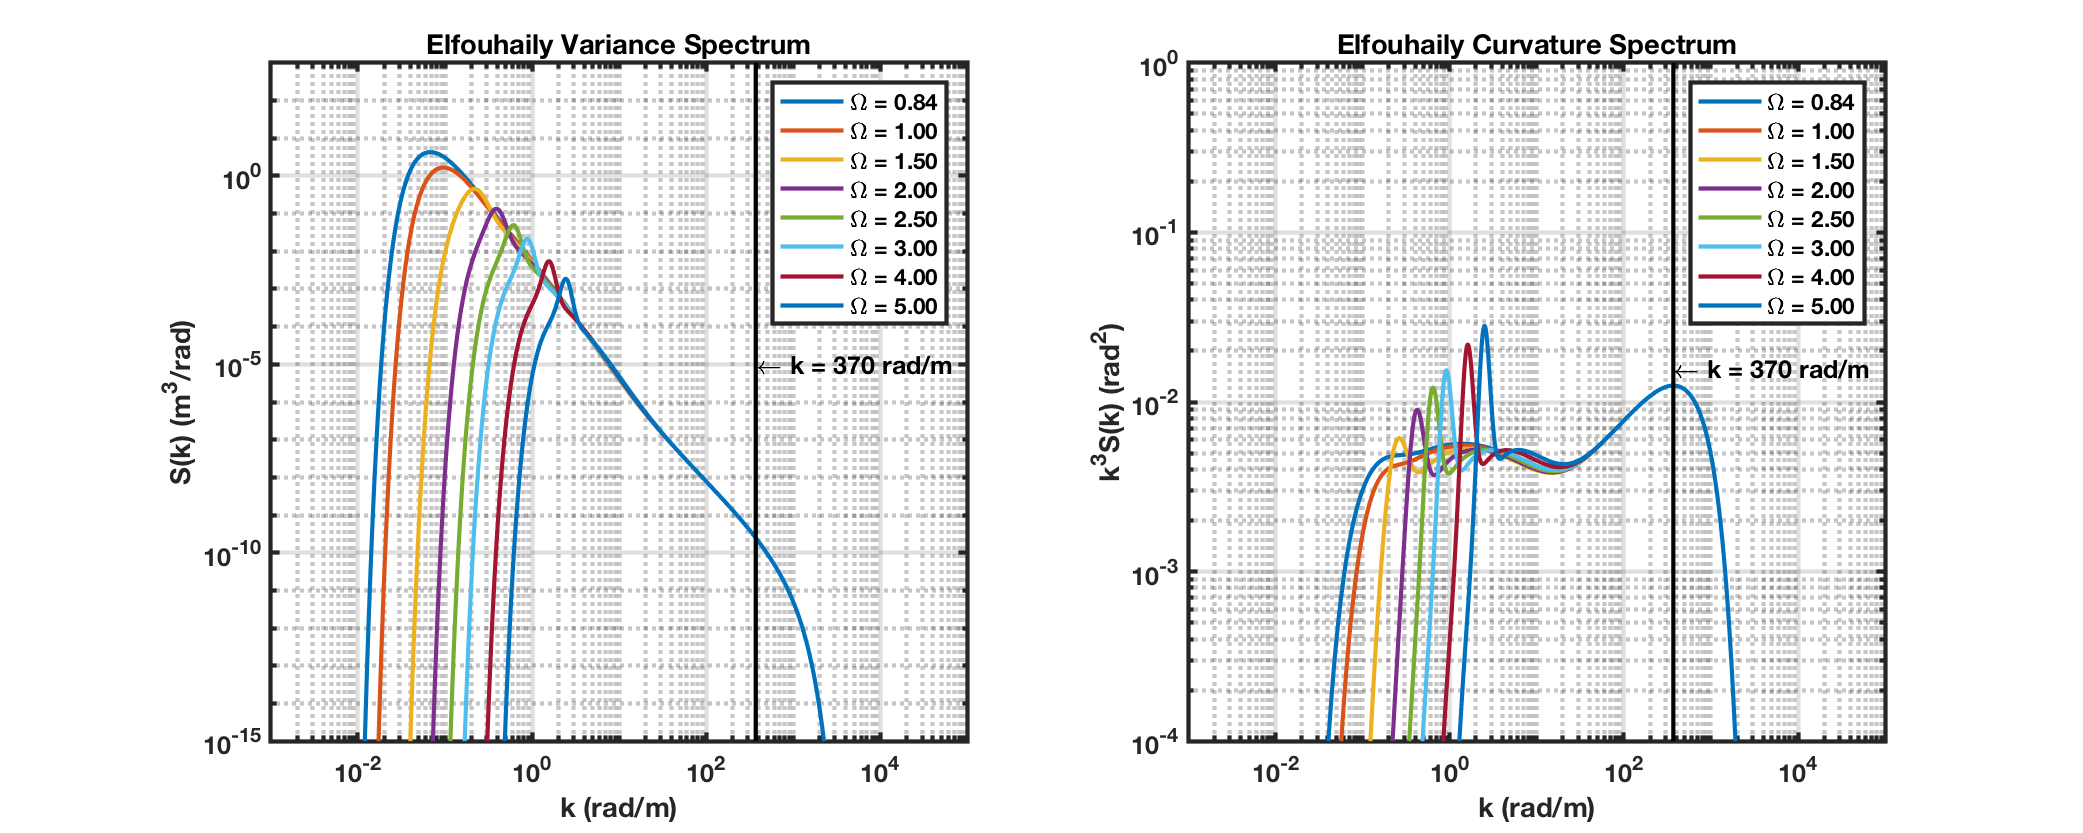
\includegraphics[width=6in]{../media/Ocean_Surface/elf_variance_curvature_spectrum_age.png}
  \end{center}
  \renewcommand{\baselinestretch}{1} \small\normalsize
  \begin{quote}
    \caption[Elfouhaily Variance and Curvature Spectra vs. $\Omega$]{Elfouhaily Variance and Curvature Spectra vs. $\Omega$ \label{os_fig:3a}}
  \end{quote}
\end{figure}
\renewcommand{\baselinestretch}{2} \small\normalsize

\subsubsection{Comparison with PM Spectrum}
To compare the results, the Elfouhaily and PM variance power spectra are shown in the left hand side of Figure \ref{os_fig:2} for wind speeds of 5 m/s and 10 m/s. The inverse age parameter was set to 0.84 to match and the wind speed at 19 m altitude was approximated as $U_{19} \approx 1.026 U_{10}$. The Elfouhaily spectra are shown by the dashed lines and indicate a deviation from the PM spectra at large wave numbers. The corresponding curvature spectra are shown in the right hand side of Figure \ref{os_fig:2}. 
\begin{figure}[H]
  \begin{center}
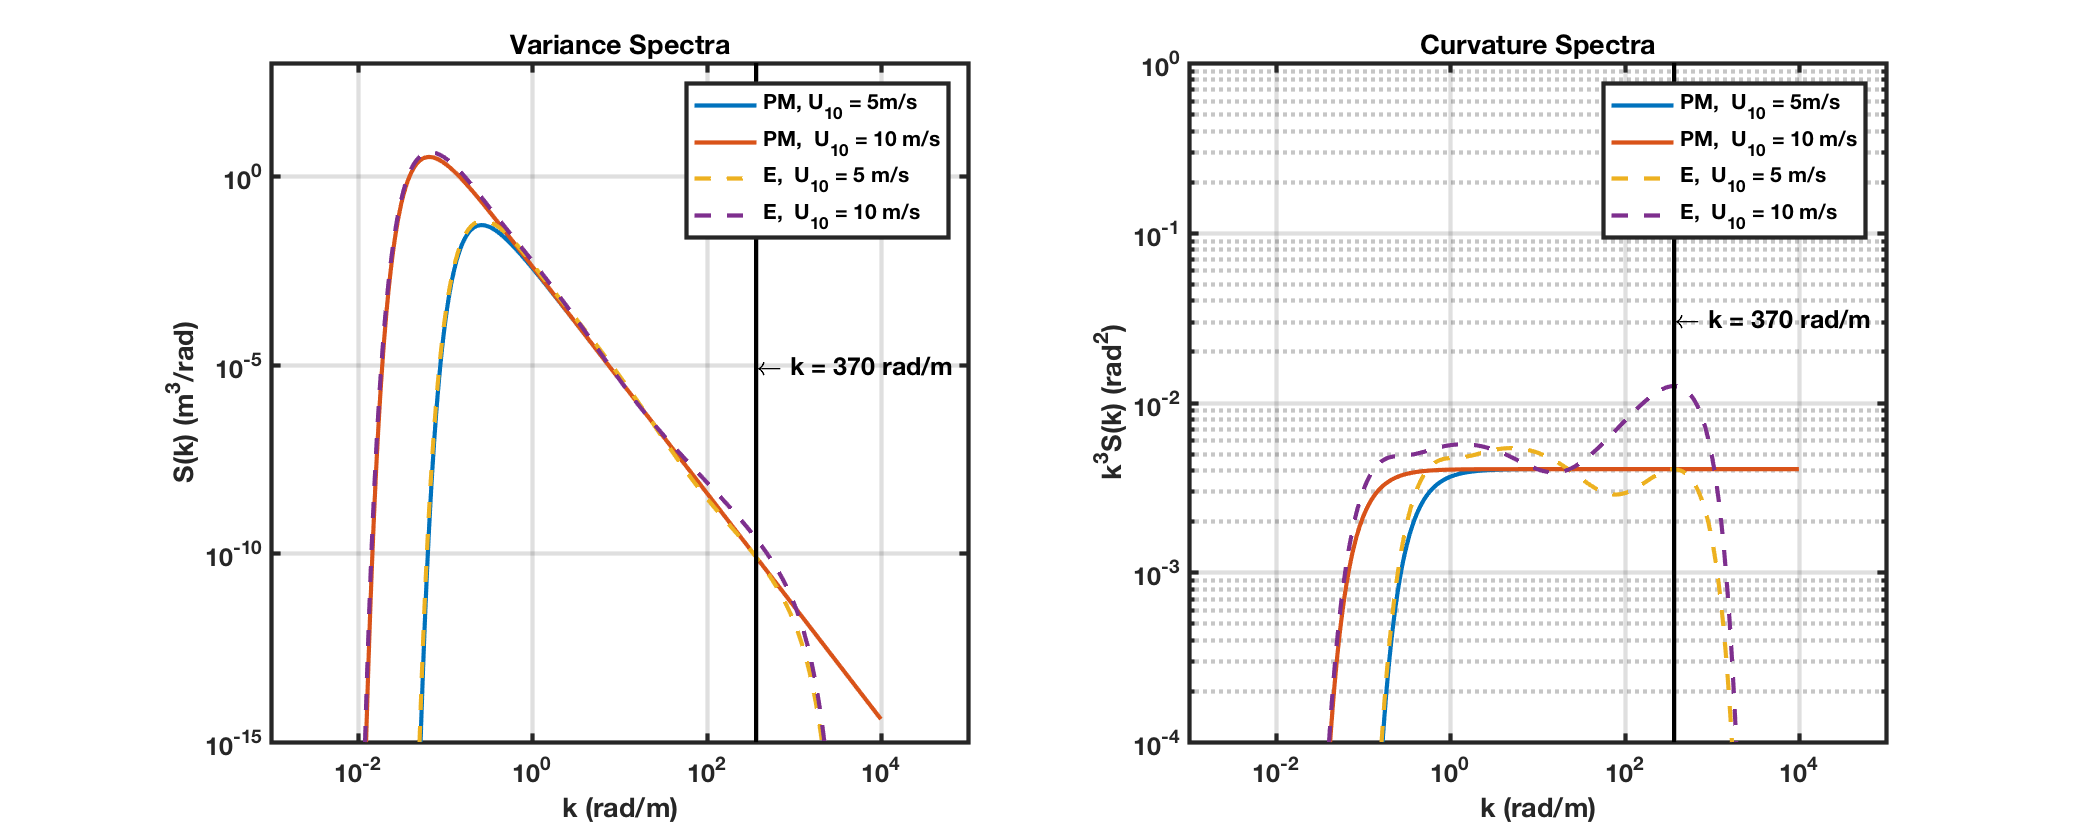
\includegraphics[width=6in]{../media/Ocean_Surface/elf_vs_PM_variance_curvature_spectrum.png}
  \end{center}
  \renewcommand{\baselinestretch}{1} \small\normalsize
  \begin{quote}
    \caption[Elfouhaily vs. Pierson Moskowitz Variance and Curvature Spectra]{Elfouhaily vs. Pierson Moskowitz Variance and Curvature Spectra\label{os_fig:2}}
  \end{quote}
\end{figure}
\renewcommand{\baselinestretch}{2} \small\normalsize

\subsection{Directional Spreading Functions}
All the variance power spectra that have been discussed are uni-directional, meaning they only apply downrange in the direction of the wind. For two-dimensional surfaces, we need to include angular extent. This can be accomplished by applying a spreading function $\Phi$ in $k$-space as shown in Equation \ref{os_eq:5b} \cite{elfouhaily}.
\begin{equation}
\label{os_eq:5b}
\Psi(k,\phi) = \frac{1}{k}S(k)\Phi(k,\phi)
\end{equation}
\renewcommand{\baselinestretch}{2} \small\normalsize
As discussed in \cite{elfouhaily}, the spreading function should be symmetric in upwind-crosswind and will have the form given in Equation \ref{os_eq:5c}.
\begin{equation}
\label{os_eq:5c}
\Psi(k,\phi) = \frac{1}{2\pi}\left[1 + \Delta(k)\cos(2\phi) \right]
\end{equation}
\renewcommand{\baselinestretch}{2} \small\normalsize

Here $\Delta(k)$ is defined as in Equation \ref{os_eq:5d}.
\begin{equation}
\label{os_eq:5d}
\begin{gathered}
\Delta(k) = \tanh\left( a_0 + a_p\left(\frac{v}{v_p}\right)^{2.5}  + a_m\left(\frac{v_m}{v} \right)^{2.5}\right)\\
a_0 = \frac{\log(2)}{4} \\
a_p = 4\\
a_m = 0.13\frac{u^*}{v_m} \\
\end{gathered}
\end{equation}
\renewcommand{\baselinestretch}{2} \small\normalsize

The complete 2-dimensional unified Elfouhaily spectrum is given in Equation \ref{os_eq:5e}.
\begin{equation}
\label{os_eq:5e}
\boxed{\Psi(k,\phi) = \frac{1}{2\pi k^4}\left[B_l + B_h \right] \left[1 + \Delta(k)\cos(2\phi) \right]}
\end{equation}

Figure \ref{os_fig:7bb} shows the 2-D variance and curvature power spectra on a log scale. In the curvature spectrum, we can see the secondary peak as in the 1-dimensional case.
\begin{figure}[H]
  \begin{center}
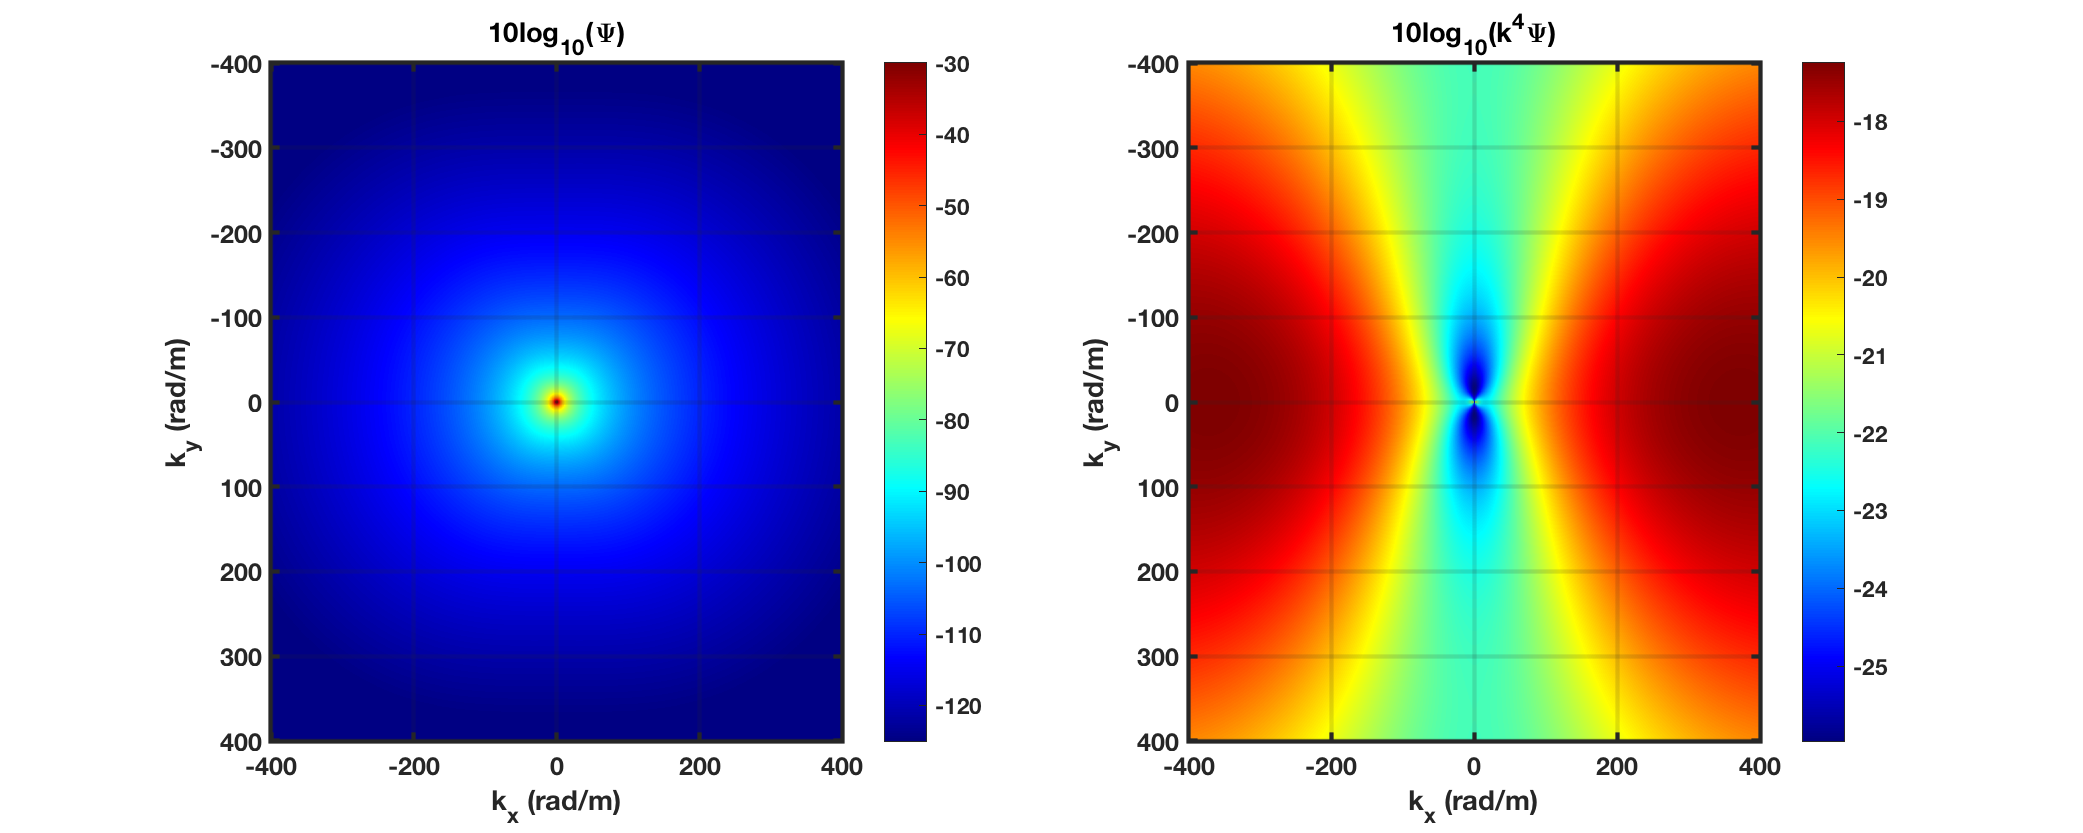
\includegraphics[width=6in]{../media/Ocean_Surface/elf_variance_curvature_spectrum_2D.png}
  \end{center}
  \renewcommand{\baselinestretch}{1} \small\normalsize
  \begin{quote}
    \caption[Elfouhaily 2-D Variance and Curvature Power Spectra]{Elfouhaily 2-D Variance and Curvature Power Spectra\label{os_fig:7bb}}
  \end{quote}
\end{figure}
\renewcommand{\baselinestretch}{2} \small\normalsize

Figure \ref{os_fig:7cc} shows the low frequency behavior of the 2-D variance power spectrum.
\begin{figure}[H]
  \begin{center}
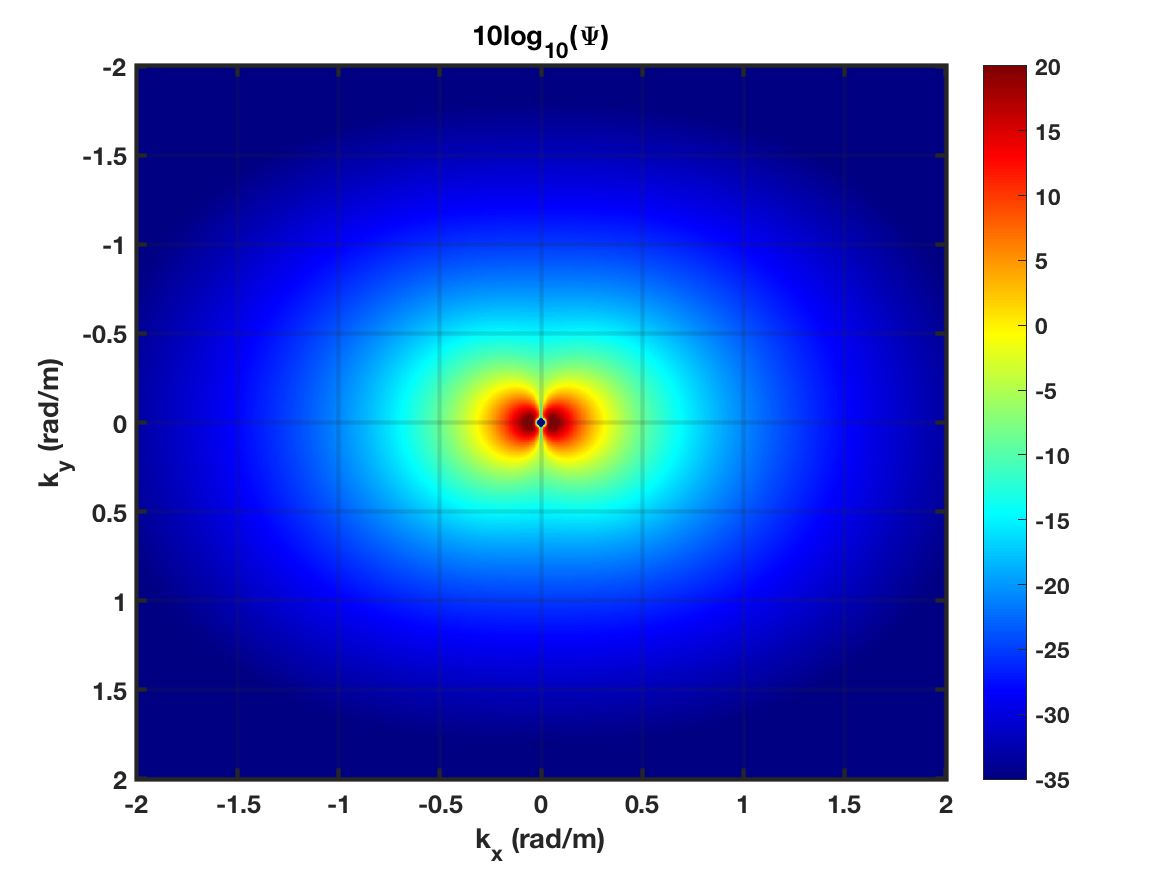
\includegraphics[width=4in]{../media/Ocean_Surface/elf_variance_spectrum_2D_zoom.png}
  \end{center}
  \renewcommand{\baselinestretch}{1} \small\normalsize
  \begin{quote}
    \caption[Elfouhaily 2-D Variance Power Spectrum]{Elfouhaily 2-D Variance Power Spectrum\label{os_fig:7cc}}
  \end{quote}
\end{figure}
\renewcommand{\baselinestretch}{2} \small\normalsize

\section{Generation of Sea Surface Realizations in 1-Dimension}\label{os_sec:1d}
Realizations of sea surfaces rely on having adequate sampling to cover both the spectral and spatial ranges of interest and then generating an appropriate set of Fourier coefficients. The 1-dimensional case is easiest to both understand and implement and will be discussed first.

\subsection{Sampling Constraints}\label{os_label:1d_sampling_constraints}
In order to generate a random sea surface, we need to establish the number of points to use ($N$) and the spatial domain length to cover ($L$). The spatial domain sampling inteval is then $\Delta x = \frac{L}{N}$ and the frequency domain sampling interval is $\Delta k = \frac{2\pi}{L}$. 

From the Nyquist sampling theorem, the highest wave number that can be sampled given these values is $k_{max} = \frac{N}{2}\Delta k = \frac{N\pi}{L}$ rad/m, which corresponds to a minimum wavelength of $\lambda_{min} = 2\Delta x = \frac{2L}{N}$ m.

Immediately, we see that to cover up to the secondary peak at $k_m$, $\frac{N}{L}\pi > k_m$ or $N > \frac{k_m}{\pi}L$. Since $k_m = 370$ rad/m, we can round up to state that $N \geq 118L$. In other words, the number of points required to cover up to the secondary peak in the spectrum is 118 times more than the length of the spatial domain. For the 1-dimensional case, this is not too bad as a 10 km length can be sampled with 1,180,000 points. It is in the 2-dimensional case where this really becomes problematic, as we now need $N^2$ points.

Figure \ref{os_fig:6aa} shows the impact on wavenumber sampling for various values of $N$ for $L$ = 1 km. The upper left hand plot shows the case where $N = 5L$, the upper right hand plot shows the case where $N = 10L$, the lower left hand plot shows the case where $N = 118L$, and the lower right hand plot shows the case where $N = 500L$. Since $\Delta x = \frac{L}{N}$, these cases represent spatial resolutions of 1/5 m, 1/10 m, 1/118 m, and 1/500 m. 
\begin{figure}[H]
  \begin{center}
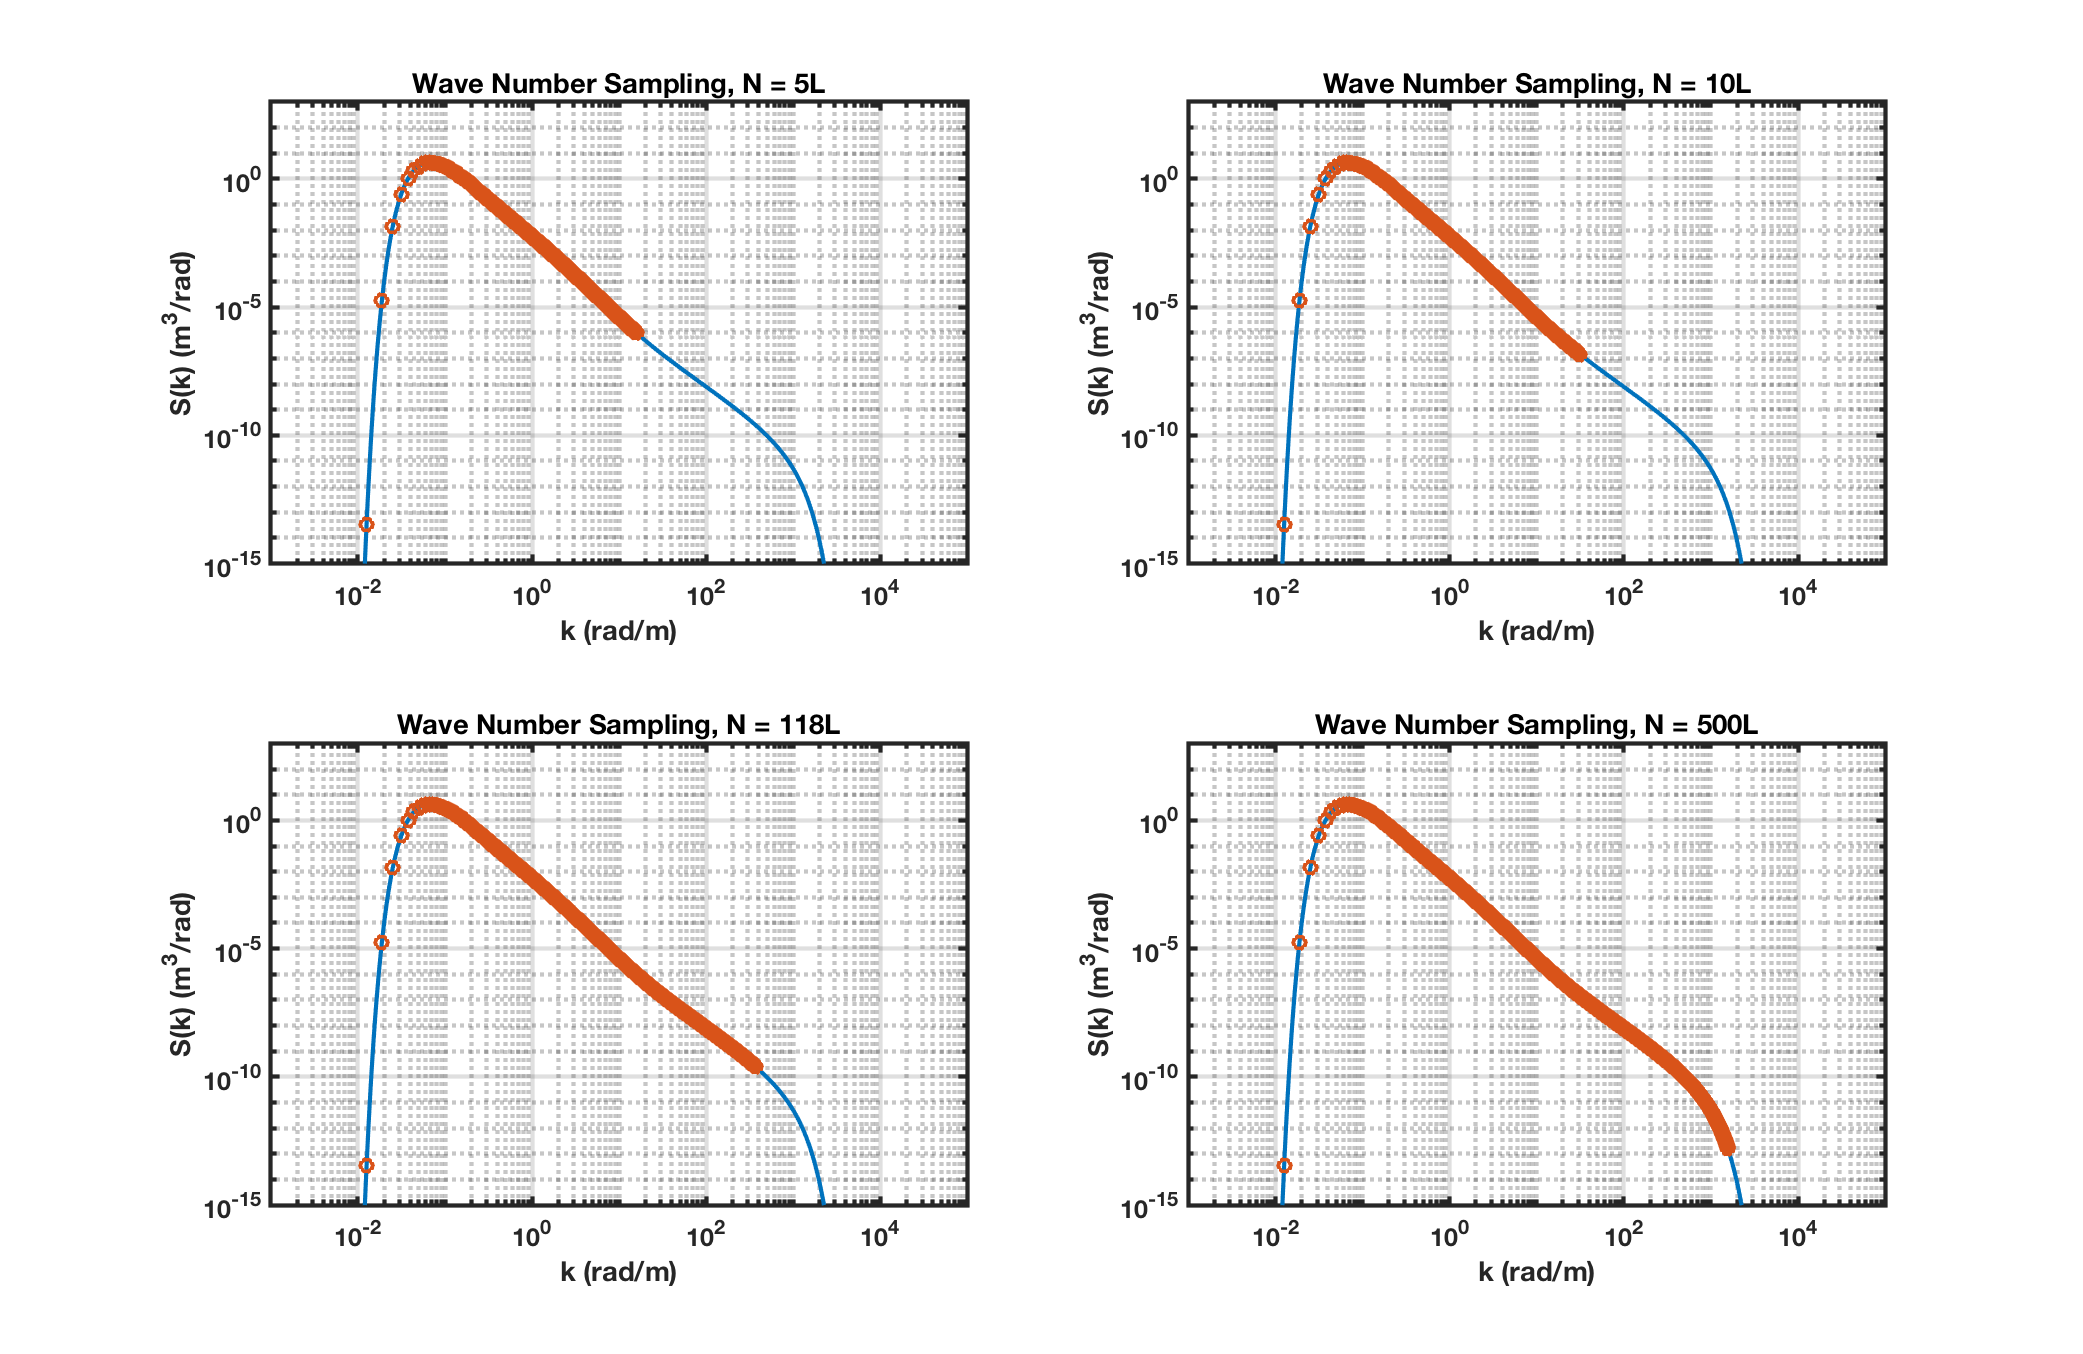
\includegraphics[width=6in]{../media/Ocean_Surface/sampling_coverage.png}
  \end{center}
  \renewcommand{\baselinestretch}{1} \small\normalsize
  \begin{quote}
    \caption[Wavenumber Sampling Coverage]{Wavenumber Sampling Coverage\label{os_fig:6aa}}
  \end{quote}
\end{figure}
\renewcommand{\baselinestretch}{2} \small\normalsize
Since $L$ is the same for each case, $\Delta k$ is also the same and we can see how increasing $N$ increases coverage of higher spatial frequencies.

In many situations, we are not concerned with capturing the high spatial frequencies as much as we are with staying below a pre-defined maximum spatial step. This step is typically on the order of 0.5 m, in which case $N = 2L$.

As a final note for sampling constraints, we need to maintain integer indexing for digital implementation so $N$ must be an even integer to allow the element $N/2$ to be an integer as well. We will define the range in $k$-space as running from $-\left(\frac{N}{2}-1\right)\Delta k$ to $\frac{N}{2}\Delta k$.

\subsection{Frequency Domain Representation}
The general idea is to use the power spectrum to create a realization of the sea surface in the frequency domain and then transform that to the spatial domain through an inverse Fourier transform. We will follow the procedure outlined in \cite{percival_spectra}, 
but we need to provide some additional scale factors to account for conservation of energy.

To handle discretization of the power spectrum, we use the fact that the amount of energy contained per unit interval is a constant, so that $S(k)dk = S(\omega) d\omega$. To normalize the spectrum to the specified wave number sampling interval, we simply need to multiply by $\Delta k$. Next, since we have a one-sided spectrum rather than a two-sided one, we only have half the energy present and need to divide the power spectrum by 2. With these factors included, we can define the one-sided, discrete spectrum as $S_d = \frac{S(k)\Delta k}{2}$.

To generate the frequency domain representation ($V_j$), we will take a set of Gaussian distributed random variables that are scaled  by the square root of the power spectrum and arrange them so the sequence is Hermitian, $V(k) = V^*(-k)$. Because $N$ is even, as described in Section \ref{os_label:1d_sampling_constraints}, there are special cases to handle to ensure that the sequence is Hermitian. $V_j$ only contains a single element for $k = 0$ and $k = \frac{N}{2}\Delta k$ and must be purely real at both frequencies. If we take a pair of uncorrelated Gaussian distributed random variables of length $\frac{N}{2}$ ($w$ and $u$), we can generate $V_j$ as shown in Equation \ref{os_eq:8}.

\begin{equation}
  \label{os_eq:8}   
  V_j = \begin{cases}
    \sqrt{\frac{1}{2}S_0\Delta k}w_0, & j = 0 \\
    \frac{1}{2}\sqrt{\frac{1}{2}S_j\Delta k}\left(w_j + iu_j \right), & 1 \leq j < \frac{N}{2} \\
   \sqrt{\frac{1}{2}S_{N/2}\Delta k}u_0 & j = \frac{N}{2} \\
    V_{N-j}^*, &  \frac{N}{2} < j \leq N-1 
  \end{cases} 
\end{equation}
The extra factor of $\frac{1}{2}$ in line 2 of Equation \ref{os_eq:8} comes from the fact that we need to normalize both the expectations $\left<w_j + iu_j\right>$ and $\left<w_j - iu_j\right>$ to conserve energy.

The index ordering is assumed to have $k=0$ at the first element so that the sequence will wrap in frequency at $j = \frac{N}{2} + 1$. An example sequence for $N = 8$ is shown in Table \ref{os_tab:2a}.
\begin{table}[H]
  \begin{center}
      \renewcommand{\baselinestretch}{1} \small\normalsize
  \begin{quote}
    \caption[Example 1-D Hermitian Sequence]{Example 1-D Hermitian Sequence\label{os_tab:2a}}
  \end{quote}
  \begin{tabular} {| c | c | c |}
    \hline
  \bf{$j$} & \bf{$k_j$} & \bf{$V_j$} \\ \hline
  $0$ & $0$ & $\sqrt{\frac{S_{0}}{2} \Delta k}w_0$ \\ \hline
  $1$ & $\Delta k$ & $\frac{1}{2}\sqrt{\frac{S_{1}}{2} \Delta k} \left(w_1 + iu_1 \right)$ \\ \hline
  $2$ & $2\Delta k$ & $\frac{1}{2}\sqrt{\frac{S_{2}}{2} \Delta k} \left(w_2 + iu_2 \right)$ \\ \hline
  $3$ & $3\Delta k$ & $\frac{1}{2}\sqrt{\frac{S_{3}}{2} \Delta k} \left(w_3 + iu_3 \right)$ \\ \hline
  $4$ & $4\Delta k$ & $\sqrt{\frac{S_{4}}{2} \Delta k} u_0$ \\ \hline
  $5$ & $-3\Delta k$ & $\frac{1}{2}\sqrt{\frac{S_{3}}{2} \Delta k} \left(w_3 - iu_3 \right)$ \\ \hline
  $6$ & $-2\Delta k$ & $\frac{1}{2}\sqrt{\frac{S_{2}}{2} \Delta k} \left(w_2 - iu_2 \right)$  \\ \hline
  $7$ & $-\Delta k$ & $\frac{1}{2}\sqrt{\frac{S_{1}}{2} \Delta k} \left(w_1 - iu_1 \right)$ \\ \hline

\end{tabular}
\end{center}
\end{table}
\renewcommand{\baselinestretch}{2} \small\normalsize

Now that we have the random Fourier coefficients, we can generate the sea surface through the inverse Fourier transform as in Equation \ref{os_eq:9}. Because the sequence is Hermitian, the sea surface will be purely real.
\begin{equation}
  \label{os_eq:9}
  h(x) = \mathcal{F}^{-1}\left\{V(k) \right\}
  \end{equation}

\subsection{Example Realizations}
Figure \ref{os_fig:7a} shows an example realization for $U_{10}$ = 10 m/s and $L$ = 1km. The upper plots show the generated sea surface, and a comparison of the original spectrum to the recovered spectrum for $N = 2^{17}$. Here, $N = 131.07L$ and $\Delta x$ = 7.6 mm. The bottom plots show the same for $N=2^{11}$. Here, $N = 2.04L$ and $\Delta x$ = 0.49 m.
\begin{figure}[H]
  \begin{center}
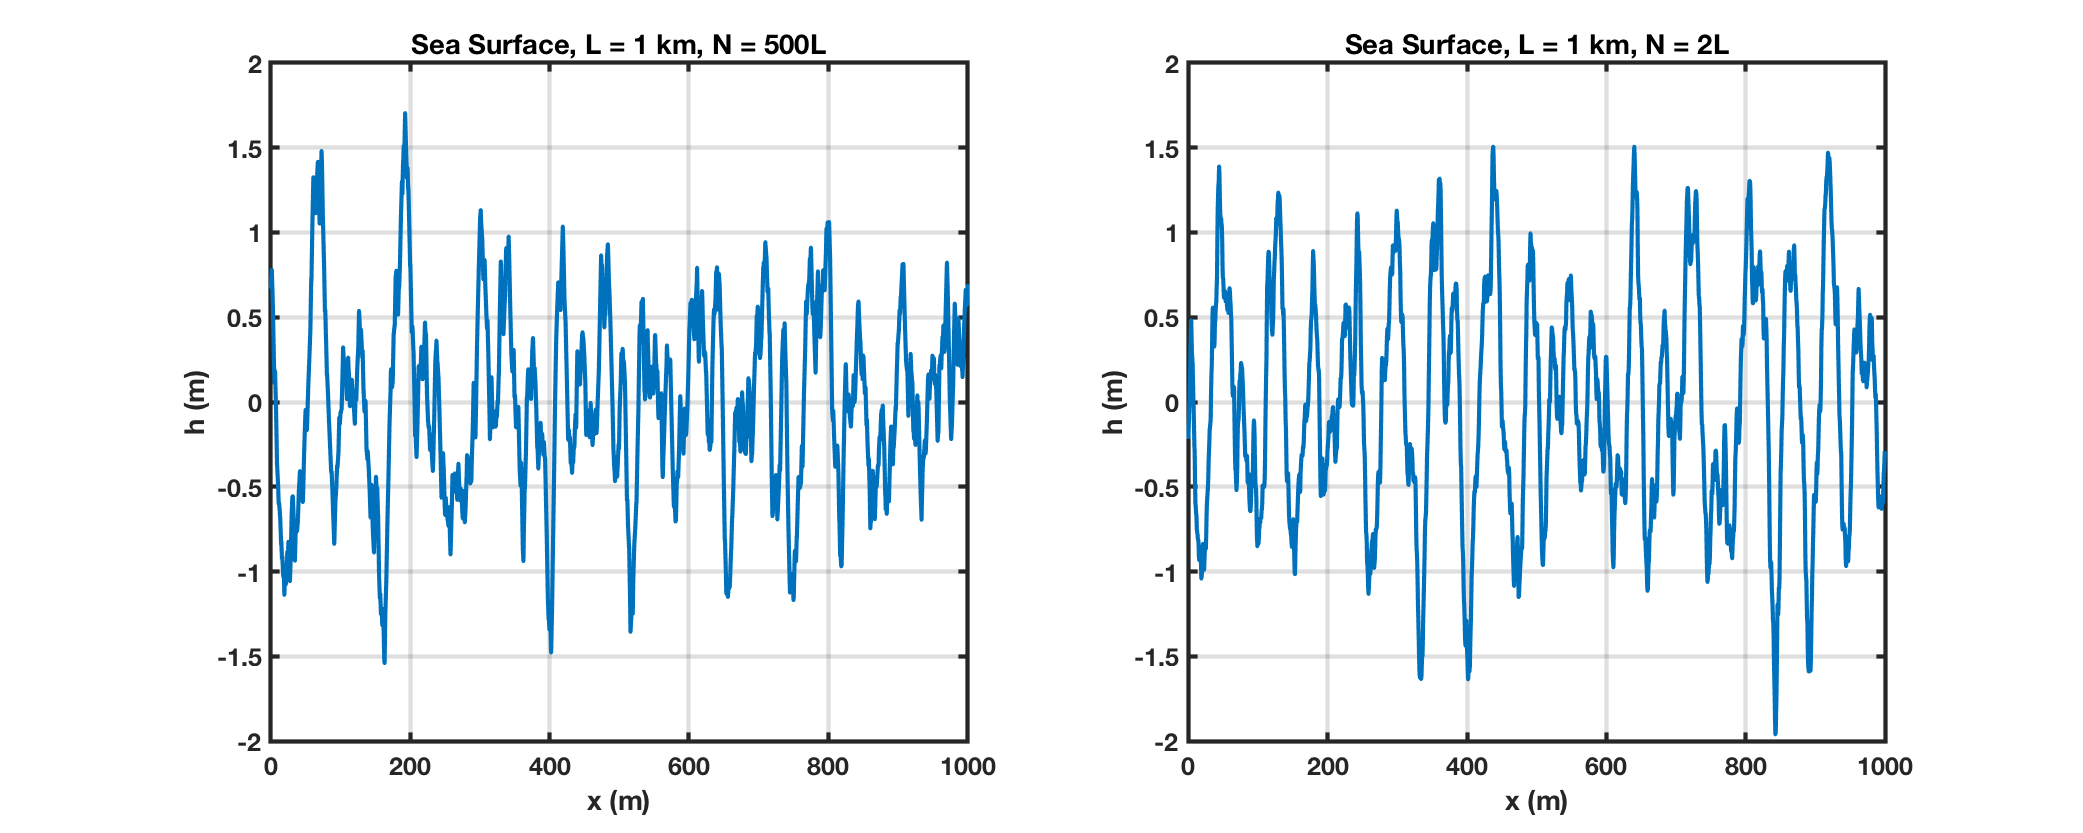
\includegraphics[width=6in]{../media/Ocean_Surface/sea_surface_1000.png}
  \end{center}
  \renewcommand{\baselinestretch}{1} \small\normalsize
  \begin{quote}
    \caption[Example Sea Surface Realization for 1 km Range]{Example Sea Surface Realization for 1 km Range\label{os_fig:7a}}
  \end{quote}
\end{figure}
\renewcommand{\baselinestretch}{2} \small\normalsize

Figure \ref{os_fig:7aa} shows another example realization, this time for $L$ = 10km. The upper plots show the generated sea surface, and a comparison of the original spectrum to the recovered spectrum for $N = 2^{21}$. Here, $N = 209.7L$ and $\Delta x$ = 4.8 mm. The bottom plots show the same for $N=2^{15}$. Here, $N = 3.3L$ and $\Delta x$ = 0.3 m.
\begin{figure}[H]
  \begin{center}
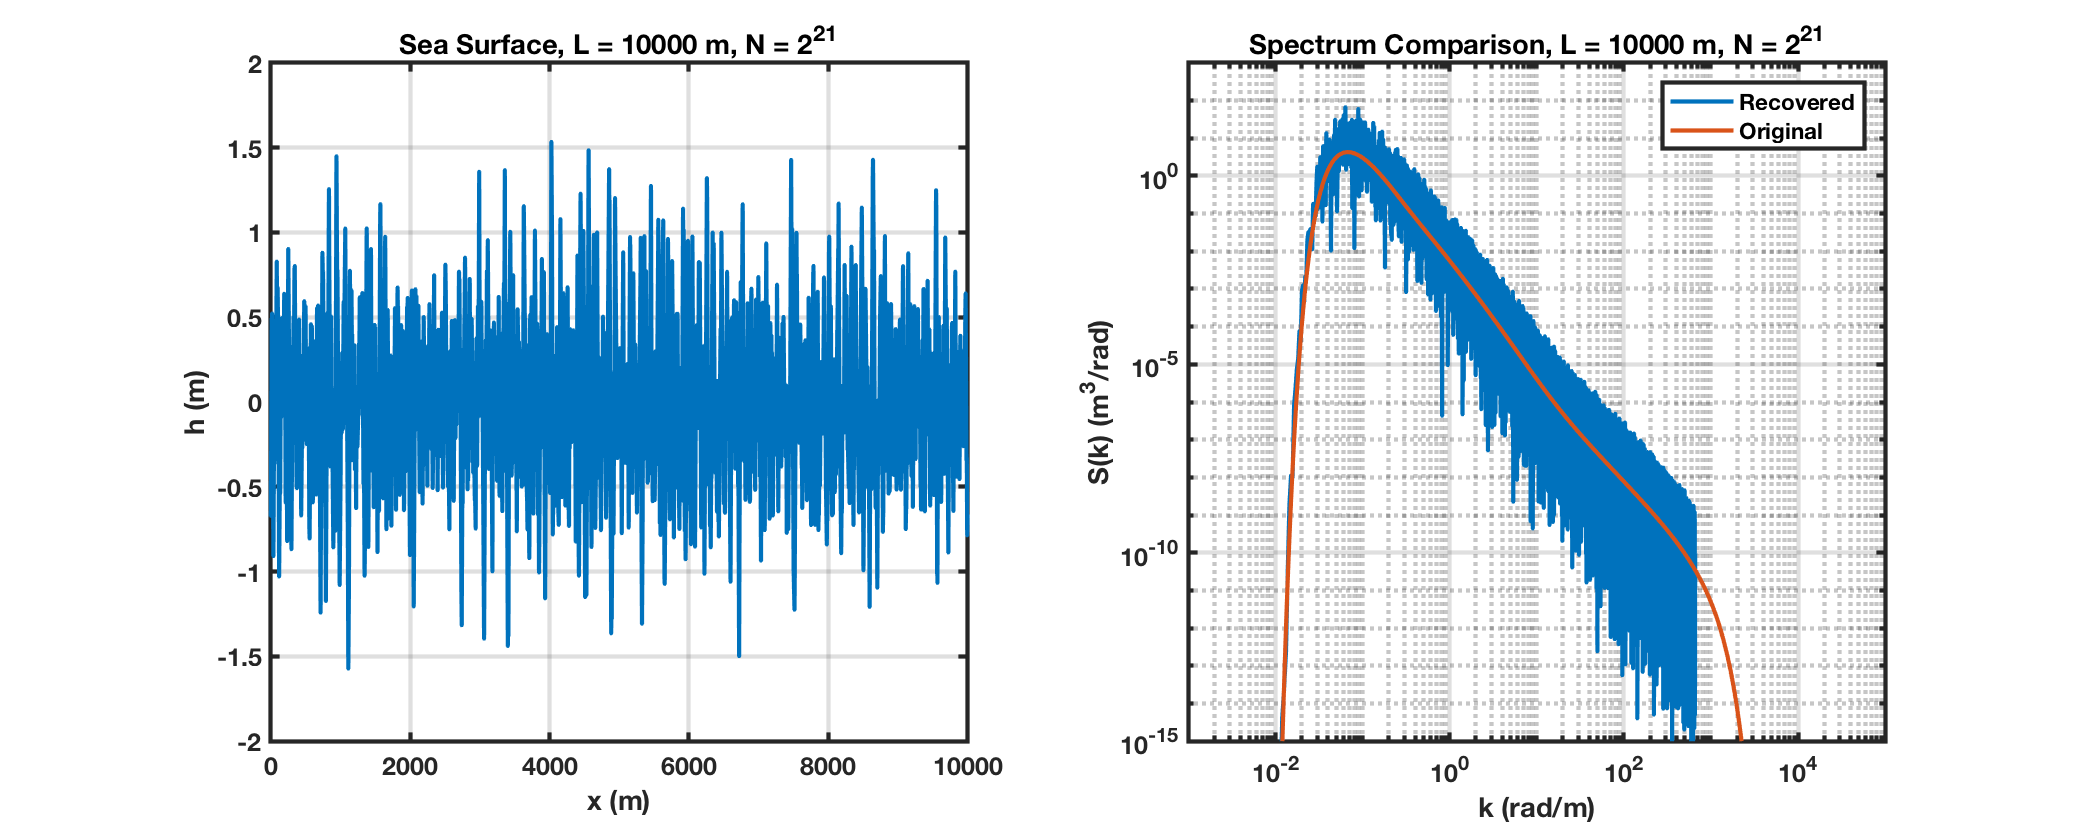
\includegraphics[width=6in]{../media/Ocean_Surface/sea_surface_10000.png}
  \end{center}
  \renewcommand{\baselinestretch}{1} \small\normalsize
  \begin{quote}
    \caption[Example Sea Surface Realization for 10 km Range]{Example Sea Surface Realization for 10 km Range\label{os_fig:7aa}}
  \end{quote}
\end{figure}
\renewcommand{\baselinestretch}{2} \small\normalsize
For both Figures \ref{os_fig:7a} and \ref{os_fig:7aa}, $N$ was set to the next highest power of 2 to capture the secondary peak.

\section{Generation of Sea Surface Realizations in 2-Dimensions}
We will generally follow Section \ref{os_sec:1d} to generate 2-dimensional surfaces but we now have a wave vector $\mathbf{k} = k_x\hat{x} + k_y\hat{y}$ instead of a scalar wave number. In this case we will have matrices and the number of points will go as $N^2$. We still have the constraint that the frequency domain representation should exhibit Hermitian symmetry, so $V(n,m) = V^*(N-n,N-m)$. The special cases at the elements $k = 0$ and $k = \frac{N}{2}$ now turn into special cases for the vectors $k_x = 0$, $k_x = \frac{N}{2}$, $k_y = 0$, and $k_y = \frac{N}{2}$. 

Figure \ref{os_fig:8} shows a section of a generated 2D sea surface. The total surface was $1000 m^2$, only $100 m^2$ is shown here.
\begin{figure}[H]
  \begin{center}
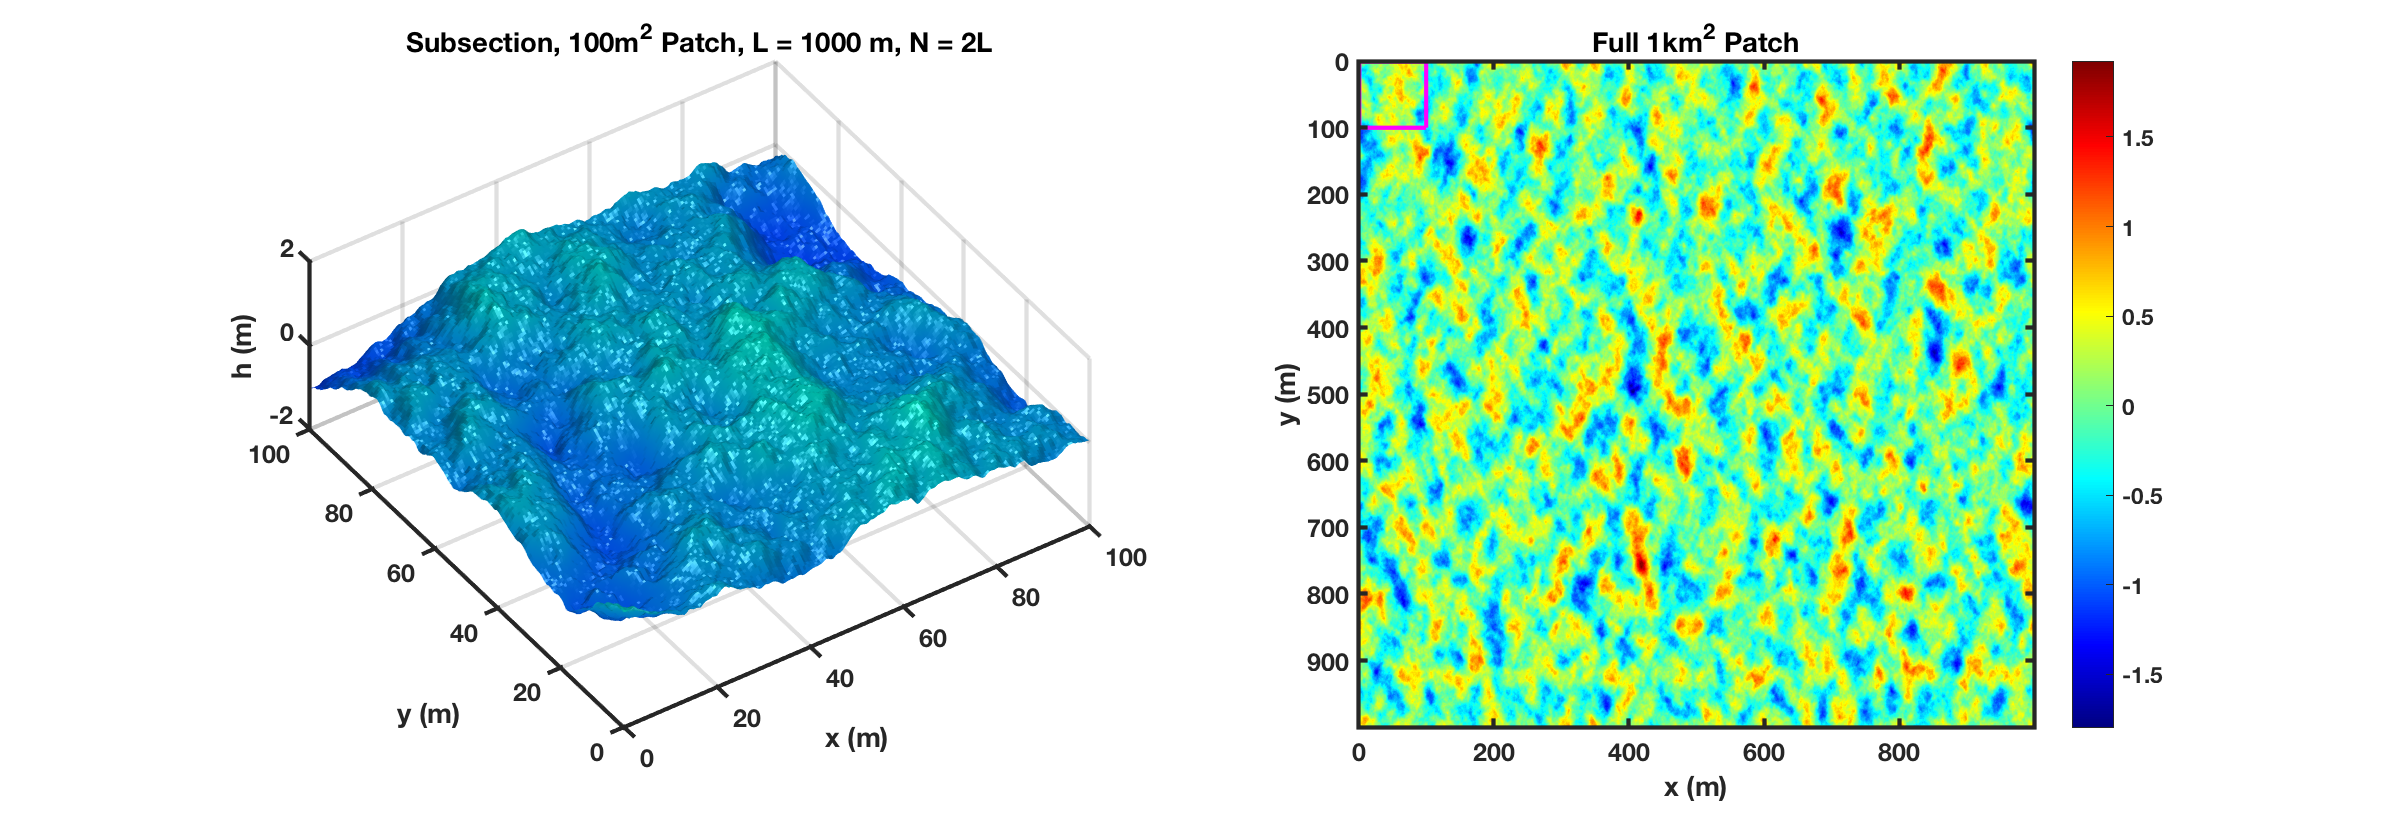
\includegraphics[width=6in]{../media/Ocean_Surface/sea_surface_2d_surf.png}
  \end{center}
  \renewcommand{\baselinestretch}{1} \small\normalsize
  \begin{quote}
    \caption[Generated 2D Sea Surface]{Generated 2D Sea Surface \label{os_fig:8}}
  \end{quote}
\end{figure}
\renewcommand{\baselinestretch}{2} \small\normalsize

Figure \ref{os_fig:10} shows slices along the $N/2$ element in both the $x$ and $y$ planes along with a comparison of the 1D Elfouhaily spectrum to the spectrum recovered from the slices. The low frequency content does not match as well as in the 1-dimensional case. Because we have added a spreading function, we do not expect the crosswind ($y$) slice to match as well as the downwind ($x$) slice.
\begin{figure}[H]
  \begin{center}
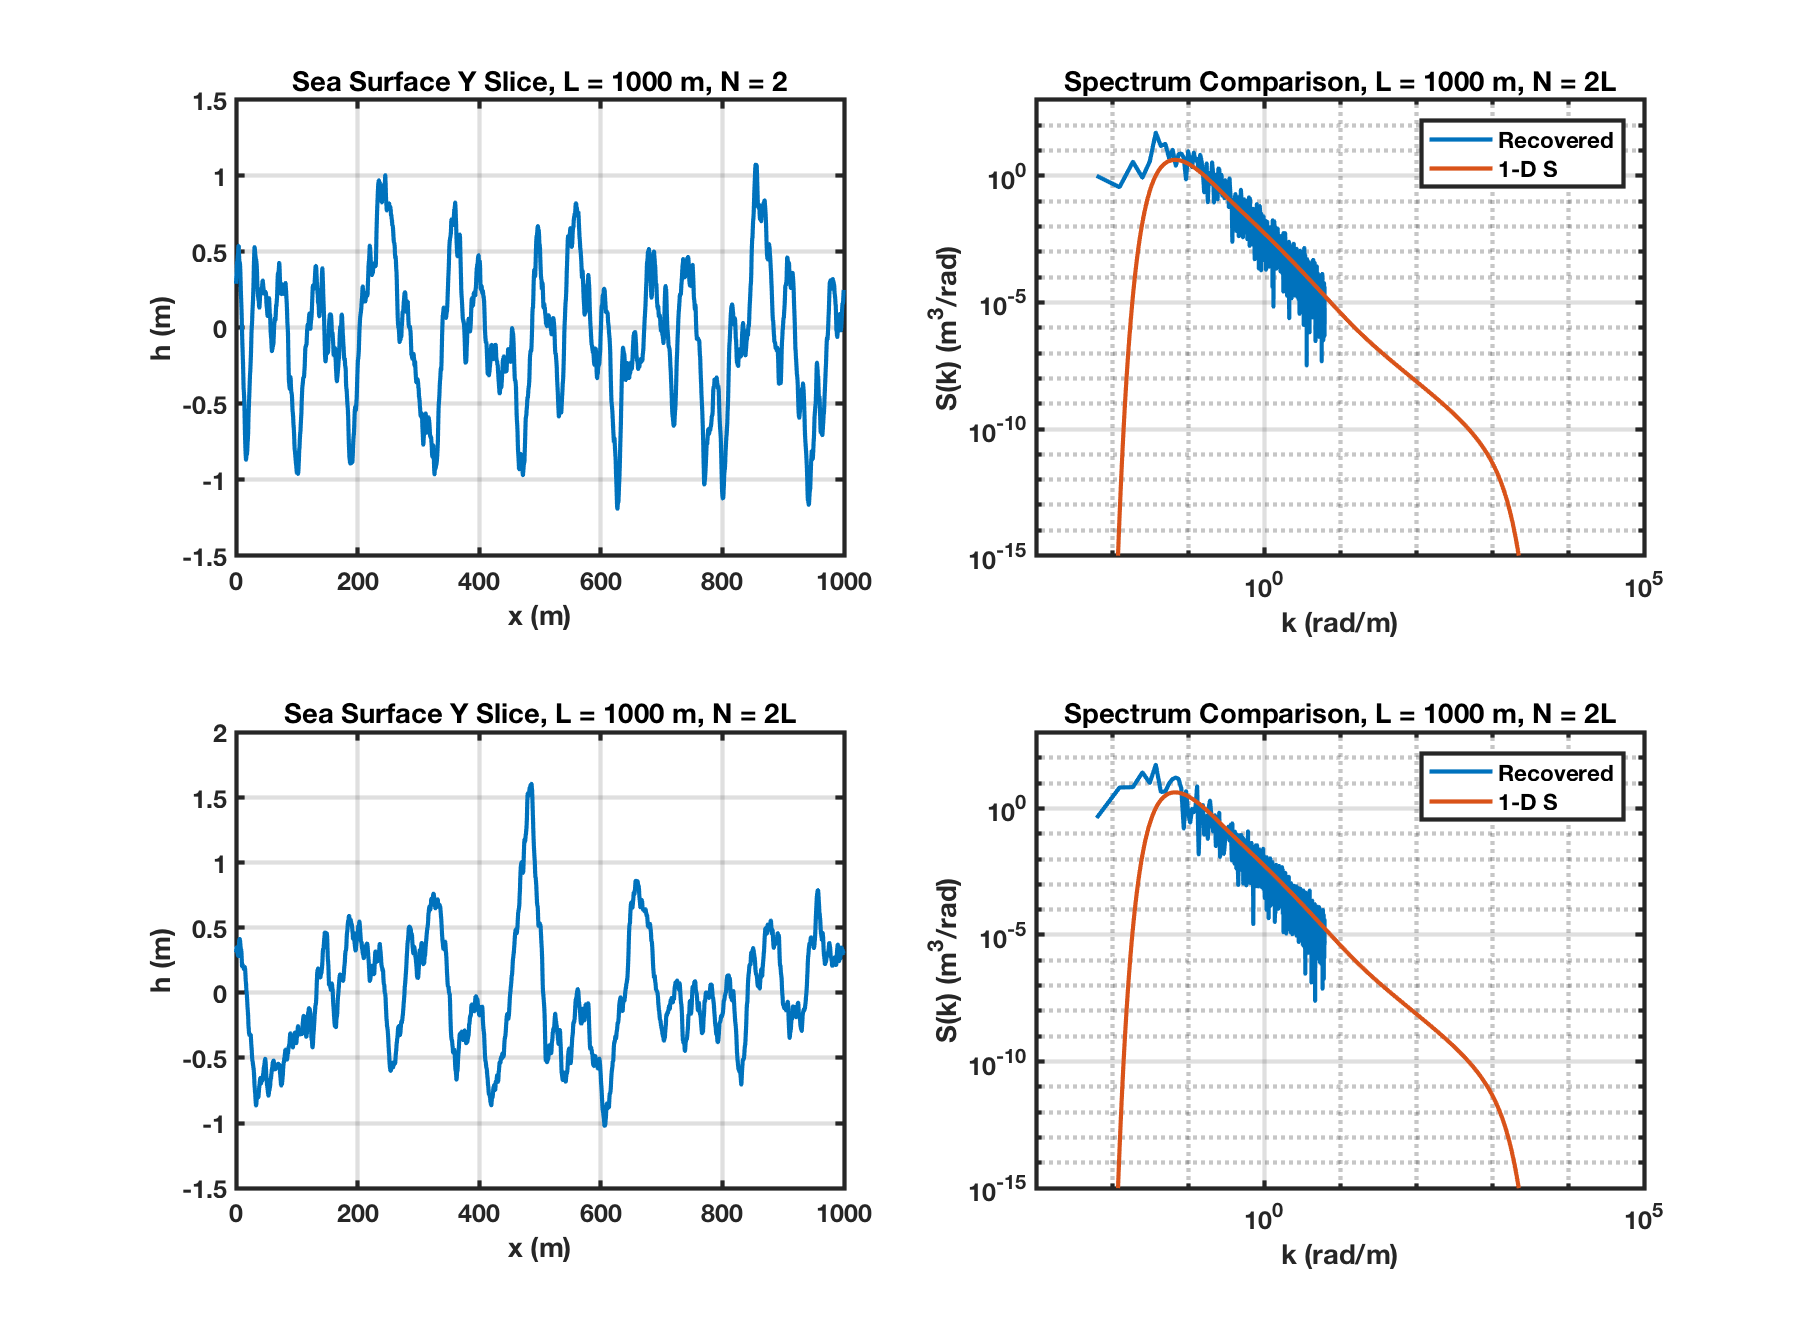
\includegraphics[width=6in]{../media/Ocean_Surface/sea_surface_2d_slices1000.png}
  \end{center}
  \renewcommand{\baselinestretch}{1} \small\normalsize
  \begin{quote}
    \caption[X and Y Slices of 2D Generated Sea Surface]{X and Y Slices of 2D Generated Sea Surface\label{os_fig:10}}
  \end{quote}
\end{figure}
\renewcommand{\baselinestretch}{2} \small\normalsize

\renewcommand{\thechapter}{3}
\chapter{Geometry and Refractivity}

\renewcommand{\thechapter}{4}
\chapter{Numerical Propagation}

\renewcommand{\thechapter}{5}
\chapter{Amplitude Statistics}


\titleformat{\chapter}
      {\normalfont\large}{Appendix \thechapter:}{1em}{}
\newpage
\appendix
\renewcommand{\thechapter}{A}
\renewcommand{\chaptername}{Appendix}
\section{Introduction}
This section provides some background on Green’s functions, presents the convention used in this document for a forward propagating wave, discusses how this convention defines the Fourier transform, and introduces the different types of geometric spreading that may be encountered in propagation.

\subsection{Background}
In 1828, an English mathematician named George Green published "An Essay on the Application of Mathematical Analysis to the Theories of Electricity and Magnetism" with a theorem that is now used extensively to solve differential equations in electromagnetics, quantum mechanics, and applied mathematics \cite{green_phys_today}. Unfortunately, the scope of his contributions weren’t realized until after his death. 

Today, Green's functions are a useful tool in solving inhomogeneous differential equations and can be thought of as the impulse response for the differential equation. There are many references for Green's functions from the mathematical perspective \cite{bender_orszag}, \cite{arfken_weber}, \cite{gbur_math}, \cite{guenther_partial_de}, \cite{duffy_green}, and for their application to electromagnetics \cite{jackson_classical_em}, \cite{zangwill_modern_em}, \cite{balanis_advanced}, \cite{goodman_fourier}, \cite{smith_radiation}. Unfortunately, these references typically only highlight one aspect and have conflicting conventions for propagation direction and normalization. In addition, they tend to skip over many steps, and some define Green's functions without really using them, while others use Green’s Functions without really defining them. The purpose of this document is to work through derivations of the canonical free space Green's functions and demonstrate in a consistent manner how they can be utilized in electromagnetic propagation problems where diffraction becomes important. A particular aspect covered here is the derivation of equations governing the propagation of Radio Frequency (RF) waves in a maritime environment.

\subsection{Time Dependence Sign Convention} \label{gf_sec:time_dependence}
Before getting started, we need to define the sign convention used for time dependence. We  assume harmonic propagating waves that follow the typical Engineering literature with time dependence going as $e^{j\omega t}$. This means we can represent an arbitrary vector wave $\mathbf{C}(\mathbf{r},t)$ as:

\begin{equation}
\mathbf{C}\left(\mathbf{r},t\right) = \mathbf{C}\left(\mathbf{r}\right)e^{j\omega t}
\label{gf_eq:0a}
\end{equation}
\renewcommand{\baselinestretch}{2} \small\normalsize

For a system to be causal, it may only depend on past or present inputs and not on future inputs. Any physically realizable system, such as an electromagnetic wave must be causal, as something that has not yet happened cannot have an impact on the current output. We can relate the causality condition to the phase with the restriction that the phase can be delayed but not advanced. This tells us that for propagating waves, we need to look for solutions in the form of $g\left(\pm\left[\omega t - k_or\right]\right)$, as solutions in the form of $g\left(\pm\left[\omega t + k_or\right]\right)$ advance the phase and are not physically realizable. 

With this restriction, our vector waves from Equation \ref{gf_eq:0a} must take the form:

\begin{equation}
\mathbf{C}\left(\mathbf{r},t\right) = \mathbf{C}e^{j\left(\omega t - \mathbf{k}_o \cdot \mathbf{r} \right)}
\label{gf_eq:18b}
\end{equation}
\renewcommand{\baselinestretch}{2} \small\normalsize

In the next section, we will see that this choice of time dependence  defines the forward and reverse Fourier transforms in both the temporal and spatial domains.

\subsection {Fourier Transforms in Time and Space} \label{gf_sec:fourier_transform}
We must remain self consistent with our sign conventions when using Fourier transforms. The easiest way to ensure consistency is to interpret the transform from a frequency domain to either the temporal or spatial domain as a superposition of the signal of interest with forward propagating waves over all frequencies. The sign convention for the Fourier transform then comes directly from our definition of a forward propagating wave from the previous section.  

Table \ref{gf_tab:0a} presents the forward Fourier transforms, $\hat{g} = \mathcal{F}\{g\}$, and the inverser Fourier transforms, $g = \mathcal{F}^{-1}\{\hat{g}\}$, in both time and space for an arbitrary function, $g$, and its Fourier transform, $\hat{g}$.
\begin{table}[ht]
  \begin{center}
      \renewcommand{\baselinestretch}{1} \small\normalsize
  \begin{quote}
    \caption[Fourier Transforms in Time and Space]{Fourier Transforms in Time and Space\label{gf_tab:0a}}
  \end{quote}
  \begin{tabular} {|c | c | c|}
    \hline
  \bf{Domain} & \bf{Forward Transform} & \bf{Inverse Transform}\\ \hline
  Time & $\displaystyle \hat{g}(\omega) = \int_{-\infty}^{\infty} g(t)e^{-j\omega t}dt$ & $\displaystyle  g(t) = \frac{1}{2\pi}\int_{-\infty}^\infty \hat{g}(\omega)e^{j\omega t}d\omega$\\ \hline
 Space & $\displaystyle \hat{g}(k) = \int_{-\infty}^{\infty} g(x)e^{jk x}dx$ & $\displaystyle  g(x) = \frac{1}{2\pi}\int_{-\infty}^\infty \hat{g}(k)e^{-jk x}dk$\\ \hline
\end{tabular}
\end{center}
\end{table}
\renewcommand{\baselinestretch}{2} \small\normalsize

\subsection{Geometric Spreading}
The geometric spreading of an electromagnetic wave is dependent on the dimensionality and approximations used. A plane wave is easy to work with but shows no spreading or amplitude reduction as it propagates. A paraxial wave allows us to represent beam like waves and will have spreading proportional to $1/\sqrt{L_x}$, where $L_x$ is the length along the propagation direction. A cylindrical wave will have spreading proportional to $1/\sqrt{\rho}$ and a spherical wave will have spreading proportional to $1/r$. The amount of geometry induced spreading increases as we add higher fidelity to our models and analytical tools so we need to take that into consideration when comparing models.

\section {Green's Identities and Method}
The two identities named for George Green and the method of Green’s functions will be derived in this section.

\subsection{Identities}
To derive Green’s identities, we will start with the divergence theorem:

\begin{equation}
\oint\limits_{S} \mathbf{C} \cdot \hat{n} dS = \int\limits_{V}d^3r'\nabla \cdot \mathbf{C}
\label{gf_eq:1}
\end{equation}
\renewcommand{\baselinestretch}{2} \small\normalsize

By replacing the vector $\mathbf{C}$ with a function of two arbitrary scalar variables, $\mathbf{C}=\varphi\nabla\psi$, we get:

\begin{equation}
\oint\limits_{S} \varphi\nabla\psi \cdot \hat{n} dS = \int\limits_{V}d^3r'\nabla \cdot \varphi\nabla\psi
\label{gf_eq:2}
\end{equation}
\renewcommand{\baselinestretch}{2} \small\normalsize

Using the identity $\nabla\psi\cdot \hat{n} = \partial \psi/\partial n$ and expanding the dot product in the volume integral yields Green's first identity:

\begin{equation}
\boxed{\oint\limits_{S} \varphi\frac{\partial \psi}{\partial n} dS = \int\limits_{V}d^3r' \left[ \nabla\varphi \cdot \nabla\psi +\varphi \nabla^2 \psi\right]}
\label{gf_eq:3}
\end{equation}
\renewcommand{\baselinestretch}{2} \small\normalsize

If we flip the order of the scalar variables and instead let $\mathbf{C}=\psi\nabla\varphi$, Green's first identity is expressed as:

\begin{equation}
\oint\limits_{S} \psi\frac{\partial \varphi}{\partial n} dS = \int\limits_{V}d^3r' \left[ \nabla\psi \cdot \nabla\varphi +\psi \nabla^2 \varphi\right]
\label{gf_eq:4}
\end{equation}
\renewcommand{\baselinestretch}{2} \small\normalsize

\noindent Subtracting Equation \ref{gf_eq:4} from Equation \ref{gf_eq:3} yields Green's second identity:

\begin{equation}
\boxed{\oint\limits_{S} \left[ \varphi\frac{\partial \psi}{\partial n} - \psi\frac{\partial \varphi}{\partial n} \right]dS = \int\limits_{V}d^3r' \left[ \varphi\nabla^2\psi- \psi \nabla^2 \varphi\right]}
\label{gf_eq:5}
\end{equation}

\subsection {Method of Green's Functions} \label{gf_sec:method}
For the purposes of this document, we are interested in time varying propagation problems. Therefore, we would like to apply the method of Green's functions to the scalar wave equation  to solve for the scalar field $\varphi$ as a function of space and time with an arbitrary driving function, $f$, that is also a function of space and time:

\begin{equation}
\nabla^2\varphi\left(\mathbf{r},t\right) - \frac{1}{c^2}\frac{\partial^2 \varphi\left(\mathbf{r},t\right)}{\partial t^2} = f\left(\mathbf{r},t\right)
\label{gf_eq:6}
\end{equation}
\renewcommand{\baselinestretch}{2} \small\normalsize

\noindent We can utilize the Fourier transform to remove the time dependence:

\begin{equation}
\nabla^2\varphi\left(\mathbf{r},\omega\right) + \frac{\omega^2}{c^2}\varphi\left(\mathbf{r},\omega\right) = f\left(\mathbf{r},\omega\right)
\label{gf_eq:7}
\end{equation}
\renewcommand{\baselinestretch}{2} \small\normalsize

Equation \ref{gf_eq:7} is the Helmholtz equation and it represents the wave equation with only spatial derivatives. If we use the wavevector, $k_o = \omega/c$, and suppress the variable dependence for clarity, Equation \ref{gf_eq:7} can be rewritten as:

\begin{equation}
\nabla^2\varphi + k_o^2\varphi = f
\label{gf_eq:8}
\end{equation}
\renewcommand{\baselinestretch}{2} \small\normalsize

The Green's function for this problem can be found by replacing the driving function, $f$, with a delta function:

\begin{equation}
\nabla^2G+ k_o^2G = -\delta\left(\mathbf{r}-\mathbf{r}' \right)
\label{gf_eq:9}
\end{equation}
\renewcommand{\baselinestretch}{2} \small\normalsize

Equation \ref{gf_eq:9} shows that the Green's function is the solution to the differential equation for a spatial impulse and therefore represents the impulse response of the system. In electromagnetics, the driving force often has a negative sign as seen from the Laplace equation, $\nabla^2\varphi = -\rho/\epsilon_o$, so we typically chose a matching negative sign for the delta function. With this convention, we need to make sure the driving force has a negative sign when utilizing a Green's function later.

The general method to find Green's functions is to solve the homogeneous differential equation away from the delta function source and then integrate over a small region that includes the delta function for normalization. Some authors, such as \cite{jackson_classical_em}, include a $4\pi$ scale factor with the delta function to absorb this normalization term into the differential equation rather than the Green's function.

Equations \ref{gf_eq:8} and \ref{gf_eq:9} can be rearranged to solve for the Laplacian, so that $\nabla^2\varphi = f - k_o^2\varphi$ and $\nabla^2G = -\delta\left(\mathbf{r}-\mathbf{r}' \right) - k_o^2G$. We can substitute these values into Green's second identity (Equation \ref{gf_eq:5}), with $\psi=G$:

\begin{equation}
\begin{gathered}
\oint\limits_{S} \left[ \varphi\frac{\partial G}{\partial n} - G\frac{\partial \varphi}{\partial n} \right]dS = \int\limits_{V}d^3r' \left[ \varphi\nabla^2G- G \nabla^2 \varphi\right] \\
\oint\limits_{S} \left[ \varphi\frac{\partial G}{\partial n} - G\frac{\partial \varphi}{\partial n} \right]dS = \int\limits_{V}d^3r' \left[ \varphi \left(-\delta\left(\mathbf{r}-\mathbf{r}' \right) - k_o^2G\right)- G \left(f - k_o^2\varphi \right)\right] \\
\int\limits_{V}d^3r'\varphi\delta\left(\mathbf{r}-\mathbf{r}' \right) = \oint\limits_{S}\left[G\frac{\partial \varphi}{\partial n} - \varphi\frac{\partial G}{\partial n} \right]dS +\int\limits_{V}d^3r'\left[ Gk_o^2\varphi - \varphi k_o^2G-k_o^2G - Gf \right] \\
\int\limits_{V}d^3r'\varphi\delta\left(\mathbf{r}-\mathbf{r}' \right) = \oint\limits_{S}\left[G\frac{\partial \varphi}{\partial n} - \varphi\frac{\partial G}{\partial n} \right]dS -\int\limits_{V}d^3r' Gf
\end{gathered}
\label{gf_eq:10}
\end{equation}
\renewcommand{\baselinestretch}{2} \small\normalsize

As long as $\mathbf{r}'$ is in the volume $V$, we can use the sifting property of the delta function to provide an explicit representation for $\varphi$:

\begin{equation}
\boxed{\varphi = \oint\limits_{S}dS\left[G\frac{\partial \varphi}{\partial n} - \varphi\frac{\partial G}{\partial n} \right] -\int\limits_{V}d^3r' Gf}
\label{gf_eq:11}
\end{equation}
\renewcommand{\baselinestretch}{2} \small\normalsize

Equation \ref{gf_eq:11} defines the general solution for an inhomogeneous differential equation and the only assumption made here is that the forcing function will have a negative sign. The homogeneous solution is given by the surface integral and the response to a forcing function is given by the volume integral. When there are no boundary conditions (as in free space propagation), the normal derivatives are all zero so the surface integral vanishes and we are left with only the term due to the forcing function.

\begin{equation}
\varphi = -\int\limits_{V}d^3r' Gf
\label{gf_eq:11aa}
\end{equation}
\renewcommand{\baselinestretch}{2} \small\normalsize

In the simplest case, $f$ is a delta function with a scalar amplitude, $ f = -\alpha\delta(r'-r_o)$, so that

\begin{equation}
\varphi = \alpha G(r,r_o)
\label{gf_eq:11ab}
\end{equation}
\renewcommand{\baselinestretch}{2} \small\normalsize

\section {Boundary Conditions}
There are two traditional types of boundary conditions: Dirichlet, where $\varphi$ is specified on the boundary, or Neuman, where the normal derivative of $\varphi$ is specified on the boundary. There is a third type of boundary condition, known as the Robin condition, that is a weighted combination of Dirichlet and Neuman boundary conditions.

\subsection {Dirichlet Boundary Conditions}
For Dirichlet boundary conditions, the solution is specified on the surface, $\varphi\left(\mathbf{r}\right) |_{S} = \varphi\left(\mathbf{r}_S \right) = a\left(\mathbf{r}_s\right)$. To simplify Equation \ref{gf_eq:11}, we can enforce the following condition on the Green's function:

\begin{equation}
G\left(\mathbf{r},\mathbf{r}' \right)\bigg|_{S}=0
\label{gf_eq:12}
\end{equation}
\renewcommand{\baselinestretch}{2} \small\normalsize

Green's functions specified in this manner are sometimes called Green's functions of the first kind. Substituting Equation \ref{gf_eq:12} into Equation \ref{gf_eq:11} results in the following equation for $\varphi$ in the presence of Dirichlet boundary conditions.
\begin{equation}
\boxed{\varphi = -\oint\limits_{S}dS \varphi\frac{\partial G}{\partial n} -\int\limits_{V}d^3r' Gf}
\label{gf_eq:13}
\end{equation}
\renewcommand{\baselinestretch}{2} \small\normalsize

\subsection {Neuman Boundary Conditions}
For Neuman boundary conditions, the normal derivative of the field is specified on the surface, $\frac{\partial\varphi\left(\mathbf{r}\right)}{\partial n}|_{S} = b\left(\mathbf{r}_s\right)$. As described in \cite{jackson_classical_em}, \cite{zangwill_modern_em}, and \cite{balanis_advanced}, we cannot simply set the normal derivative of $G$ to $0$. This can be demonstrated by integrating Equation \ref{gf_eq:9} over a volume and then applying the divergence theorem:

\begin{equation}
\begin{gathered}
\int\limits_{V}d^3r' \nabla^2 G = \int\limits_{V}d^3r'\left[-\delta\left(\mathbf{r}-\mathbf{r}' \right) -k^2G \right] \\
\int\limits_{V}d^3r' \nabla \cdot \nabla G = -\int\limits_{V}d^3r'\delta\left(\mathbf{r}-\mathbf{r}' \right) -\int\limits_{V}d^3r'k^2G \\
\oint\limits_{S}\nabla G \cdot \hat{n} dS  = -1 - \int\limits_{V}d^3r'k^2G\\
\oint\limits_{S}\frac{\partial G}{\partial n} dS = -1 - \int\limits_{V}d^3r' k^2G
\end{gathered}
\label{gf_eq:14}
\end{equation}
\renewcommand{\baselinestretch}{2} \small\normalsize

Equation \ref{gf_eq:14} must hold for all values of $k$, so we can find a general condition for $\partial G/\partial n$ by letting $k = 0$:

\begin{equation}
\oint\limits_{S}\frac{\partial G}{\partial n} dS = -1
\label{gf_eq:15}
\end{equation}
\renewcommand{\baselinestretch}{2} \small\normalsize

Equation \ref{gf_eq:15} indicates that there is a discontinuity in the normal derivative of the Green's function. Letting $S$ be the total surface area gives us the following condition on the normal derivative of the Green's function:

\begin{equation}
\frac{\partial G}{\partial n} = -\frac{1}{S}
\label{gf_eq:16}
\end{equation}
\renewcommand{\baselinestretch}{2} \small\normalsize

Equation \ref{gf_eq:16} demonstrates the jump condition for the normal derivative of the Green's function. Note that when the surface is taken out to infinity that $\partial G/\partial n = 0$. Green's functions specified in this manner are sometimes called Green's functions of the second kind. Substituting Equation \ref{gf_eq:16} into Equation \ref{gf_eq:11} results in the following equation for $\varphi$ in the presence of Neuman boundary conditions.

\begin{equation}
\boxed{\varphi = \oint\limits_{S}dS\left[G\frac{\partial \varphi}{\partial n} + \frac{\varphi}{S} \right] -\int\limits_{V}d^3r' Gf}
\label{gf_eq:17}
\end{equation}
\renewcommand{\baselinestretch}{2} \small\normalsize

We can rewrite Equation \ref{gf_eq:17} as in \cite{jackson_classical_em}, using the average value of the solution over the surface, $\left< \varphi\right> = \frac{1}{S}\oint\limits_{S}\varphi dS$:

\begin{equation}
\boxed{\varphi = \left<\varphi \right> + \oint\limits_{S}G\frac{\partial \varphi}{\partial n}dS  -\int\limits_{V}d^3r' Gf}
\label{gf_eq:18}
\end{equation}
\renewcommand{\baselinestretch}{2} \small\normalsize

\subsection {Robin Boundary Conditions}
For Robin boundary conditions, a weighted linear combination of the solution and its derivative are specified on the surface, $\frac{\partial\varphi\left(\mathbf{r}\right)}{\partial n}|_{S} +\alpha\varphi\left(\mathbf{r}\right) |_{S}= c\left(\mathbf{r}_s\right)$. 

We can generally set $c=0$ so that the Robin boundary condition relates the Green's function on the surface to its normal derivative on the surface.

\begin{equation}
\frac{\partial G\left(\mathbf{r}\right)}{\partial n}\bigg|_{S} = -\alpha G
\label{gf_eq:18aa}
\end{equation}
\renewcommand{\baselinestretch}{2} \small\normalsize

Substituting Equation \ref{gf_eq:18aa} into Equation \ref{gf_eq:11} results in the following equation for $\varphi$ in the presence of Robin boundary conditions.

\begin{equation}
\boxed{\varphi = \oint\limits_{S}dS\left[\frac{\partial \varphi}{\partial n} + \alpha\varphi \right] -\int\limits_{V}d^3r' Gf}
\label{gf_eq:18aabb}
\end{equation}
\renewcommand{\baselinestretch}{2} \small\normalsize

Robin boundary conditions are commonly found in propagation problems with mixed polarization. They generally do not allow simple solutions are usually solved numerically.

\section {Properties of Green's Functions} \label{gf_sec:properties}
We have already discussed the fact that Green's functions represent the spatial impulse response of the differential equation. This section introduces some other properties of Green's functions, including causality, reciprocity, continuity, and general forms.

\subsection {Causality} \label{gf_sec:causality}
Green’s functions represent physical systems and therefore must be causal. With the time dependence as specified in Section \ref{gf_sec:time_dependence}, our solutions must have the following form:

\begin{equation}
G\left(r,t\right) \sim g\left(\omega t - k_or\right)
\label{gf_eq:18a}
\end{equation}
\renewcommand{\baselinestretch}{2} \small\normalsize

\subsection {Reciprocity} \label{gf_sec:reciprocity}
Green's functions must be symmetric with respect to $\mathbf{r}$ (the vector to the observer) and $\mathbf{r}'$ (the vector to the source), so that:

\begin{equation}
G\left(\mathbf{r},\mathbf{r}' \right) = G\left(\mathbf{r}',\mathbf{r} \right)
\label{gf_eq:18c}
\end{equation}
\renewcommand{\baselinestretch}{2} \small\normalsize

This property is known as reciprocity and it tells us that the impulse reponse for a propagating wave is the same in both directions. Reciprocity is commonly used in antenna radiation analysis as it allows us to analyze an antenna considering it as either a transmitter or a receiver.

\subsection {Continuity} \label{gf_sec:continuity}
A necessary condition for reciprocity is that Green's functions must be continuous in all space. However, they are singular so the derivative will have a discontinuity at $\mathbf{r} = \mathbf{r}'$.

\subsection {General Forms}
Because a Green's function is the spatial impulse response of the system, we can expect it to be used in a convolution integral. With that in mind, Green's functions usually take the form:
\begin{equation}
G\left(\mathbf{r},\mathbf{r}' \right) = g\left( \mathbf{r} - \mathbf{r}'\right)
\label{gf_eq:18d}
\end{equation}
\renewcommand{\baselinestretch}{2} \small\normalsize

Using the results of the previously described properties, the most general representation of a Green's function is as follows:

\begin{equation}
G\left(\mathbf{r},\mathbf{r}',t ,t'\right) = g\left(\omega |t-t'| - k| \mathbf{r} - \mathbf{r}' | \right)
\label{gf_eq:19b}
\end{equation}
\renewcommand{\baselinestretch}{2} \small\normalsize

\section {Free Space Green's Functions}
This section derives the free space Green's functions for the Helmholtz equation (Equation \ref{gf_eq:9}) in both 3-dimensions and 2-dimensions. In the 2-dimensional case, we will also derive the Green's function for the paraxial wave equation. In free space, there are no boundaries, so we can let $r\rightarrow \infty$ and use Dirichlet boundary conditions at $\infty$. Without loss of generality, we can place the delta function at the origin, so that $\delta\left(\mathbf{r}-\mathbf{r}' \right) \rightarrow \delta \left(\mathbf{r} \right)$. To find the Green's function, we need to solve the homogeneous equation away from the delta function and then integrate over a small region around the origin for normalization. The homogenous equation to solve is:

\begin{equation}
\nabla^2G+ k_o^2G = 0
\label{gf_eq:19}
\end{equation}
\renewcommand{\baselinestretch}{2} \small\normalsize

Because the delta function is rotationally symmetric, the Green's function must also be rotationally symmetric.

\subsection {3-Dimensions}\label{gf_sec:3d}
This section derives the free space Green's function for the Helmholtz equation in 3-dimensional space. Because we used the Fourier transform to remove the time dependence from the wave equation (Equation 
\ref{gf_eq:6}), we will first work in the frequency domain and then transform the result back to the time domain.

\subsubsection {Deriviation in the Frequency Domain}
In 3-dimensions,  rotational symmetry means that  $\partial G/\partial\theta = \partial G/\partial\phi=0$. Therefore we can expand the Laplacian of Equation \ref{gf_eq:19} in spherical coordinates and neglect the $\theta$ and $\phi$ components:

\begin{equation}
\frac{1}{r^2}\frac{\partial}{\partial r}\left(r^2\frac{\partial G}{\partial r}\right)+ k_o^2G = 0
\label{gf_eq:20}
\end{equation}
\renewcommand{\baselinestretch}{2} \small\normalsize

Expanding the derivatives in Equation \ref{gf_eq:20} along with a little algebraic manipulation allows us to rewrite this into something more manageable:

\begin{equation}
\begin{gathered}
\frac{1}{r^2}\left[2r\frac{\partial G}{\partial r}+ r^2\frac{\partial^2 G}{\partial r^2}  \right] + k_o^2G = 0 \\
r\frac{\partial^2 G}{\partial r^2} + 2\frac{\partial G}{\partial r}+ k_o^2rG = 0 \\
\frac{\partial^2 \left(rG\right)}{\partial r^2} + k_o^2rG = 0
\end{gathered}
\label{gf_eq:21}
\end{equation}
\renewcommand{\baselinestretch}{2} \small\normalsize

Equation \ref{gf_eq:21} has the following  solution:

\begin{equation}
G = c_1\frac{e^{jk_or}}{r} + c_2\frac{e^{-jk_or}}{r}
\label{gf_eq:22}
\end{equation}
\renewcommand{\baselinestretch}{2} \small\normalsize

From the causality restriction discussed in Section \ref{gf_sec:causality}, the $c_2$ term describes an outward propagating wave. This is the physical solution, which means $c_1$ must be equal to $0$. Therefore, the free space Green's function is:

\begin{equation}
G = c_2\frac{e^{-jk_or}}{r}
\label{gf_eq:23}
\end{equation}
\renewcommand{\baselinestretch}{2} \small\normalsize

This equation represents a spherical wave and is valid everywhere except $r=0$. To find $c_2$, we need to integrate Equation \ref{gf_eq:9} over a small volume centered at $r=0$ and then take the limit as $r\rightarrow0$.

\begin{equation}
\begin{gathered}
\lim_{r\to0}\int\limits_{V}d^3r'\left[\nabla^2G+ k_o^2G\right] = -\lim_{r\to0}\int\limits_{V}\delta\left(\mathbf{r}\right) \\
\lim_{r\to0}\int\limits_{V}d^3r'\left[\nabla \cdot\nabla G+ k_o^2G\right] = -1 \\
\lim_{r\to0}\left[\oint\limits_{S}\nabla G \cdot \hat{n} dS + \int\limits_{V}d^3r' k_o^2G\right] = -1 \\
\lim_{r\to0}\left[\oint\limits_{S}\frac{\partial G}{\partial n} dS + \int\limits_{V}d^3r' k_o^2G\right] = -1
\end{gathered}
\label{gf_eq:24}
\end{equation}
\renewcommand{\baselinestretch}{2} \small\normalsize

Substituting Equation \ref{gf_eq:23} in for $G$ and letting $\hat{n} = \hat{r}$, $dS = r'^2\sin{\theta'}d\theta' d\phi'$, and  $d^3r' = r'^2\sin{\theta'}dr'd\theta' d\phi'$ yields:

\begin{equation}
\begin{gathered}
\lim_{r\to0}\left[c_2\oint\limits_{S}\frac{\partial }{\partial r'}\frac{e^{-jk_or'}}{r'} r'^2\sin{\theta'} d\theta' d\phi '+ c_2\int\limits_{V}r'^2 \sin{\theta'}dr' d\theta' d\phi' k_o^2\frac{e^{-jk_or'}}{r'}\right] = -1 \\
\lim_{r\to0}\left[c_2 r^2\left( \frac{jk_o}{r} - \frac{1}{r^2}\right)e^{-jk_or}\oint\limits_{S}\sin{\theta'} d\theta' d\phi' + c_2\int\limits_{V}dr' d\theta' d\phi' k_o^2r'e^{-jk_or'}\sin{\theta'}\right] = -1 \\
\lim_{r\to0}\left[4\pi c_2 \left( jk_or - 1\right)e^{-jk_or}+ 4\pi c_2k_o^2\int\limits_{V}dr' r'e^{-jk_or'}\right] = -1 \\
\lim_{r\to0}4\pi c_2\left[\left( jk_or - 1\right)e^{-jk_or}+ k_o^2\int\limits_{V}dr' \frac{\partial}{\partial k_o}\frac{e^{-jk_or'}}{j}\right] = -1 \\
4\pi c_2\left[-1 +  \lim_{r\to0}\frac{k_o^2}{j}\frac{\partial}{\partial k_o}\left( \frac{-1}{jk_o}e^{-jk_or'}\right)\bigg|_0^{r}  \right] = -1 \\
-4\pi c_2\left[1 - \lim_{r\to0}k_o^2\frac{\partial}{\partial k_o}\left( \frac{1}{k_o}e^{-jk_o} - \frac{1}{k_o}\right) \right] = -1 \\
c_2\left[1 - \lim_{r\to0}k_o^2\left(-\frac{1}{k_o^2}+\frac{-jre^{-jk_or}}{k_o}+\frac{1}{k_o^2}\right) \right] = \frac{1}{4\pi} \\
 c_2 = \frac{1}{4\pi}
\end{gathered}
\label{gf_eq:25}
\end{equation}
\renewcommand{\baselinestretch}{2} \small\normalsize

\noindent Now letting $r \rightarrow |\mathbf{r}-\mathbf{r}'|$, we have the final free space 3-dimensional Green's function, $G_o$:

\begin{equation}
\boxed{G_o\left(\mathbf{r},\mathbf{r}'\right) = \frac{e^{-jk_o|\mathbf{r} - \mathbf{r}'|}}{4\pi |\mathbf{r} - \mathbf{r}'|}}
\label{gf_eq:26}
\end{equation}
\renewcommand{\baselinestretch}{2} \small\normalsize

As discussed for Equation \ref{gf_eq:9}, some authors, such as \cite{jackson_classical_em}, include the $4\pi$ scale factor with the delta function, so the free space 3-dimensional Green's function is:

\begin{equation}
G_o\left(\mathbf{r},\mathbf{r}'\right)  = \frac{e^{-jk_o|\mathbf{r} - \mathbf{r}'|}}{|\mathbf{r} - \mathbf{r}'|}
\label{gf_eq:27}
\end{equation}
\renewcommand{\baselinestretch}{2} \small\normalsize

\noindent In this case, the $4\pi$ scale factor would then appear in Equation \ref{gf_eq:11}.

To help visualize this Green's function, the magnitude and phase is shown in Figure \ref{gf_fig:1} and the real and imaginary components are shown in Figure \ref{gf_fig:2}. These figures constrain the Green's function to the $x-y$ plane at $z=0$ for visualization.

\begin{figure}[ht]
\begin{center}
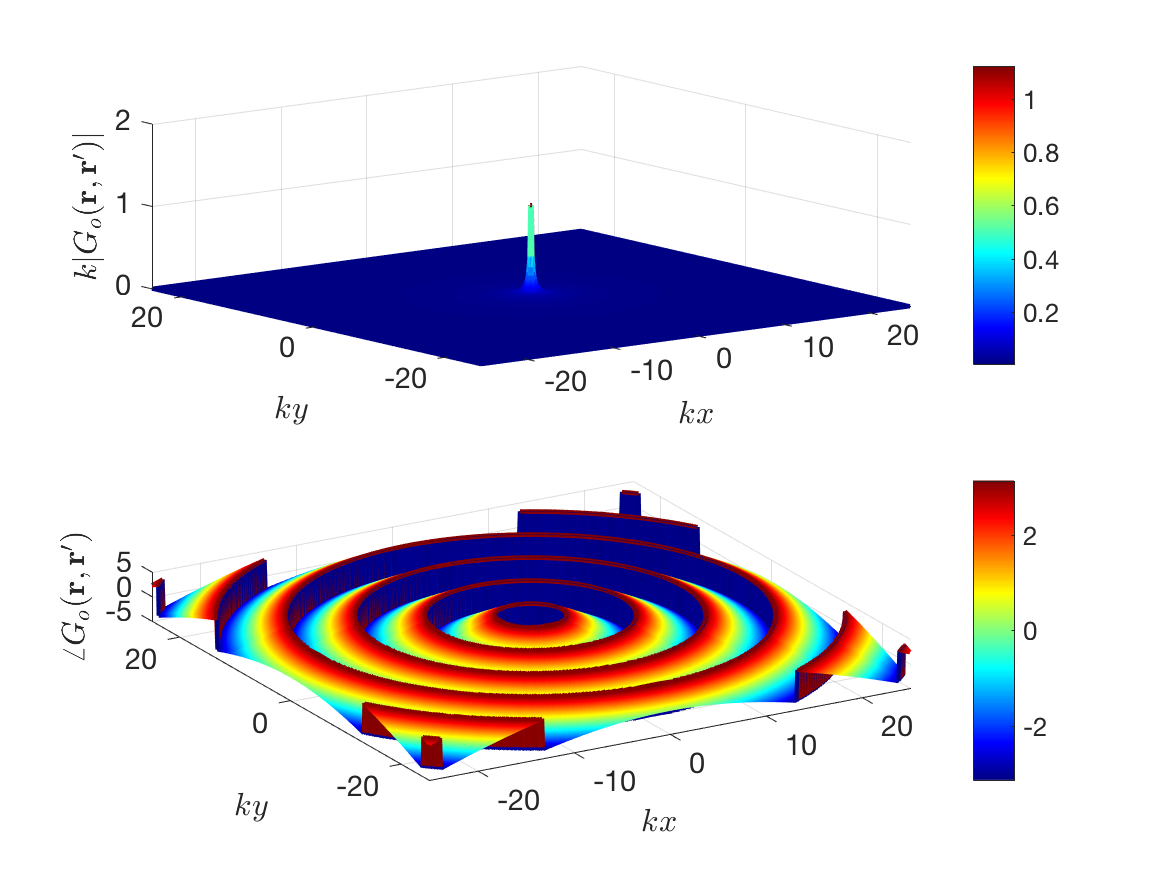
\includegraphics[width=4in]{../media/3d_fs_gf_mag.png}
\end{center}
\renewcommand{\baselinestretch}{1}
\small\normalsize
\begin{quote}
\caption[Magnitude and Phase of 3-D Free Space Green's Function]{ Magnitude and Phase of 3-D Free Space Green's Function\label{gf_fig:1}}
\end{quote}
\end{figure} 
\renewcommand{\baselinestretch}{2}
\small\normalsize

\begin{figure}[ht]
\begin{center}
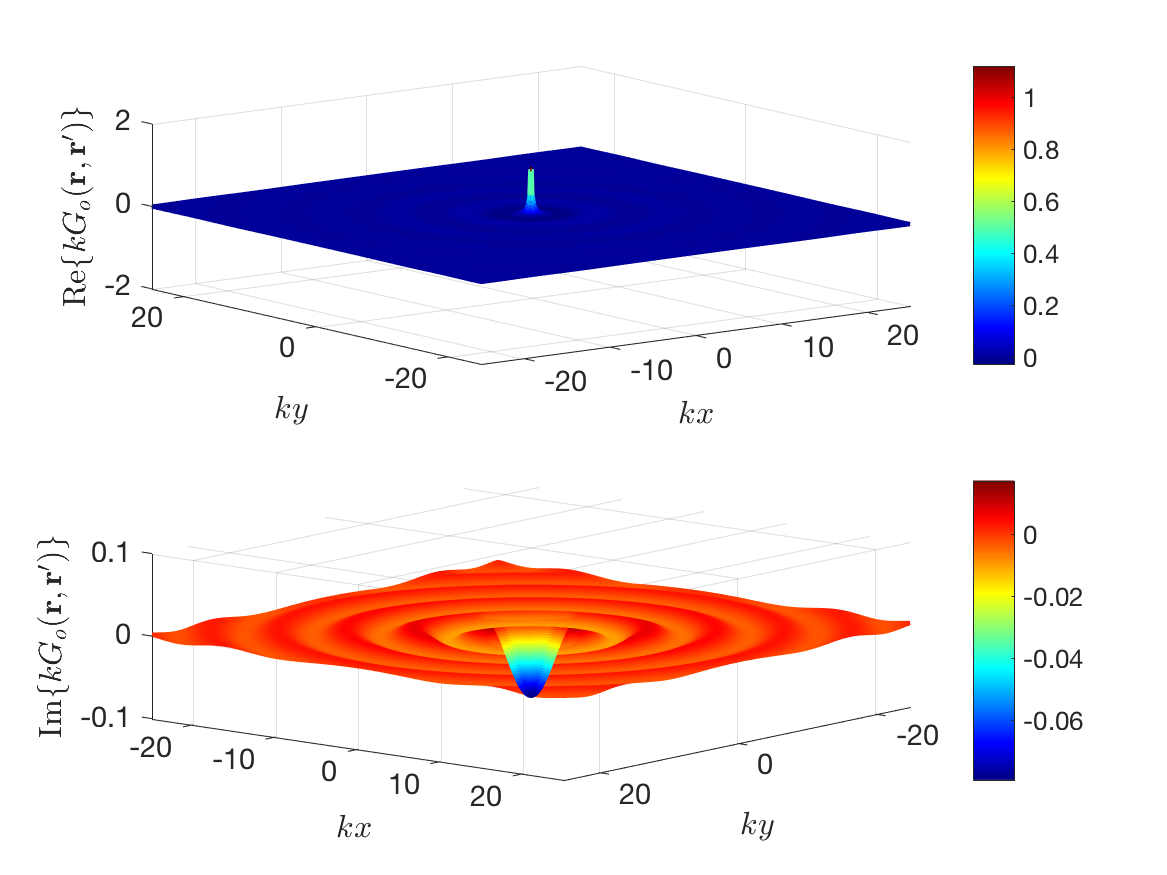
\includegraphics[width=4in]{../media/3d_fs_gf_re_im.png}
\end{center}
\renewcommand{\baselinestretch}{1}
\small\normalsize
\begin{quote}
\caption[Real and Imaginary Components of 3-D Free Space Green's Function]{Real and Imaginary Components of 3-D Free Space Green's Function \label{gf_fig:2}}
\end{quote}
\end{figure} 
\renewcommand{\baselinestretch}{2}
\small\normalsize

\subsubsection {Conversion to the Time Domain}
The Green's function in Equation \ref{gf_eq:26} is still in Fourier space. We can explicitly express the frequency dependence as:

\begin{equation}
G_o\left(\mathbf{r},\mathbf{r}',\omega\right) = \frac{e^{-j\frac{\omega}{c}|\mathbf{r} - \mathbf{r}'|}}{4\pi |\mathbf{r} - \mathbf{r}'|}
\label{gf_eq:28}
\end{equation}
\renewcommand{\baselinestretch}{2} \small\normalsize

\noindent To determine the Green's function in the time domain, we need to take the inverse Fourier transform.

\begin{equation}
\begin{gathered}
G_o\left(\mathbf{r},\mathbf{r}',t\right) = \frac{1}{2\pi}\int\limits_{-\infty}^{\infty}d\omega e^{j\omega t}G_o\left(\mathbf{r},\mathbf{r}',\omega\right) \\
G_o\left(\mathbf{r},\mathbf{r}',t\right) = \frac{1}{2\pi}\int\limits_{-\infty}^{\infty}d\omega e^{j\omega t}  \frac{e^{-j\frac{\omega}{c}|\mathbf{r}-\mathbf{r}'|}}{4\pi |\mathbf{r}-\mathbf{r}'|}\\
G_o\left(\mathbf{r},\mathbf{r}',t\right) = \frac{1}{4\pi |\mathbf{r}-\mathbf{r}'|}\frac{1}{2\pi}\int\limits_{-\infty}^{\infty}d\omega e^{-j\omega\left(\frac{|\mathbf{r}-\mathbf{r}'|}{c} - t\right)} \\
G_o\left(\mathbf{r},\mathbf{r}',t\right) = \frac{1}{4\pi |\mathbf{r}-\mathbf{r}'|}\frac{1}{2\pi}\int\limits_{-\infty}^{\infty}d\omega e^{-j\omega\left(t - \frac{|\mathbf{r}-\mathbf{r}'|}{c}\right)}
\end{gathered}
\label{gf_eq:29}
\end{equation}
\renewcommand{\baselinestretch}{2} \small\normalsize

\noindent Recognizing that the Fourier transform of the delta function is:

\begin{equation}
\delta(t-t_0) = \frac{1}{2\pi}\int\limits_{-\infty}^{\infty}d\omega e^{-j\omega \left(t-t_0\right)}
\label{gf_eq:30}
\end{equation}
\renewcommand{\baselinestretch}{2} \small\normalsize

\noindent We can write the free space Green's function in the temporal domain as:

\begin{equation}
\boxed{G_o\left(\mathbf{r},\mathbf{r}',t\right) = \frac{\delta\left(t-\frac{|\mathbf{r}-\mathbf{r}'|}{c} \right)}{4\pi |\mathbf{r}-\mathbf{r}'|}}
\label{gf_eq:31}
\end{equation}
\renewcommand{\baselinestretch}{2} \small\normalsize

Equation \ref{gf_eq:31} assumes the source is turned on at time $0$. If we let the source be turned on at an arbitrary time, $t'$, a more general expression is:

\begin{equation}
G_o\left(\mathbf{r},\mathbf{r}',t,t'\right) = \frac{\delta\left(|t-t'|-\frac{|\mathbf{r}-\mathbf{r}'|}{c} \right)}{4\pi |\mathbf{r}-\mathbf{r}'|}
\label{gf_eq:32}
\end{equation}
\renewcommand{\baselinestretch}{2} \small\normalsize

In the time domain, we generally refer to $G_o\left(\mathbf{r},\mathbf{r}',t, t'\right)$ as the retarded wave solution because an observer will experience the source as if it acted at an earlier (retarded) time, $t_1=|t-t'|-|\mathbf{r}-\mathbf{r}'|/c$.

\subsection {2-Dimensions}\label{gf_sec:2d}
This section derives the free space Green's function for the Helmholtz equation in 2-dimensional space. We will again work in the frequency domain first and then transform the result back to the time domain.

\subsubsection {Deriviation in the Frequency Domain}
In 2-dimensions,  rotational symmetry means that  $\partial G/\partial\phi =0$. Therefore we can expand the Laplacian of Equation \ref{gf_eq:19} in polar coordinates and neglect the $\phi$ components:

\begin{equation}
\frac{1}{\rho}\frac{\partial}{\partial \rho}\left(\rho\frac{\partial G}{\partial \rho}\right)+ k_o^2G = 0
\label{gf_eq:33}
\end{equation}
\renewcommand{\baselinestretch}{2} \small\normalsize

\noindent Equation \ref{gf_eq:33} is Bessel's equation with $\nu = 0$:

\begin{equation}
\frac{1}{\rho}\frac{\partial}{\partial \rho}\left(\rho\frac{\partial G}{\partial \rho}\right)+ \left(k_o^2 -\nu^2\right)G = 0
\label{gf_eq:34}
\end{equation}
\renewcommand{\baselinestretch}{2} \small\normalsize

\noindent The general solution to Equation \ref{gf_eq:33} is 

\begin{equation}
G = c_1J_0\left(k_o\rho\right) + c_2N_0\left(k_o\rho\right)
\label{gf_eq:35}
\end{equation}
\renewcommand{\baselinestretch}{2} \small\normalsize

Here $J_0$ is a Bessel function of the first kind, and $N_0$ is a Bessel function of the second kind. Since the delta function is singular at the origin, we cannot demand that $G$ be finite at the origin. This means that $c_2 \neq 0$ and we have one equation with two unknowns.

When working with propagating waves, it is sometimes more useful to work with Hankel functions than Bessel functions. The Hankel functions are:

\begin{equation}
\begin{gathered}
H_0^{(1)}(k\rho) = J_0(k_o\rho) + jN_0(k_o\rho) \\
H_0^{(2)}(k\rho) = J_0(k_o\rho) - jN_0(k_o\rho)
\label{gf_eq:36}
\end{gathered}
\end{equation}
\renewcommand{\baselinestretch}{2} \small\normalsize

The Hankel functions behave asymptotically like waves as can be seen by their behavior for large arguments \cite{abramowitz_stegun}, which can be derived from the integral representation through the saddle point method as shown in Appendix \ref{appendix_saddle_point_method}:

\begin{equation}
\begin{gathered}
H_0^{(1)}(k_o\rho) \approx \sqrt{\frac{2}{\pi k_o\rho}}e^{j\left(k_o\rho - \frac{\pi}{4}\right)}\\
H_0^{(2)}(k_o\rho) \approx \sqrt{\frac{2}{\pi k_o\rho}}e^{-j\left(k_o\rho - \frac{\pi}{4}\right)}
\label{gf_eq:36a}
\end{gathered}
\end{equation}
\renewcommand{\baselinestretch}{2} \small\normalsize

We can now represent the solution to Equation \ref{gf_eq:33} in terms of Hankel functions as:

\begin{equation}
G = c_1H_0^{(1)}\left(k_o\rho\right) +c_2H_0^{(2)}\left(k_o\rho\right) 
\label{gf_eq:37}
\end{equation}
\renewcommand{\baselinestretch}{2} \small\normalsize

From the causality discussion in Section \ref{gf_sec:causality}, $H_0^{(2)}$ acts like an outward propagating wave while $H_0^{(1)}$ acts like an inward propagating wave. Therefore, $H_0^{(2)}$ is the physical solution, $c_1=0$, and the Green's function is:

\begin{equation}
G = c_2H_0^{(2)}\left(k_o\rho\right) 
\label{gf_eq:38}
\end{equation}
\renewcommand{\baselinestretch}{2} \small\normalsize

As in Section \ref{gf_sec:3d}, we integrate Equation \ref{gf_eq:9} over a small disk, $D$, centered at $\rho = 0$ and take the limit as $\rho \rightarrow 0$. For small arguments, the asymptotic behavior of $H_0^{(2)}(k_o\rho) \sim -j\frac{2}{\pi}\ln\left({k_o\rho}\right)$ and we can substitute $G = -\frac{j2c_2}{\pi}\ln\left({k_o\rho}\right)$ \cite{abramowitz_stegun}. 

\begin{equation}
\begin{gathered}
\lim_{\rho\to 0}\int\limits_{D} \left[ \frac{1}{\rho'}\frac{\partial}{\partial \rho'}\left(\rho' \frac{\partial G}{\partial \rho'} \right) + k_o^2G\right]\rho' d\rho' d\theta' = \lim_{\rho\to 0}\int\limits_{D} \delta\left(\boldsymbol{\rho}-\boldsymbol{\rho}' \right)\rho' d\rho' d\phi' \\
\lim_{\rho\to 0}\int\limits_{D} \left[ -\frac{1}{\rho'}\frac{\partial}{\partial \rho'}\left(\rho' jc_1\frac{2}{\pi}\frac{\partial \ln(k_o\rho')}{\partial \rho'} \right) - k_o^2jc_1\frac{2}{\pi}\ln(k_o\rho')\right]\rho' d\rho' d\theta' = -1 \\
\lim_{\rho\to 0}-4jc_1\int\limits_{D} \left[\frac{\partial}{\partial \rho'}\left(\rho' \frac{\partial \ln(k_o\rho')}{\partial \rho'} \right) + k_o^2\rho'\ln(k_o\rho')\right] d\rho' = -1 \\
\lim_{\rho\to 0}4jc_1\left[\left(\rho' \frac{1 }{\rho'} \right)\bigg|_0^{\rho} + \int\limits_{D}k_o^2\rho'\ln(k_o\rho') d\rho'\right] = 1 \\
\lim_{\rho\to 0}c_1\left[ 1 +  k_o^2\left( \ln(k_o\rho')\frac{\rho'^2}{2}\bigg|_0^{\rho} - \int\limits_{D}\frac{\rho'^2}{2}\frac{1}{\rho'} d\rho' \right)\right] = -\frac{j}{4} \\
\lim_{\rho\to 0}c_1\left[ 1 +  k_o^2\left( \ln(k_o\rho)\frac{\rho^2}{2} - \frac{1}{2}\int\limits_{D}\rho' d\rho' \right)\right] = -\frac{j}{4} \\
\lim_{\rho\to 0}c_1\left[ 1 - \frac{\rho^2}{4}\right] = \frac{j}{4} \\
c_1 = -\frac{j}{4}
\end{gathered}
\label{gf_eq:39}
\end{equation}
\renewcommand{\baselinestretch}{2} \small\normalsize

Now letting $\rho \rightarrow |\boldsymbol{\rho}-\boldsymbol{\rho}'|$, we have the final free space 2-dimensional Green's function, $G_o$:

\begin{equation}
\boxed{G_o\left(\boldsymbol{\rho},\boldsymbol{\rho}'\right) = -\frac{j}{4}H_0^{(2)}\left(k_o|\boldsymbol{\rho} - \boldsymbol{\rho}' | \right)}
\label{gf_eq:40}
\end{equation}
\renewcommand{\baselinestretch}{2} \small\normalsize

To help visualize this Green's function, the magnitude and phase is shown in Figure \ref{gf_fig:3} and the real and imaginary components are shown in Figure \ref{gf_fig:4}. The real and imaginary components show the sinusoidal behavior of the Hankel functions for large arguments.

\begin{figure}[ht]
\begin{center}
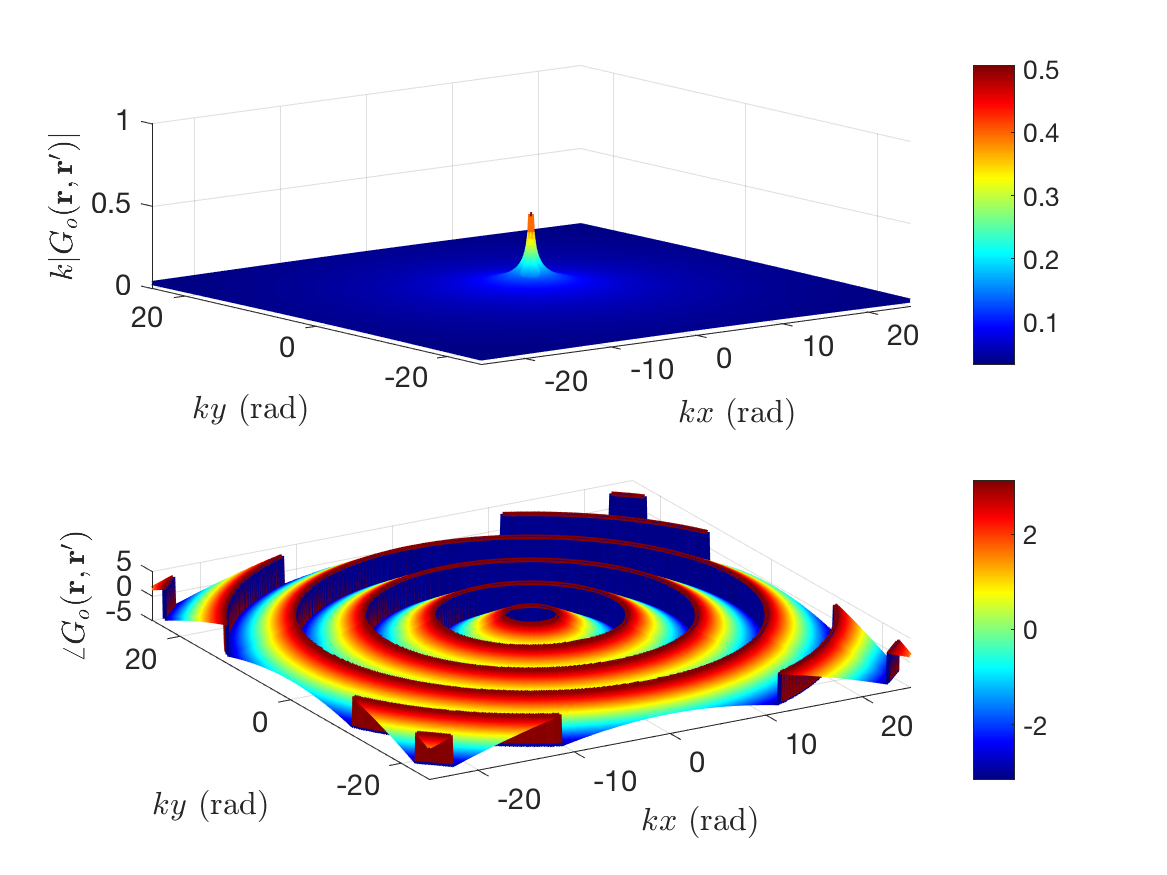
\includegraphics[width=4in]{../media/2d_fs_gf_mag.png}
\end{center}
\renewcommand{\baselinestretch}{1}
\small\normalsize
\begin{quote}
\caption[Magnitude and Phase of 2-D Free Space Green's Function]{Magnitude and Phase of 2-D Free Space Green's Function \label{gf_fig:3}}
\end{quote}
\end{figure} 
\renewcommand{\baselinestretch}{2}
\small\normalsize

\begin{figure}[ht]
\begin{center}
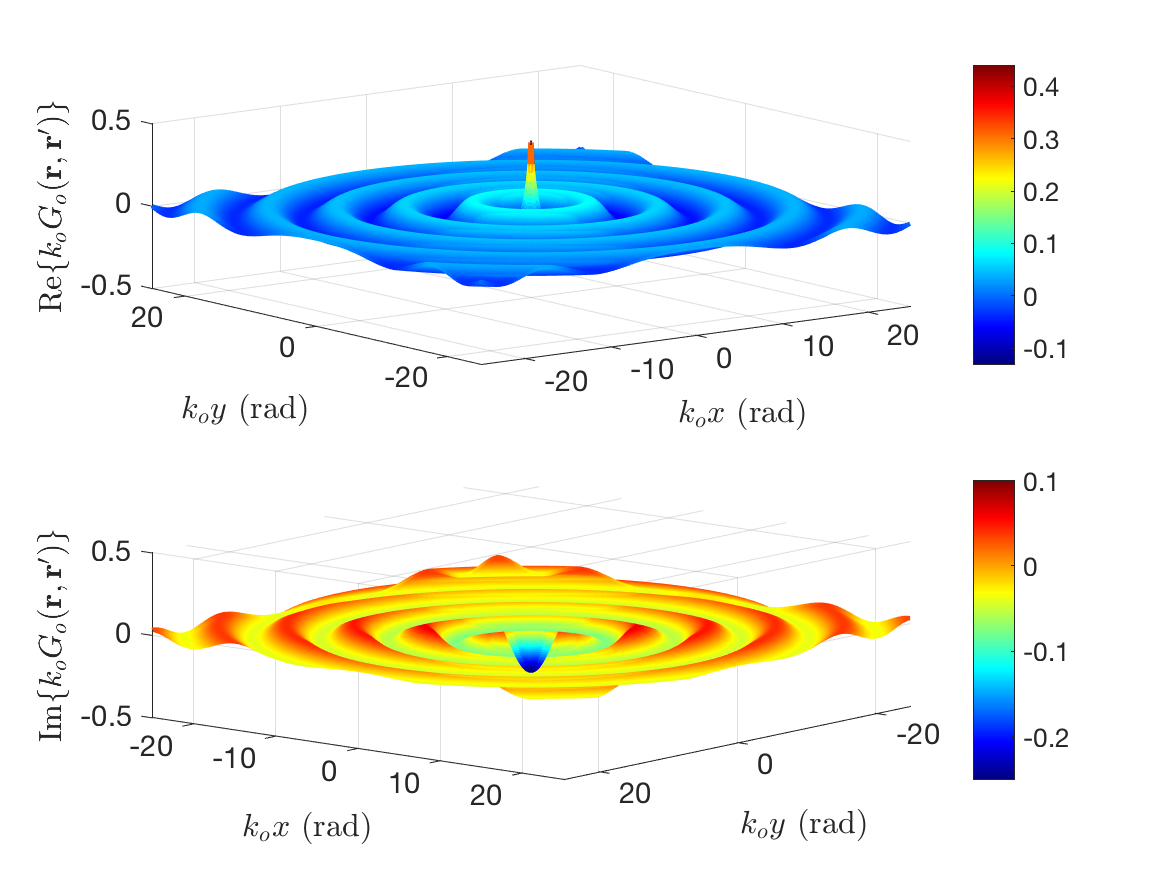
\includegraphics[width=4in]{../media/2d_fs_gf_re_im.png}
\end{center}
\renewcommand{\baselinestretch}{1}
\small\normalsize
\begin{quote}
\caption[Real and Imaginary Components of 2-D Free Space Green's Function]{Real and Imaginary Components of 2-D Free Space Green's Function \label{gf_fig:4}}
\end{quote}
\end{figure} 
\renewcommand{\baselinestretch}{2}
\small\normalsize

\subsubsection {Conversion to the Time Domain}
As in Section \ref{gf_sec:3d}, the Green's function in Equation \ref{gf_eq:40} is still in Fourier space. We can explicitly express the frequency dependence as:

\begin{equation}
G_o\left(\boldsymbol{\rho},\boldsymbol{\rho}',\omega\right) = -\frac{j}{4}H_0^{(2)}\left(\frac{\omega}{c}|\boldsymbol{\rho} - \boldsymbol{\rho}' | \right)
\label{gf_eq:40a}
\end{equation}
\renewcommand{\baselinestretch}{2} \small\normalsize

To determine the Green's function in the time domain, we need to take the inverse Fourier transform:

\begin{equation}
\begin{gathered}
G_o\left(\boldsymbol{\rho},\boldsymbol{\rho}',t\right) = \frac{1}{2\pi}\int\limits_{-\infty}^{\infty}d\omega e^{j\omega t}G_o\left(\boldsymbol{\rho},\boldsymbol{\rho}',\omega\right) \\
G_o\left(\boldsymbol{\rho},\boldsymbol{\rho}',t\right) = -\frac{j}{4}\frac{1}{2\pi}\int\limits_{-\infty}^{\infty}d\omega e^{j\omega t} H_0^{(2)}\left(\frac{\omega}{c}|\boldsymbol{\rho} - \boldsymbol{\rho}' | \right)\\
\end{gathered}
\label{gf_eq:40b}
\end{equation}
\renewcommand{\baselinestretch}{2} \small\normalsize

We can use a representation of $H_0^{(2)}$ that is related to the Mehler-Sonine integral representation \cite{nist_handbook}:

\begin{equation}
H_o^{(2)}\left(z\right) = -\frac{1}{j\pi}\int\limits_{-\infty}^{\infty}e^{-jz\cosh(\tau)}d\tau = -\frac{2}{j\pi}\int\limits_{0}^{\infty}e^{-jz\cosh(\tau)}d\tau
\label{gf_eq:40c}
\end{equation}
\renewcommand{\baselinestretch}{2} \small\normalsize

\noindent Equation \ref{gf_eq:40c} is valid for $z>0$ . Since $k_o| \boldsymbol{\rho} - \boldsymbol{\rho}'| > 0$, this condition is satisfied. Letting $\rho' \rightarrow 0$ for simplification yields:

\begin{equation}
G_o\left(\boldsymbol{\rho},0,t\right) = \frac{1}{4\pi^2}\int\limits_{-\infty}^{\infty}d\omega e^{j\omega t} \int\limits_{0}^{\infty}e^{-j\frac{\omega}{c}\rho\cosh(\tau)}d\tau\\
\label{gf_eq:40d}
\end{equation}
\renewcommand{\baselinestretch}{2} \small\normalsize

\noindent We can bring the integral over $\omega$ inside the integral over $\tau$:

\begin{equation}
\begin{gathered}
G_o\left(\boldsymbol{\rho},0,t\right) = \frac{1}{4\pi^2}\int\limits_{0}^{\infty}d\tau\int\limits_{-\infty}^{\infty}d\omega e^{j\omega t} e^{-j\frac{\omega}{c}\rho\cosh(\tau)}\\
G_o\left(\boldsymbol{\rho},0,t\right) = \frac{1}{4\pi^2}\int\limits_{0}^{\infty}d\tau\int\limits_{-\infty}^{\infty}d\omega e^{-j\omega \left(\frac{\rho \cosh(\tau)}{c} - t\right)}\\
G_o\left(\boldsymbol{\rho},0,t\right) = \frac{1}{4\pi^2}\int\limits_{0}^{\infty}d\tau\int\limits_{-\infty}^{\infty}d\omega e^{-j\omega \left(t - \frac{\rho \cosh(\tau)}{c}\right)}\\
\end{gathered}
\label{gf_eq:40e}
\end{equation}
\renewcommand{\baselinestretch}{2} \small\normalsize

\noindent Again using the definition of the delta function from Equation \ref{gf_eq:30} yields:

\begin{equation}
G_o\left(\boldsymbol{\rho},0,t\right) = \frac{1}{2\pi}\int\limits_{0}^{\infty}d\tau \delta\left(t - \frac{\rho \cosh(\tau)}{c}\right)\\
\label{gf_eq:40f}
\end{equation}
\renewcommand{\baselinestretch}{2} \small\normalsize

For $G_o\left(\boldsymbol{\rho},0,t\right)$ to be nonzero, $t - \rho \cosh(\tau)/c > 0$ for all values of $\tau$. This means $t > \rho/c$ and we can enforce this condition on $t$ through the Heaviside step function, $H\left(t -\rho/c\right)$:

 \begin{equation}
G_o\left(\boldsymbol{\rho},0,t\right) = \frac{1}{2\pi}\int\limits_{0}^{\infty}d\tau H\left(t -\frac{\rho}{c}\right) \delta\left(t - \frac{\rho \cosh(\tau)}{c}\right)
\label{gf_eq:40g}
\end{equation}
 \renewcommand{\baselinestretch}{2} \small\normalsize
 
Because the argument of the delta function is a complicated function of $t$, we need to use the composition property of the delta function \cite{arfken_weber}, \cite{gbur_math}:

 \begin{equation}
\delta\left(g(x) \right) = \sum_{\substack{a \\g(a)=0}}\frac{\delta(x-a)}{|g'(a)|}
\label{gf_eq:40h}
\end{equation}
 \renewcommand{\baselinestretch}{2} \small\normalsize
 
From Equation \ref{gf_eq:40g}, $g(\tau) = t - \rho\cosh(\tau)/c$ and the only zero  is $\tau = \cosh^{-1}\left(ct/\rho\right)$. We can now rewrite the delta function from Equation \ref{gf_eq:40g} as:

 \begin{equation}
\delta\left(t - \frac{\rho \cosh(\tau)}{c}\right) = \frac{\delta\left(\tau -\cosh^{-1}\left(\frac{ct}{\rho} \right) \right)}{\rho\sinh\left(\cosh^{-1}\left(\frac{ct}{\rho} \right) \right)}
\label{gf_eq:40i}
\end{equation}
 \renewcommand{\baselinestretch}{2} \small\normalsize
 
\noindent We can now rewrite Equation \ref{gf_eq:40g} as:

 \begin{equation}
 \begin{gathered}
G_o\left(\boldsymbol{\rho},0,t\right) = \frac{1}{2\pi}\int\limits_{0}^{\infty}d\tau H\left(t -\frac{\rho}{c}\right)  \frac{c\delta\left(\tau -\cosh^{-1}\left(\frac{ct}{\rho} \right) \right)}{\rho\sinh\left(\cosh^{-1}\left(\frac{ct}{\rho} \right) \right)}\\
G_o\left(\boldsymbol{\rho},0,t\right) = \frac{cH\left(t -\frac{\rho}{c}\right)}{2\pi \rho\sinh\left(\cosh^{-1}\left(\frac{ct}{\rho} \right) \right)}\int\limits_{0}^{\infty}d\tau \delta\left(\tau -\cosh^{-1}\left(\frac{ct}{\rho} \right) \right)\\
G_o\left(\boldsymbol{\rho},0,t\right) = \frac{cH\left(t -\frac{\rho}{c}\right)}{2\pi \rho\sinh\left(\cosh^{-1}\left(\frac{ct}{\rho} \right) \right)}
\end{gathered}
\label{gf_eq:40j}
\end{equation}
 \renewcommand{\baselinestretch}{2} \small\normalsize
 
\noindent Using the identity that $\sinh\left(\cosh^{-1}(x) \right) = \sqrt{x^2 -1}$:

 \begin{equation}
 \begin{gathered}
G_o\left(\boldsymbol{\rho},0,t\right) = \frac{cH\left(t -\frac{\rho}{c}\right)}{2\pi \rho\sqrt{\left(\frac{ct}{\rho} \right)^2 - 1}     }\\
G_o\left(\boldsymbol{\rho},0,t\right) = \frac{H\left(t -\frac{\rho}{c}\right)}{2\pi \sqrt{t^2 - \left(\frac{\rho}{c}\right)^2}     }
\end{gathered}
\label{gf_eq:40k}
\end{equation}
 \renewcommand{\baselinestretch}{2} \small\normalsize
 
\noindent Letting $t\rightarrow |t-t'|$ and $\rho \rightarrow |\boldsymbol{\rho} - \boldsymbol{\rho}'|$ yields the final result:

 \begin{equation}
\boxed{G_o\left(\boldsymbol{\rho},\boldsymbol{\rho}',t,t'\right) = \frac{H\left(|t-t'| -\frac{|\boldsymbol{\rho} - \boldsymbol{\rho}'|}{c}\right)}{2\pi \sqrt{|t-t'|^2 -\left(\frac{|\boldsymbol{\rho} - \boldsymbol{\rho}'|}{c}\right)^2 }     }}
\label{gf_eq:40l}
\end{equation}
\renewcommand{\baselinestretch}{2} \small\normalsize

\subsection {Paraxial Wave Equation} \label{gf_sec:paraxial}
In this section we derive the Green's function for the paraxial wave equation in the frequency domain.

\subsubsection {Derivation of the Paraxial Wave Equation}
We can derive the paraxial from the Helmholtz equation by assuming a wave propagating in the $x$ direction of the form $U(x,z) = A(x,z)e^{-jk_ox}$.

 \begin{equation}
 \begin{gathered}
 \left[ \nabla^2 + k_o^2\right]U = 0 \\
\left[\frac{\partial^2 }{\partial x^2} + \frac{\partial^2 }{\partial z^2} + k_o^2\right]U = 0 \\
\frac{\partial }{\partial x}\left(\frac{\partial U}{\partial x} \right) + \frac{\partial^2 U}{\partial z^2} + k_o^2 U = 0 \\
\frac{\partial }{\partial x}\left(-jk_oAe^{-jk_ox}+e^{-jk_ox}\frac{\partial A}{\partial x} \right) + e^{-jk_ox}\frac{\partial^2 A}{\partial z^2} + k_o^2 Ae^{-jk_ox} = 0 \\
-k_o^2Ae^{-jk_ox} -2jk_oe^{-jk_ox}\frac{\partial A}{\partial x}+e^{-jk_ox}\frac{\partial^2 A}{\partial x^2} + e^{-jk_ox}\frac{\partial^2 A}{\partial z^2} + k_o^2 Ae^{-jk_ox} = 0 \\
e^{-jk_ox}\left( -2jk_o\frac{\partial A}{\partial x}+\frac{\partial^2 A}{\partial x^2} + \frac{\partial^2 A}{\partial z^2}\right) = 0 \\
\end{gathered}
\label{gf_eq:41}
\end{equation}
 \renewcommand{\baselinestretch}{2} \small\normalsize
 
\noindent This gives us an equation dependent only on the amplitude, $A$

 \begin{equation}
-2jk_o\frac{\partial A}{\partial x}+\frac{\partial^2 A}{\partial x^2} + \frac{\partial^2 A}{\partial z^2} = 0 \\
\label{gf_eq:42}
\end{equation}
 \renewcommand{\baselinestretch}{2} \small\normalsize
 
 We can now apply the paraxial approximation which states that the change in the modulation function along the propagation direction is negligible over a wavelength. This can be expressed mathematically as
 
  \begin{equation}
k_o\frac{\partial A}{\partial x} >> \frac{\partial^2 A}{\partial^2 x}
\label{gf_eq:43}
\end{equation}
 \renewcommand{\baselinestretch}{2} \small\normalsize
 
 With this approximation we can neglect the 2nd derivative in $x$ and write the paraxial equation as
 
\begin{equation}
\boxed{-2jk_o\frac{\partial A}{\partial x} + \frac{\partial^2 A}{\partial z^2} = 0} \\
\label{gf_eq:44}
\end{equation}
\renewcommand{\baselinestretch}{2} \small\normalsize
 
The paraxial wave equation is a parabolic differential equation with the same structure as the diffusion equation. However, since the effective diffusion coefficient is complex, we can expect the solution to oscillate rather than decay exponentially.

Since we have reduced the original Helmholtz equation for the full propagating wave to one that is only dependent on the modulation function, we will need to scale the Green's function by $e^{-jk_ox}$ to get the full propagating wave solution.
 
\subsubsection {Green's Function Derivation in the Frequency Domain}
As stated in the previous section, the Green's function for the paraxial wave equation, $G_p$, will only define the amplitude modulation. To get the full Green's function, we will need to scale by the plane wave, $G_o= G_p e^{-jk_ox}$. We can start with substituting the Greens function into equation \ref{gf_eq:44}.

\begin{equation}
-2jk_o\frac{\partial G_p}{\partial x} + \frac{\partial^2 G_p}{\partial z^2} = -\delta(x)\delta(z)
\label{gf_eq:44a}
\end{equation}
 \renewcommand{\baselinestretch}{2} \small\normalsize
 
We can then take the Fourier transform of Equation \ref{gf_eq:44a} along $z$ and multiply both sides by $-1$.

\begin{equation}
2jk_o\frac{\partial \hat{G_p}}{\partial x} +k^2\hat{G_p} = \delta(x)
\label{gf_eq:45}
\end{equation}
 \renewcommand{\baselinestretch}{2} \small\normalsize
 
Solving away from the delta function yields the following expression for $\hat{G_p}$:

\begin{equation}
\hat{G_p}= ce^{\frac{jk^2}{2k_o}x}
\label{gf_eq:46}
\end{equation}
 \renewcommand{\baselinestretch}{2} \small\normalsize
 
To find $c$, we can integrate Equation \ref{gf_eq:45} over a small region $\pm\epsilon$ and take the limit as $x\rightarrow 0$.

\begin{equation}
\lim_{x\rightarrow 0}\int_{-\epsilon}^{\epsilon}dx\left[2jk_o\frac{\partial\hat{G_p}}{\partial x}+ k^2\hat{G_p} \right] = \lim_{x\rightarrow 0}\int_{-\epsilon}^{\epsilon}dx\delta(x)\\
\label{gf_eq:47}
\end{equation}
 \renewcommand{\baselinestretch}{2} \small\normalsize
 
\noindent $\hat{G_p}$ must be continuous, so the integral over the $k^2\hat{G_p}$ term must be 0.

\begin{equation}
\begin{gathered}
\lim_{x\rightarrow 0}2jk_o\int_{-\epsilon}^{\epsilon}dx\frac{\partial\hat{G_p}}{\partial x}= 1\\
\lim_{x\rightarrow 0}2jk_o\hat{G_p} = 1 \\
\lim_{x\rightarrow 0}2jk_oce^{\frac{jk^2}{2k_o}x} = 1\\
c = \frac{1}{j2k_o}\\
\end{gathered}
\label{gf_eq:11cb}
\end{equation}
 \renewcommand{\baselinestretch}{2} \small\normalsize
 
\noindent This yields the final expression for $\hat{G}$:

\begin{equation}
\boxed{\hat{G_p}= \frac{1}{2jk_o}e^{\frac{jk^2}{2k_o}x}}
\label{gf_eq:11cc}
\end{equation}
 \renewcommand{\baselinestretch}{2} \small\normalsize
 
\noindent To find $G_p$, we can take the inverse Fourier transform of $\hat{G_p}$:

\begin{equation}
\begin{aligned}
G_p &= \mathcal{F}^{-1}\{\hat{G_p}\} = \frac{1}{2jk_o}\frac{1}{2\pi}\int_{-\infty}^{\infty}dk e^{\frac{jk^2}{2k_o}x}e^{-jkz} \\
& = \frac{1}{2jk_o}\frac{1}{2\pi}\int_{-\infty}^{\infty}dk e^{\frac{jk^2}{2k_o}x-jkz} \\
\end{aligned}
\label{gf_eq:11d}
\end{equation}
 \renewcommand{\baselinestretch}{2} \small\normalsize
 
\noindent To solve this, we need to complete the square with respect to $k$

\begin{equation}
\begin{gathered}
\frac{jx}{2k_o}\left[k^2  -2k\frac{k_oz}{x}\right]\\
\frac{jx}{2k_o}\left[\left(k - \frac{k_oz}{x}\right)^2 - \frac{k_o^2z^2}{x^2} \right]\\
\frac{jx}{2k_o}\left(k - \frac{k_oz}{x}\right)^2 - \frac{jk_oz^2}{x}\\
\end{gathered}
\label{gf_eq:11e}
\end{equation}
 \renewcommand{\baselinestretch}{2} \small\normalsize
 
\noindent Now we can substitute into Equation \ref{gf_eq:11d}

\begin{equation}
\begin{aligned}
G_p &= \frac{1}{2jk_o}\frac{1}{2\pi}\int_{-\infty}^{\infty}dk e^{\frac{jx}{2k_o}\left(k  -\frac{k_oz}{x}\right)^2- \frac{jk_o}{2x}z^2 } \\
&= \frac{1}{2jk_o}\frac{1}{2\pi} \sqrt{\frac{\pi j2k_o}{x}}e^{-j\frac{k_o}{2x}z^2 } \\
&= \frac{1}{2jk_o}\sqrt{\frac{jk_o}{2\pi x}}\exp\left[-j\frac{k_oz^2}{2x} \right]\\
&= \sqrt{\frac{1}{8\pi j k_ox}}\exp\left[-j\frac{k_oz^2}{2x} \right]\\
\end{aligned}
\label{gf_eq:11f}
\end{equation}
 \renewcommand{\baselinestretch}{2} \small\normalsize
 
\noindent Multiplying by $e^{-jk_ox}$ yields the full Green's function.

\begin{equation}
G= \sqrt{\frac{1}{8\pi jk_ox}}\exp\left[-j\frac{k_oz^2}{2x} \right]e^{-jk_ox}
\label{gf_eq:11fa}
\end{equation}
  \renewcommand{\baselinestretch}{2} \small\normalsize
  
We can let $x\rightarrow |x-x'|$ and $x\rightarrow |z-z'|$ to represent the Green's function as traditionally shown.

\begin{equation}
\boxed{G\left(x,x',z,z' \right)= \sqrt{\frac{1}{8\pi jk_o|x-x'|}}\exp\left[-jk_o\left(|x-x'| + \frac{|z-z'|^2}{2|x-x'|}\right) \right]}\\
\label{gf_eq:11fb}
\end{equation}
 \renewcommand{\baselinestretch}{2} \small\normalsize
 
To help visualize this Green's function, the magnitude and phase is shown in Figure \ref{gf_fig:5} and the real and imaginary components are shown in Figure \ref{gf_fig:6}. Both figures show a slice of the Green's function along $z = 0$. 

\begin{figure}[ht]
\begin{center}
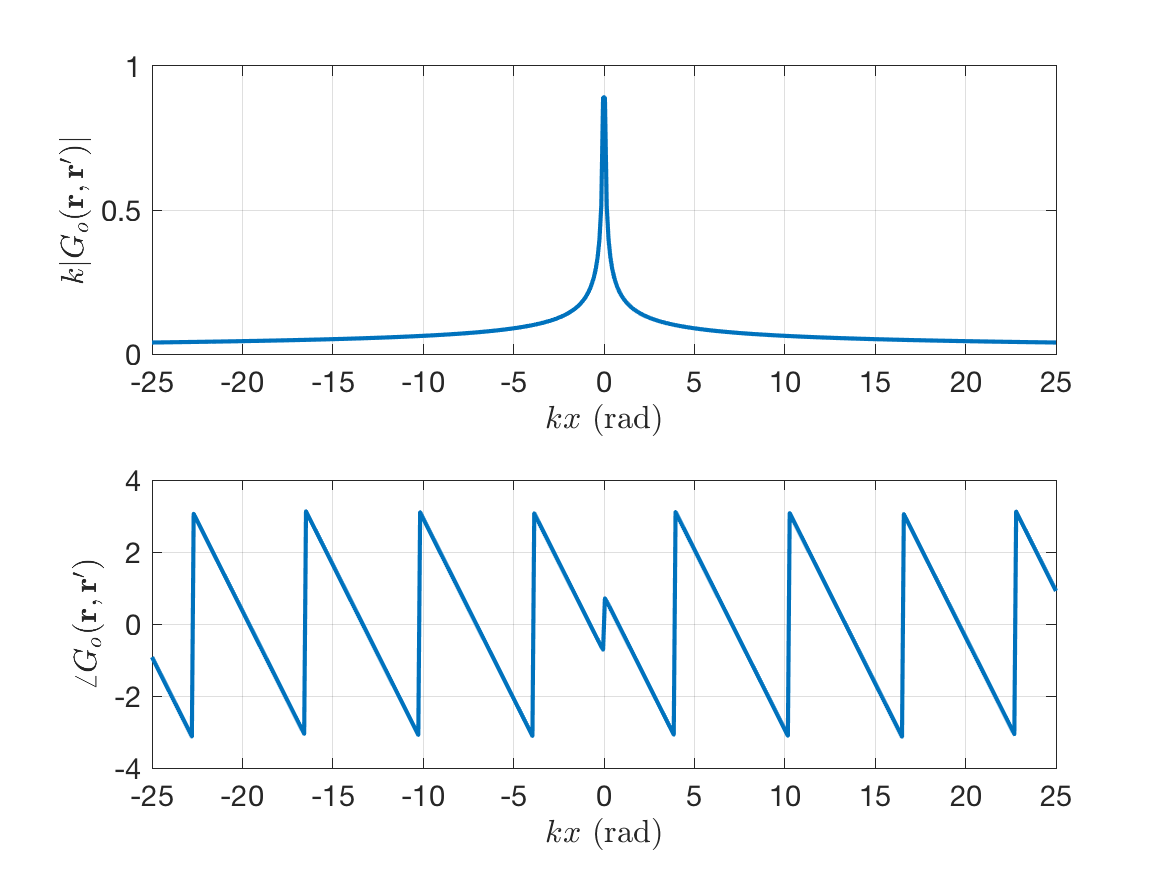
\includegraphics[width=4in]{../media/2d_paraxial_gf_mag.png}
\end{center}
\renewcommand{\baselinestretch}{1}
\small\normalsize
\begin{quote}
\caption[Magnitude and Phase of 2-D Paraxial Green's Function]{Magnitude and Phase of 2-D Paraxial Green's Function \label{gf_fig:5}}
\end{quote}
\end{figure} 
\renewcommand{\baselinestretch}{2}
\small\normalsize

\begin{figure}[ht]
\begin{center}
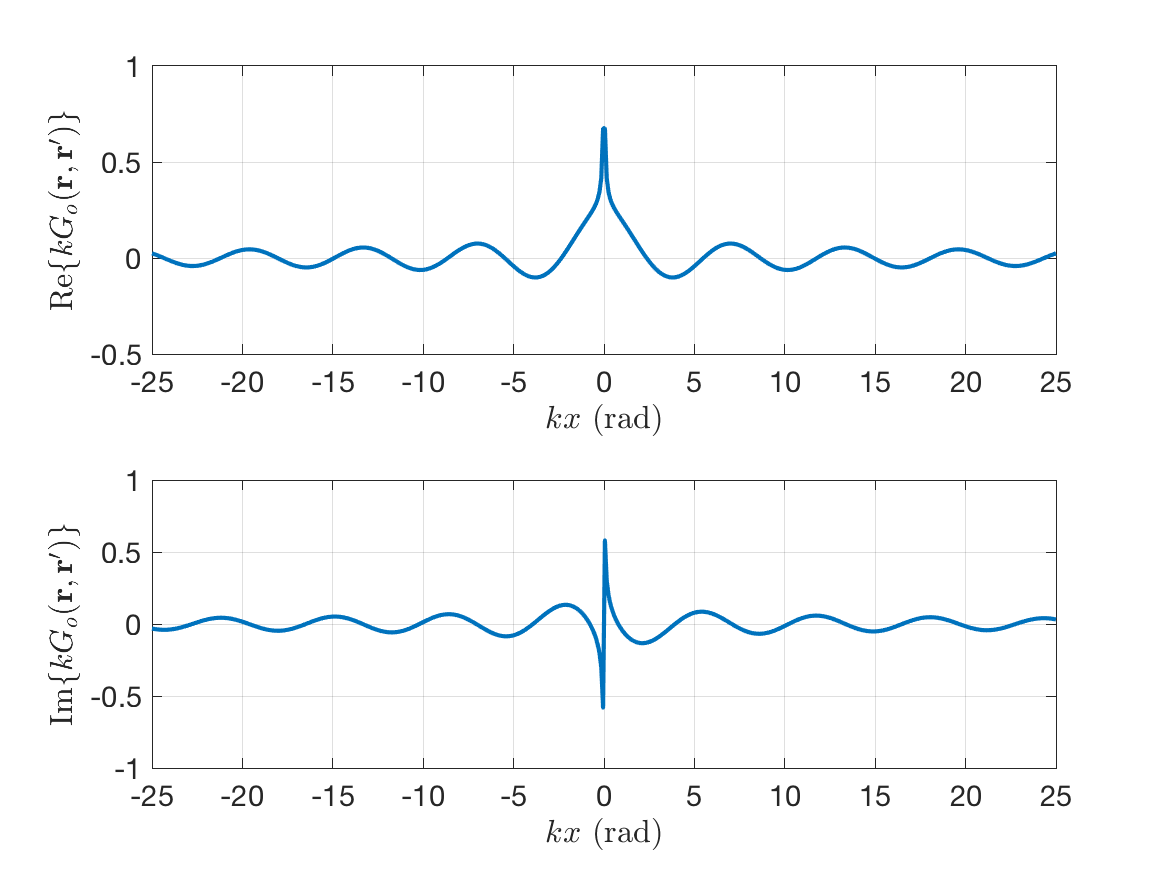
\includegraphics[width=4in]{../media/2d_paraxial_gf_re_im.png}
\end{center}
\renewcommand{\baselinestretch}{1}
\small\normalsize
\begin{quote}
\caption[Real and Imaginary Components of 2-D Paraxial Green's Function]{Real and Imaginary Components of 2-D Paraxial Green's Function \label{gf_fig:6}}
\end{quote}
\end{figure} 
\renewcommand{\baselinestretch}{2}
\small\normalsize

\subsubsection{Derivation From 3-D Free Space Green's Function}
A simpler method to derive the Green's function for the paraxial wave equation is to apply the paraxial assumption to the 3-D free space Green's function. This assumption allows us to substitute $r$ with $x$ for the amplitude, but we will need to integrate out the $y$ dependence of the phase because it is a rapidly oscillating function. We can use a binomial expansion to separate the $y$ and $z$ dependence.

\begin{equation}
r = \sqrt{x^2+y^2+z^2} \approx x + \frac{y^2}{2x}+\frac{z^2}{2x}
\label{gf_eq:11za}
\end{equation}
 \renewcommand{\baselinestretch}{2} \small\normalsize
 
\noindent The paraxial approximation of the 3-D free space Green's function is then

\begin{equation}
G_o \approx \frac{\exp\left[-jk_o\left(x+\frac{z^2}{2x} \right)\right]}{4\pi x} \exp\left[-jk_o\frac{y^2}{2x}\right]
\label{gf_eq:11zb}
\end{equation}
 \renewcommand{\baselinestretch}{2} \small\normalsize
 
\noindent We can integrate out the $y$ dependence

\begin{equation}
\int_{-\infty}^{\infty} dy \exp\left[-jk_o\frac{y^2}{2x}\right] = \sqrt{\frac{2\pi x}{jk_o}}
\label{gf_eq:11zc}
\end{equation}
 \renewcommand{\baselinestretch}{2} \small\normalsize
 
\noindent This then scales Equation \ref{gf_eq:11zb}

\begin{equation}
\begin{aligned}
G_o &= \frac{\exp\left[-jk_o\left(x+\frac{z^2}{2x} \right)\right]}{4\pi x} \sqrt{\frac{2\pi x}{jk_o}}\\
&= \sqrt{\frac{1}{j8\pi k_o x}}\exp\left[-jk_o\left(x+\frac{z^2}{2x} \right)\right]
\label{gf_eq:11zd}
\end{aligned}
\end{equation}
 \renewcommand{\baselinestretch}{2} \small\normalsize
 
\noindent Equation \ref{gf_eq:11zb} is identical to Equation \ref{gf_eq:11fa} so we get the same answer either way.

\subsection {Tabularized Green's Functions}
Table \ref{gf_tab:0} collects the various Green's functions derived in this section. Again, these were derived assuming a time dependence going as $e^{j\omega t}$.
\begin{table}[ht]
  \begin{center}
      \renewcommand{\baselinestretch}{1} \small\normalsize
  \begin{quote}
    \caption[Table of Derived Green's Functions]{Table of Derived Green's Functions\label{gf_tab:0}}
  \end{quote}
  \begin{tabular} {|c | c | c|}
    \hline
  \bf{Wave Equation} & \bf{Frequency Domain} & \bf{Time Domain}\\ \hline
  3-D Free Space & $\displaystyle\frac{e^{-jk_o|\mathbf{r} - \mathbf{r}'|}}{4\pi |\mathbf{r} - \mathbf{r}'|}$ &  $\displaystyle\frac{\delta\left(|t-t'|-\frac{|\mathbf{r}-\mathbf{r}'|}{c} \right)}{4\pi |\mathbf{r}-\mathbf{r}'|}$ \\ \hline
  2-D Free Space & $\displaystyle -\frac{j}{4}H_0^{(2)}\left(k_o|\boldsymbol{\rho} - \boldsymbol{\rho}' | \right)$ & $\displaystyle\frac{H\left(|t-t'| -\frac{|\boldsymbol{\rho} - \boldsymbol{\rho}'|}{c}\right)}{2\pi \sqrt{|t-t'|^2 -\left(\frac{|\boldsymbol{\rho} - \boldsymbol{\rho}'|}{c}\right)^2 }     }$  \\ \hline
  2-D Paraxial & $\displaystyle\sqrt{\frac{1}{8\pi jk_o|x-x'|}}\exp\left[-jk_o\left(|x-x'| + \frac{|z-z'|^2}{2|x-x'|}\right) \right]$ & N/A \\ \hline
\end{tabular}
\end{center}
\end{table}
\renewcommand{\baselinestretch}{2} \small\normalsize

\section {Propagation With Green's Functions}
This section describes how to use Green's functions to find solutions for propagation problems. We will identify the disturbance at the observation point as $U(P_2)$ and the disturbance at the source as $U(P_1)$.

\subsection {Free Space Propagation}
For free space propagation problems, there are no boundaries present and we only have the forcing function of Equation \ref{gf_eq:11} surviving so that $U(P_0) = -\int d^3r' Gf$. 

\subsubsection{Point Source}
The simplest implementation is to assume a point source, so that $f= -\alpha \delta(\mathbf{r}-\mathbf{r_o})\delta(t-t_o)$, in which case the solution simply becomes $U = G(\mathbf{r},\mathbf{r}_o,t,t_o)$. In the 3-dimensional case, the disturbance is then $U(P_0) =1/(4\pi r)\exp[-jk_or]$.

The point source approximation greatly simplifies the calculation and is adequate to capture propagation characteristics in many cases, especially at long ranges. At closer ranges, the distributed aspects of a source become apparent and may be important to include in cases such as predicting the infrared signature of objects.

\subsubsection {Diffraction through an Aperture}
The canonical diffraction problem is the propagation of light through an aperture and is heavily utilized in the field of Fourier Optics \cite{goodman_fourier} \cite{gaskill_fourier}.

\subsection{Rayleigh-Sommerfeld Diffraction Integral}
Following Huygen's principle, we can use every point in the aperture as a source for secondary waves. In order to ensure the integral over the surface vanishes at far distances, we need to apply the Sommerfeld radiation condition on the disturbance $U$

\begin{equation}
 \lim_{R\to\infty} R\left(\frac{\partial U}{\partial n} -jkU \right) = 0.
\label{gf_eq:48}
\end{equation}
\renewcommand{\baselinestretch}{2} \small\normalsize

We will assume there is no additional forcing function in the aperture so the solution from Equation \ref{gf_eq:11} is just the surface integral over the aperture.

The Rayleigh-Sommerfeld approach uses an alternative Green's function that is generated by a pair of mirrored point sources located at $\mathbf{r}_1$ and $\mathbf{r}_2$ such that $\mathbf{r}_1 = -\mathbf{r}_2$. This configuration ensures that the Green's function vanishes on the surface so the boundary conditions do not need to be applied to both $U$ and $\partial U/\partial n$. This Greens function, $G\_$, is then given as

\begin{equation}
G\_= \frac{\exp[-jk_or_1]}{4\pi r_1} - \frac{\exp[-jk_or_2]}{4\pi r_2}
\label{gf_eq:49}
\end{equation}
\renewcommand{\baselinestretch}{2} \small\normalsize

With $\theta_1$ equal to the angle between $\hat{n}$ and $\mathbf{r_1}$ and $\theta_2$ equal to the angle between $\hat{n}$ and $\mathbf{r_2}$, we can write the normal derivative, $\partial G\_/\partial n$, as 

\begin{equation}
\frac{\partial G\_}{\partial n}
=\cos(\theta_1)\left(-jk_o - \frac{1}{r_1} \right)\frac{\exp[-jk_or_1]}{4\pi r_1} -\cos(\theta_2)\left(-jk_o - \frac{1}{r_2} \right)\frac{\exp[-jk_or_1]}{4\pi r_2}
\label{gf_eq:50}
\end{equation}
\renewcommand{\baselinestretch}{2} \small\normalsize

\noindent In the aperture, $\cos(\theta_1) = -\cos(\theta_2)$ and $r_1=r_2=r$ so that

\begin{equation}
\begin{aligned}
\frac{\partial G\_}{\partial n}\bigg|_S &= -2\cos(\theta)\left(\frac{jk_o}{4\pi r} + \frac{1}{4\pi r^2}\right)\exp[-jk_or]\\
&=2\frac{\partial G}{\partial n}\bigg|_S \\
\end{aligned}
\label{gf_eq:51}
\end{equation}
\renewcommand{\baselinestretch}{2} \small\normalsize

\noindent With this Green's function in hand, we can rewrite the solution in Equation \ref{gf_eq:11} as

\begin{equation}
\begin{gathered}
U(P_2) = -\oint\limits_{S}U(S)\frac{\partial G\_}{\partial n}dS\\
= -2\oint\limits_{S}U(S)\frac{\partial G}{\partial n}dS
\end{gathered}
\label{gf_eq:52}
\end{equation}
\renewcommand{\baselinestretch}{2} \small\normalsize

This equation directly relates the disturbance at $P_2$ to the disturbance in the aperture. For the 3-dimensional case with the assumption that $1/r^2 << k_o$, we get the following expression for the Rayleigh-Sommerfeld formula, which is the mathematical representation of the Huygens-Fresnel principle.

\begin{equation}
\boxed{U(P_2) =\frac{j}{\lambda}\int_S U(S)\frac{\exp\left[-jk_o r\right]}{r}\cos(\theta)dS}
\label{gf_eq:53}
\end{equation}
\renewcommand{\baselinestretch}{2} \small\normalsize

As stated in \cite{goodman_fourier} and \cite{gaskill_fourier}, the Huygens-Fresnel principle states that the disturbance observed at a given point is the superposition of diverging spherical waves that originate at secondary points in the aperture. The diverging spherical waves are reduced in amplitude by a factor $\lambda$, scaled by a directivity pattern $\cos(\theta)$, and shifted in phase by $90^{\circ}$.

\noindent If we let $r \rightarrow |\mathbf{r}-\mathbf{r}'|$ for generality, the convolution property becomes more apparent

\begin{equation}
U(P_2) =\frac{j}{\lambda}\int_S U(S)\frac{\exp\left[-jk_o |\mathbf{r}-\mathbf{r}'|\right]}{|\mathbf{r}-\mathbf{r}'|}\cos(\theta)dS
\label{gf_eq:53a}
\end{equation}
\renewcommand{\baselinestretch}{2} \small\normalsize

Equation \ref{gf_eq:53a} tells us that propagation acts as a linear system with the convolution kernel, $h$, given as

\begin{equation}
h=\frac{j}{\lambda}\frac{\exp\left[-jk_o |\mathbf{r}-\mathbf{r}'|\right]}{|\mathbf{r}-\mathbf{r}'|}\cos(\theta)
\label{gf_eq:53b}
\end{equation}
\renewcommand{\baselinestretch}{2} \small\normalsize

\subsubsection{Fresnel Diffraction}
The Fresnel approximation is essentially the paraxial approximation but retaining all 3 dimensions. If we take a binomial expansion of $r$ but keep both the $x$ and $y$ components and assume the source plane is located at $z=0$, we can approximate $r$ as

\begin{equation}
r\approx z + \frac{(x-x’)^2}{2z}+\frac{(y-y’)^2}{2z}
\label{gf_eq:53c}
\end{equation}
\renewcommand{\baselinestretch}{2} \small\normalsize

Here, $x'$ and $y'$ represent the coordinates in the source plane and $x$ and $y$ represent the coordinates in the observation plane. Because of the quadratic nature, the phase will rapidly oscillate as we move off axis. This means only a narrow region around the axis will contribute significantly and we can use the principle of stationary phase \cite{gbur_math} to extend the integration limits to $\pm \infty$. With the substitution $\cos(\theta) = z/r \approx 1$, we can now rewrite Equation \ref{gf_eq:53} as

\begin{equation}
\boxed{U(P_2) =\frac{je^{-jk_oz}}{\lambda z}\int_{-\infty}^{\infty} U(x’,y’)\exp\left[-j \frac{k}{2z}\left([x-x’]^2 + [y-y’]^2 \right) \right]dx’ dy’}
\label{gf_eq:53d}
\end{equation}
\renewcommand{\baselinestretch}{2} \small\normalsize

Equation \ref{gf_eq:53d} is the Fresnel approximation of the diffraction integral and represents propagation as convolution with a kernel containing a quadratic phase factor

\begin{equation}
h = \frac{je^{-jk_o z}}{\lambda z}\exp\left[-j\frac{k_o}{2z}\left(x^2 + y^2 \right) \right]
\label{gf_eq:53e}
\end{equation}
\renewcommand{\baselinestretch}{2} \small\normalsize

From \cite{goodman_fourier}, the Fresnel approximation is usually sufficient when $z\geq D_{\text{max}}^2/16$, where $D_{\text{max}}$ is the maximum spatial extent, $D_{\text{max}} = x_{\text{max}}^2 + y_{\text{max}}^2$. 

\subsubsection{Fraunhofer Diffraction}
If we allow the wave to propagate further, the quadratic phase factor will not contribute significantly and we can factor it out of the integral. This approximation is valid when the propagation distance meets the following criteria.

\begin{equation}
z >> \frac{k_oD_{\text{max}}}{2}
\label{gf_eq:53f}
\end{equation}
\renewcommand{\baselinestretch}{2} \small\normalsize

For clarity, we typically replace $x'$ with $\xi$ and $y'$ with $\eta$ so that Equation \ref{gf_eq:53d} becomes

\begin{equation}
U(P_2) =\frac{je^{-jk_oz}}{\lambda z}\int_{-\infty}^{\infty} U(\xi,\eta)\exp\left[-j \frac{k}{2z}\left([x-\xi]^2 + [y-\eta]^2 \right) \right]d\xi d\eta
\label{gf_eq:53g}
\end{equation}
\renewcommand{\baselinestretch}{2} \small\normalsize

We can neglect the $\xi^2$ and $\eta^2$ terms in the exponential and let $(x-\xi)^2 \approx x^2-2x\xi$ and $(y-\eta)^2\approx y^2-2y\eta$. We can factor out the quadratic phase in terms of observation coordinates, $x$ and $y$, and rewrite Equation \ref{gf_eq:53g} as

\begin{equation}
\boxed{U(P_2) =\frac{je^{-jk_oz}e^{-j\frac{k_o}{2z}(x^2+y^2)}}{\lambda z}\int_{-\infty}^{\infty} U(\xi,\eta)\exp\left[j2\pi\left(\frac{x}{\lambda z}\xi + \frac{y}{\lambda z}\eta \right) \right]d\xi d\eta}
\label{gf_eq:53h}
\end{equation}
\renewcommand{\baselinestretch}{2} \small\normalsize

Equation \ref{gf_eq:53h} is the Fraunhofer approximation and is simply the spatial Fourier transform of the aperture with spatial frequencies $f_x = x/(\lambda z)$ and $f_y = y/(\lambda z)$ \cite{goodman_fourier} \cite{gaskill_fourier}. In other words, the spatial frequencies are the source coordinates at the observation plane divided by the product of the wavelength with the propagation distance.

\subsection {Diffraction from a Planar Surface}
We can treat diffraction from a planar surface in the same fashion as diffraction through an aperture but we will need to include a reflection coefficient, $\Gamma$. As a particular example, the surface of the ocean can be approximated as a planar surface when the ocean wave heights are much smaller than the altitude of interest.

\subsubsection{Integral Solution for Reflected Ray}
In this section, we will derive the propagation integral for a wave that is reflected off an ocean surface with small random components using a paraxial Green's function. The geometry is shown in Figure \ref{gf_fig:15}, where $\tilde{x}$, is the region over which the energy is significantly reflected, $x_m$ is the primary point of reflection, $L_1$ is the direct path, $L_2$ and $L_3$ are the path lengths for the various reflected rays, $s(x)$ is the altitude of the sea surface at $x$, $h_2$ is the altitude of the receiver at $P_2$, $h_1$ is the altitude of the transmitter at $P_1$, and $L$ is the ground distance between $P_1$ and $P_2$. 

\begin{figure}[ht]
  \begin{center}
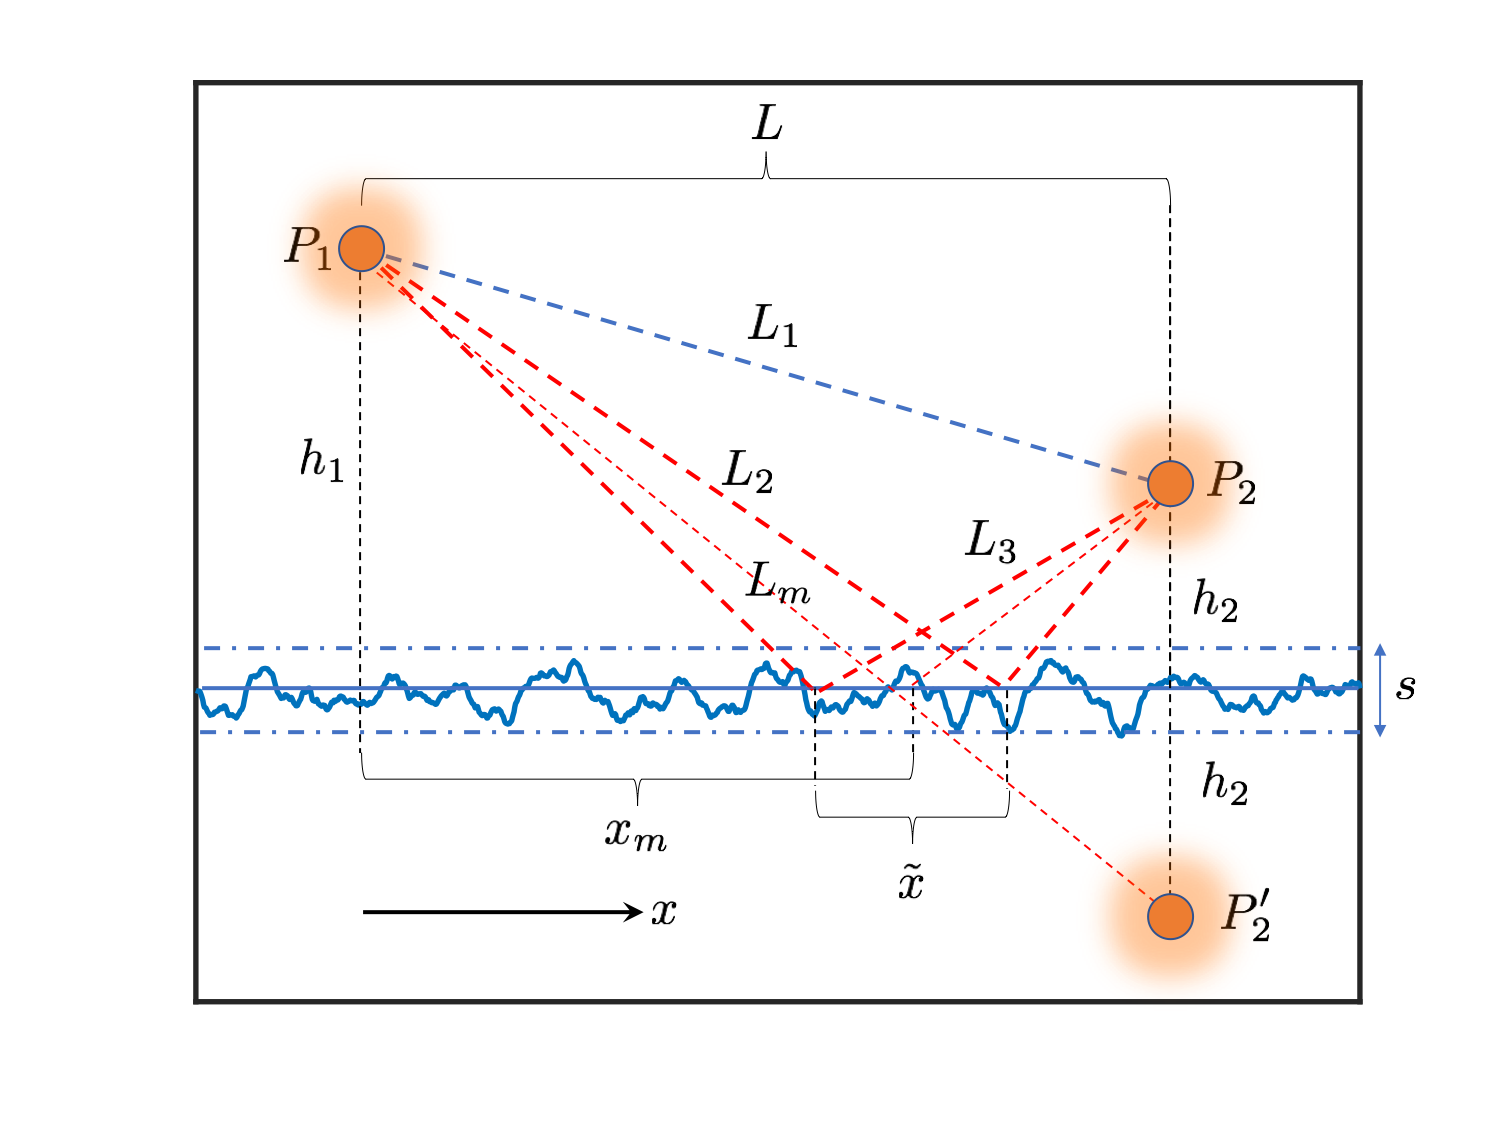
\includegraphics[width=5in]{../media/analysis/multipath_layout.png}
  \end{center}
  \renewcommand{\baselinestretch}{1} \small\normalsize
  \begin{quote}
    \caption[Geometry for Diffraction Along the Sea Surface]{Geometry for Diffraction Along the Sea Surface\label{gf_fig:15}}
  \end{quote}
\end{figure}
\renewcommand{\baselinestretch}{2} \small\normalsize

We can use Equation \ref{gf_eq:52} with the paraxial Green's function. The surface normal is now given as $\hat{z}$, so we only need to take the derivative with respect to $z$. The reflected wave along $L_3$ will then be given by

\begin{equation}
\begin{aligned}
U(P_2) &= 2jk_o\int\limits_{0}^{L}dx\Gamma U(s)\frac{z}{x}\sqrt{\frac{1}{8\pi jk_o x}}\exp\left[-jk_o\left(x +\frac{z^2}{2x} \right) \right] \\
&= \int\limits_{0}^{L}dx\Gamma U(s)\frac{z}{x}\sqrt{\frac{jk_o}{2\pi x}}\exp\left[-jk_o\left(x +\frac{z^2}{2x} \right) \right] \\
\end{aligned}
\label{gf_eq:55}
\end{equation}
\renewcommand{\baselinestretch}{2} \small\normalsize

From the geometry in Figure \ref{gf_fig:15}, we are shifting the starting point for the return path by $x$ and we need to let $x \rightarrow L-x$ and $z \rightarrow h_2-s$ so that we now have

\begin{equation}
\begin{aligned}
U_2(P_2) &= \int\limits_{0}^{L}dx\Gamma U(s)\frac{h_2-s}{L-x}\sqrt{\frac{jk_o}{2\pi (L-x)}}\exp\left[-jk_o\left(L-x +\frac{(h_2-s)^2}{2(L-x)} \right) \right] \\
&= \int\limits_{0}^{L}dx\Gamma U(s)\frac{h_2-s}{L-x}\sqrt{\frac{jk_o}{2\pi (L-x)}}\exp\left[-jk_oL_3\right] \\
\end{aligned}
\label{gf_eq:56}
\end{equation}
\renewcommand{\baselinestretch}{2} \small\normalsize

The reflected wave solution at the sea surface, $U_2(s)$, follows from the free space solution, where $z \rightarrow h_1-s$.

\begin{equation}
\begin{aligned}
U_2(s) &= \sqrt{\frac{1}{8\pi jk_ox}}\exp\left[-jk_oL_2\right]\\
\end{aligned}
\label{gf_eq:57}
\end{equation}
\renewcommand{\baselinestretch}{2} \small\normalsize

\noindent The full solution for the reflected wave is then 
\begin{equation}
\begin{aligned}
U_2(P_2) &= \int_0^L dx \Gamma \sqrt{\frac{1}{8\pi j k_o x}}\exp[-jk_oL_2]\frac{h_2-s}{L-x}\sqrt{\frac{jk_o}{2\pi(L-x)}}\exp[-jk_oL_3]\\
&= \frac{1}{4\pi}\int_0^L dx \Gamma \sqrt{\frac{1}{x}}\sqrt{\frac{1}{L-x}}\frac{h_2-s}{L-x}\exp\left[-jk_o\left(L_2+L_3\right) \right]
\label{gf_eq:58}
\end{aligned}
\end{equation}
\renewcommand{\baselinestretch}{2} \small\normalsize

\subsubsection{Asymptotic Approximation for Deterministic Component}
We can simplify the various path lengths in Figure \ref{gf_fig:15} through a binomial expansion. Here $L_{so}$ represents the shortest orbit path, which would be given as a straight line between $P_1$ and the mirror image of $P_2$. 

\begin{equation}
\begin{aligned}
L_1 & = \sqrt{L^2 + (h_1-h_2)^2}  \approx L + \frac{(h_1 - h_2)^2}{2L}\\
L_{so} & = \sqrt{L^2 + (h_1+h_2)^2}  \approx L + \frac{(h_1 + h_2)^2}{2L}\\
L_2 &= \sqrt{x^2 + \left( h_1 - s(x)\right)^2}  \approx x + \frac{(h_1-s(x))^2}{2x}\\
L_3 & = \sqrt{\left(L - x\right)^2 + \left( h_2 - s(x)\right)^2}  \approx L-x + \frac{(h_2 - s(x))^2}{2\left(L-x\right)}\\
\end{aligned}
\label{gf_eq:59}
\end{equation}
\renewcommand{\baselinestretch}{2} \small\normalsize

The path length for a given reflected ray, $L_r$ is given by
\begin{equation}
\begin{aligned}
L_r &= L_2 + L_3 \\
& = x + \frac{h_1^2-2h_1s(x)}{2x} +  L-x + \frac{h_2^2 - 2h_2s(x)}{2\left(L-x\right)} \\
& = L + \frac{1}{2}\left[\frac{h_1^2}{x} + \frac{h_2^2}{L-x} \right] - s(x)\left[ \frac{h_1}{x} + \frac{h_2}{L-x}\right] \\
&= L + L_0 - L_s
\end{aligned}
\label{gf_eq:60}
\end{equation}
\renewcommand{\baselinestretch}{2} \small\normalsize

Here $L_0$ represents the deterministic component due to reflection from the surface and $L_s$ represents the random component due to reflection from the surface. The reflection point from the 2-ray model, $x_m$, should be a saddle point and provide the dominant contribution. We can therefore perform a Taylor expansion of $L_0$ about $x_m$.

\begin{equation}
L_0 \approx L_0(x_m) + \frac{1}{2}\frac{d^2L_0}{dx^2}\bigg|_{x_m}(x-x_m)^2
\label{gf_eq:61}
\end{equation}
\renewcommand{\baselinestretch}{2} \small\normalsize

\begin{equation}
\frac{dL_0}{dx} = \frac{1}{2}\left[\frac{-h_1^2}{x^2} + \frac{h_2^2}{(L-x)^2} \right]
\label{gf_eq:62}
\end{equation}
\renewcommand{\baselinestretch}{2} \small\normalsize

\begin{equation}
\frac{d^2L_0}{dx^2} = \frac{h_1^2}{x^3} + \frac{h_2^2}{(L-x)^3} 
\label{gf_eq:63}
\end{equation}
\renewcommand{\baselinestretch}{2} \small\normalsize
\noindent Since $\frac{dL_0}{dx}\big|_{x_m} = 0$, we can solve for $x_m$

\begin{equation}
\begin{gathered}
\frac{-h_1^2}{x_m^2} + \frac{h_2^2}{(L-x_m)^2} = 0\\
\frac{-h_1}{x_m} + \frac{h_2}{L-x_m} = 0\\
\frac{h_1}{x_m} = \frac{h_2}{L-x_m}\\
h_1(L-x_m) = h_2x_m\\
x_m = \frac{h_1L}{h_1+h_2}
\end{gathered}
\label{gf_eq:64}
\end{equation}
\renewcommand{\baselinestretch}{2} \small\normalsize

\noindent This gives the following for the lowest Taylor series terms:

\begin{equation}
\begin{aligned}
L_0(x_m) &= \frac{(h_1+h_2)^2}{2L} \\
L_0''=\frac{d^2L_0}{dx^2}\bigg|_{x_m}  &= \frac{(h_1+h_2)^4}{h_1h_2L^3} \\
L_s(x_m) &= \frac{2s(x)(h_1 + h_2)}{L}\\
\end{aligned}
\label{gf_eq:65}
\end{equation}
\renewcommand{\baselinestretch}{2} \small\normalsize

\noindent The expansion of $L_0$ is then

\begin{equation}
L_0 \approx \frac{(h_1+h_2)^2}{2L} + \frac{(h_1+h_2)^4}{2h_1h_2L^3}(x-x_m)^2
\label{gf_eq:66}
\end{equation}
\renewcommand{\baselinestretch}{2} \small\normalsize

\noindent We can now substitute into the exponential term of Equation \ref{gf_eq:58}
\begin{equation}
\begin{aligned}
&\exp\left[-jk_o\left( L_2 + L_3\right) \right] \\
&= \exp\left[-jk_o\left( L+L_0-L_s\right) \right]\\
&= \exp\left[-jk_o\left( L+L_0(x_m) + \frac{L_0''}{2}(x-x_m)^2-L_s\right) \right]\\
&= \exp\left[-jk_o\left( L+\frac{(h_1+h_2)^2}{2L} + \frac{L_0''}{2}(x-x_m)^2-L_s\right)\right]\\
&=\exp\left[-jk_o\left(L_{so}+\frac{L_0''}{2}(x-x_m)^2-L_s\right)\right]\\
&=\exp\left[-jk_oL_{so}\right]\exp\left[-jk_o\left(\frac{L_0''}{2}(x-x_m)^2-\frac{2s(h_1+h_2)}{L}\right)\right]\\
&=\exp\left[-jk_oL_{so}\right]\exp\left[\frac{-jk_oL_0''}{2}(x-x_m)^2+\frac{j2k_os(h_1+h_2)}{L}\right]\\
\label{gf_eq:67}
\end{aligned}
\end{equation}
\renewcommand{\baselinestretch}{2} \small\normalsize

Because $L_{so}$ is not dependent on $x$, it can come outside of the integral.

\subsubsection{Asymptotic Approximation for Random Component}
 If we assume that $L_s$ is locally sinusoidal with amplitude $\sigma$, frequency $k_{\omega}$, and phase $\theta$, we can approximate the exponential term as 
\begin{equation}
\begin{aligned}
\exp\left[jk_oL_s\right] =\exp\left[j\sigma \sin\left(k_{\omega} \tilde{x} + \theta\right) \right]
\end{aligned}
\label{gf_eq:68}
\end{equation}
\renewcommand{\baselinestretch}{2} \small\normalsize

\noindent From Equation \ref{gf_eq:67}, the random amplitude, $\sigma$, is given by
\begin{equation}
\begin{aligned}
\sigma = k_oL_s = \frac{2k_os(h_1+h_2)}{L}
\end{aligned}
\label{gf_eq:69}
\end{equation}
\renewcommand{\baselinestretch}{2} \small\normalsize

We can then use the Jacobi-Anger expansion \cite{gbur_math} to convert the exponential term on the far right hand side into an infinite sum of Bessel functions.
\begin{equation}
\begin{aligned}
K_r(\tilde{x}) &=\exp\left[j\sigma \sin\left(k_{\omega} \tilde{x} + \theta\right) \right] \\ &=\sum_{l=-\infty}^{\infty}J_l(\sigma)\exp\left[jl(k_{\omega}\tilde{x} + \theta) \right] \\
&=\sum_{l=-\infty}^{\infty}J_l(\sigma)\exp\left[jl\theta\right]\exp\left[jlk_{\omega}\tilde{x}\right] 
\end{aligned}
\label{gf_eq:70}
\end{equation}
\renewcommand{\baselinestretch}{2} \small\normalsize

The Bessel functions only depend on $\sigma$ and not $\tilde{x}$, so they will come outside of the integral as well.

\subsection {Knife Edges and Non-planar Terrain}
Following \cite{whitteker_diffraction}, we can formulate the integral in a direction perpendicular to the surface and treat subsequent obstacles as knife edges.

\subsection {Optical Propagation Through Turbulence}

\subsection{Polarization}
In the scalar theory presented here, there is no sense of polarization. This means that once set, the polarization will be constant for all time. Polarization is accounted for through the reflection coefficients and boundary conditions as those implicitly have polarization dependence.


\newpage
\appendix
\renewcommand{\thechapter}{B}
\renewcommand{\chaptername}{Appendix}
\chapter{Saddle Point Method}\label{appendix_saddle_point_method}
A contour integral representation of the Bessel function in the complex $z$-plane is \cite{arfken_weber}, \cite{nist_handbook}:

\begin{equation}
  J_{\nu}(x) = \frac{1}{j2\pi}\int\limits_{\mathcal{C}}e^{\frac{1}{2}x\left(z- \frac{1}{z} \right)} \frac{dz}{z^{\nu+1}}
  \label{sp_eq:1}
\end{equation}
\renewcommand{\baselinestretch}{2} \small\normalsize

The integrand is multi-valued when $\nu$ is not an integer, so we can define a branch cut along the real axis and the overall contour, $\mathcal{C}$, as shown in Figure \ref{sp_fig:1}.

\begin{figure}[H]
  \begin{center}
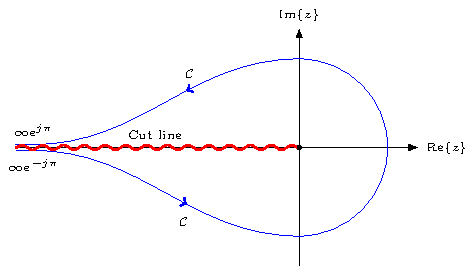
\includegraphics[width=5in]{../media/hankel_contours-figure0.pdf}
  \end{center}
  \renewcommand{\baselinestretch}{1} \small\normalsize
  \begin{quote}
    \caption[Complex Contour for Bessel Function]{ Complex Contour for Bessel Function\label{sp_fig:1}}
  \end{quote}
\end{figure}
\renewcommand{\baselinestretch}{2} \small\normalsize

We can deform the contour, $\mathcal{C}$, so that it goes to the origin and then split it into two parts, an upper contour ($\mathcal{C}_1$) and a lower contour ($\mathcal{C}_2$). Integration along the upper contour represents the Hankel function of the first kind, while integration along the lower contour represents the Hankel function of the first kind. The resulting contour is shown in Figure \ref{sp_fig:2}.

\begin{figure}[H]
  \begin{center}
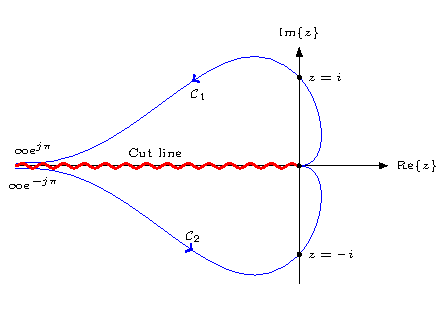
\includegraphics[width=5in]{../media/hankel_contours-figure1.pdf}
\end{center}
  \renewcommand{\baselinestretch}{1}\small\normalsize
  \begin{quote}
    \caption[Complex Contour for Hankel Functions]{Complex Contour for Hankel Functions\label{sp_fig:2}}
  \end{quote}
\end{figure}
\renewcommand{\baselinestretch}{2} \small\normalsize

The integral representations of the Hankel functions are then:
\begin{equation}
  \begin{gathered}
    H_{\nu}^{(1)}(x) = \frac{1}{j\pi}\int\limits_{\mathcal{C}_1}e^{\frac{1}{2}x\left(z- \frac{1}{z} \right)} \frac{dz}{z^{\nu+1}} \\
    H_{\nu}^{(2)}(x) = \frac{1}{j\pi}\int\limits_{\mathcal{C}_2}e^{\frac{1}{2}x\left(z- \frac{1}{z} \right)} \frac{dz}{z^{\nu+1}} 
    \end{gathered}
  \label{sp_eq:2}
  \end{equation}
\renewcommand{\baselinestretch}{2} \small\normalsize

We can find an asymptotic solution of the Hankel functions through the saddle point method, which applies to integrals in the form of $I = \int\limits_{\mathcal{C}}g(z)e^{xh(z)}dz$. We will work with the Hankel function of the second kind, $H_{\nu}^{(2)}$, as that represents a forward traveling wave.

The general idea of the saddle point method is expand the exponential term, $h(z)$ in a Taylor series about the saddle point so that the first derivative of $h$ goes to zero. We will use the phase of $h$ to ensure the dominant contribution to the integral comes from the saddle point. In Equation \ref{sp_eq:2}, $h = \frac{1}{2}\left(z-\frac{1}{z}\right)$, so the first derivative is $\frac{dh}{dz} = \frac{1}{2}\left(1+\frac{1}{z^2}\right)$, and the second derivative is $\frac{d^2h}{dz^2} = -\frac{1}{z^3}$. From the first derivative, $h$ has a saddle point ($\frac{dh}{dz}=0$) at $z=\pm j$. Along contour $\mathcal{C}_2$, the only saddle point is $z=-j$, so that is the one we will use.

The Taylor expansion of $h$ is then:

\begin{equation}
  \begin{gathered}
    h(z) \approx h\bigg|_{z=-j} + \frac{1}{2}\frac{d^2h}{dz^2}\bigg|_{z=-j}\left(z+j \right)^2\\
    h(z) \approx -j + \frac{j}{2}\left(z+j \right)^2 
    \end{gathered}
  \label{sp_eq:3}
  \end{equation}
\renewcommand{\baselinestretch}{2} \small\normalsize

Substituting this approximation for $h$ into Equation \ref{sp_eq:2} and remembering that $g(z) \rightarrow g(z)|_{z=-j}$ yields:

\begin{equation}
  \begin{gathered}
    H_{\nu}^{(2)}(x) \approx \frac{1}{j\pi}\int\limits_{\mathcal{C}_2}e^{x\left[-j + \frac{j}{2}\left(z+j \right)^2 \right]} \frac{dz}{(-j)^{\nu+1}} \\
    H_{\nu}^{(2)}(x) \approx \frac{1}{j\pi}e^{-jx}\int\limits_{\mathcal{C}_2}e^{x\frac{j}{2}\left(z+j \right)^2}(-j)^{-\nu - 1} dz \\
    H_{\nu}^{(2)}(x) \approx \frac{1}{\pi}e^{-jx}e^{-j\frac{\pi}{2}}e^{-j\frac{3\pi}{2}\left(\nu +1\right)}\int\limits_{\mathcal{C}_2}e^{x\frac{j}{2}\left(z+j \right)^2} dz \\
    H_{\nu}^{(2)}(x) \approx \frac{1}{\pi}e^{-j\left[x +\frac{\pi}{2} +\frac{3\pi}{2} + \nu\frac{3\pi}{2}\right]}\int\limits_{\mathcal{C}_2}e^{x\frac{j}{2}\left(z+j \right)^2} dz \\
     H_{\nu}^{(2)}(x) \approx \frac{1}{\pi}e^{-j\left[x - \nu\frac{\pi}{2}\right]}\int\limits_{\mathcal{C}_2}e^{x\frac{j}{2}\left(z+j \right)^2} dz 
    \end{gathered}
  \label{sp_eq:4}
  \end{equation}
\renewcommand{\baselinestretch}{2} \small\normalsize

We need to ensure that we approach the saddle point along the path of steepest descent, where the path $\mathcal{C}_2$ travels from $\infty$ to $0$ with $z$ having negative phase. By inspection we can see that the condition $\left(z+j \right)^2 \rightarrow j$ forces the integral to go to zero for large $x$. We can write this condition more explicitly in terms of phase as:

\begin{equation}
  \begin{gathered}
    \left(z + j \right)^2=j \\
    r^2e^{j2\theta} = e^{j\frac{\pi}{2}} \\
    \theta = \frac{\pi}{4}
    \end{gathered}
  \label{sp_eq:5}
  \end{equation}
\renewcommand{\baselinestretch}{2} \small\normalsize

Equation \ref{sp_eq:5} tells us that the path of integration must enter the saddle point ($z=-j$) with a phase angle of $\frac{\pi}{4}$ radians. We can use a substitution of variables, $t=(z+j)e^{j\frac{\pi}{4}}$, so that $dt = dze^{j\frac{\pi}{4}}$:

\begin{equation}
  \begin{gathered}
    H_{\nu}^{(2)}(x) \approx \frac{1}{\pi}e^{-j\left[x - \nu\frac{\pi}{2}\right]}\int\limits_{\mathcal{C}_2}e^{x\frac{j}{2}t^2e^{j\frac{\pi}{2}}} dte^{j\frac{\pi}{4}} \\
    H_{\nu}^{(2)}(x) \approx \frac{1}{\pi}e^{-j\left[x - \nu\frac{\pi}{2}\right]}e^{j\frac{\pi}{4}}\int\limits_{\mathcal{C}_2}e^{-\frac{xt^2}{2}} dt \\
     H_{\nu}^{(2)}(x) \approx  \frac{1}{\pi}e^{-j\left[x - \nu\frac{\pi}{2} - \frac{\pi}{4}\right]}\int\limits_{-\infty}^{\infty}e^{-\frac{xt^2}{2}} dt \\
    H_{\nu}^{(2)}(x) \approx \frac{1}{\pi}e^{-j\left[x - \nu\frac{\pi}{2} - \frac{\pi}{4}\right]}\sqrt{\frac{2\pi}{x}}\\
    \end{gathered}
  \label{sp_eq:6}
  \end{equation}
\renewcommand{\baselinestretch}{2} \small\normalsize

\noindent A final simplification yields the asymptotic form of the Hankel function:
\begin{equation}
    \boxed{H_{\nu}^{(2)}(x) \approx \sqrt{\frac{2}{\pi x}}e^{-j\left[x - \nu\frac{\pi}{2} - \frac{\pi}{4}\right]}}
  \label{sp_eq:7}
  \end{equation}
\renewcommand{\baselinestretch}{2} \small\normalsize

Figure \ref{sp_fig:3} shows a comparison between the real and imaginary components of the analytic and asymptotic forms of the Hankel function, $H_0^{(2)}$, and demonstrates that the asymptotic form is valid for large $x$.

\begin{figure}[H]
  \begin{center}
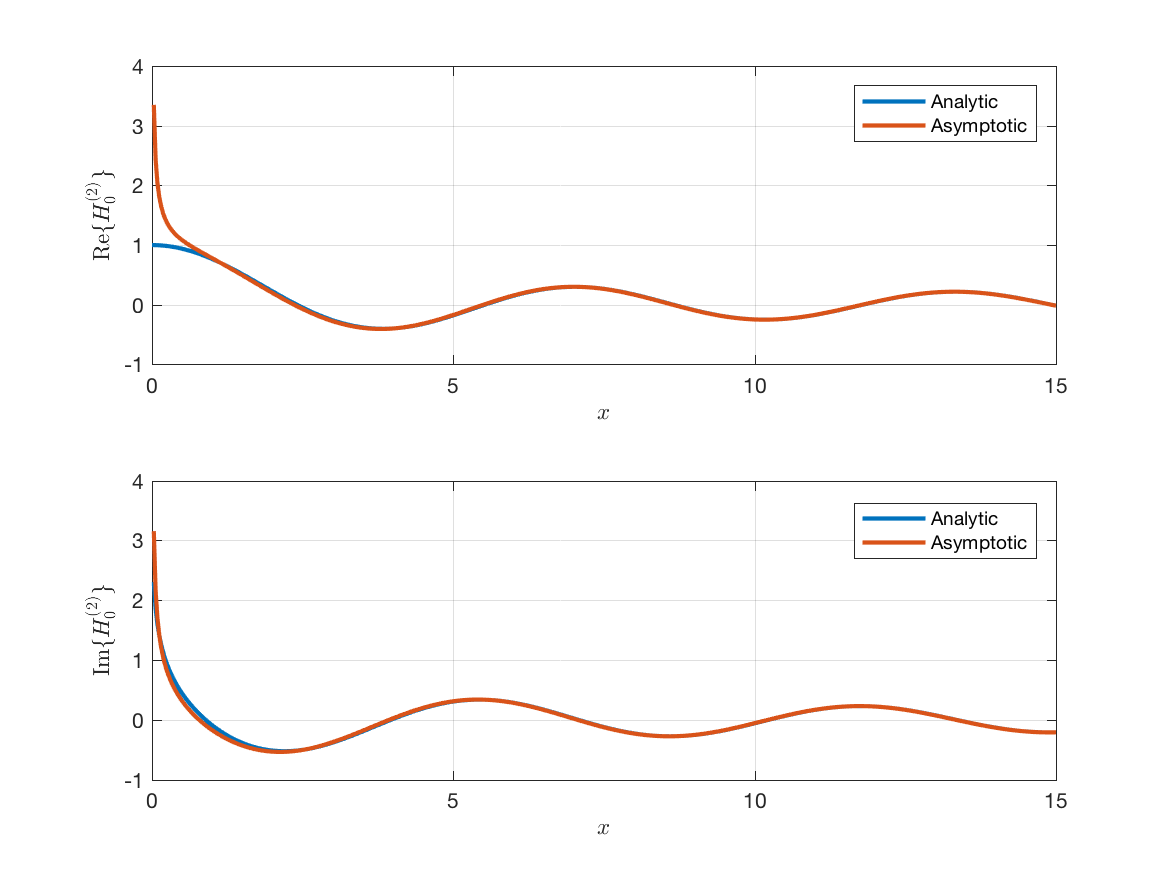
\includegraphics[width=5in]{../media/hankel_error.png}
\end{center}
  \renewcommand{\baselinestretch}{1}\small\normalsize
  \begin{quote}
    \caption[Analytic vs. Asymptotic Forms of Hankel Function]{Analytic vs. Asymptotic Forms of Hankel Function\label{sp_fig:3}}
  \end{quote}
\end{figure}
\renewcommand{\baselinestretch}{2} \small\normalsize



\renewcommand{\baselinestretch}{1}
\small\normalsize
\newpage

\newpage
\bibliographystyle{unsrt} 
\bibliography{background_bib}


\end{document}












